\documentclass{iutbscthesis}

% ---------------------------------------------------------------- extra packages
\usepackage{tikz}
\usetikzlibrary{arrows.meta, positioning, fit, calc, shapes.geometric, backgrounds}
\usepackage{algorithm}
\usepackage{algpseudocode}
\usepackage{multirow}
\usepackage{makecell}
\usepackage{longtable}
\usepackage{tabularx}
\usepackage{xcolor}
\usepackage[skins,breakable]{tcolorbox}
\usepackage{enumitem}
\setlist{itemsep=2pt, topsep=4pt}

\definecolor{cfix}{HTML}{36649E}
\definecolor{cvt}{HTML}{CE7B1A}
\definecolor{catk}{HTML}{B22D2D}
\definecolor{boxbg}{HTML}{F4F6FA}

\newtcolorbox{keybox}[1][]{colback=boxbg, colframe=cfix, boxrule=0.6pt, arc=2pt,
  left=6pt, right=6pt, top=4pt, bottom=4pt, fonttitle=\bfseries, #1}

\newcommand{\VT}{\mathrm{VT}}
\newcommand{\SynOps}{\mathrm{SynOps}}
\newcommand{\pts}{\,pts}
\newcommand{\figref}[1]{Figure~\ref{#1}}
\newcommand{\tabref}[1]{Table~\ref{#1}}
\newcommand{\secref}[1]{Section~\ref{#1}}
\newcommand{\chapref}[1]{Chapter~\ref{#1}}
\newcommand{\eqnref}[1]{Equation~\eqref{#1}}
\providecommand{\algref}{}
\renewcommand{\algref}[1]{Algorithm~\ref{#1}}

\graphicspath{{figures/}}

% Let floats share pages with text more readily
\renewcommand{\topfraction}{0.85}
\renewcommand{\bottomfraction}{0.6}
\renewcommand{\textfraction}{0.12}
\renewcommand{\floatpagefraction}{0.75}
\setcounter{topnumber}{3}
\setcounter{totalnumber}{4}
\addbibresource{citations.bib}

% ---------------------------------------------------------------- metadata
\title{Evaluating Efficiency and Robustness of Variable Timing in Spiking Neural Networks}

\addauthor{Nayeem Fardin Rohan}{210041141}
\addauthor{Md. Ifti Akkas}{210041111}
\addauthor{Ahsanul Amin Anik}{210041126}

\supervisor{Aashnan Rahman}{Junior Lecturer}{Department of Computer Science and Engineering}

\department{Department of Computer Science and Engineering}
\program{Bachelor of Science in Computer Science and Engineering}
\defensedate{18}{September}{2026}

\begin{document}

\coverpage
\pagenumbering{roman}
\titlepage
\declarationofcandidate

% TODO: personalise the dedication.
\dedicatedto{our families, for their patience through every late night of this work}

\tableofcontents
\listoffigures
\listoftables

\clearpage
\begin{abbreviations}
    \abbr{AA}{AutoAttack}
    \abbr{ACT}{Adaptive Computation Time}
    \abbr{AMP}{Automatic Mixed Precision}
    \abbr{ANN}{Artificial Neural Network}
    \abbr{APGD}{Auto-Projected Gradient Descent}
    \abbr{BN}{Batch Normalisation}
    \abbr{BPTT}{Backpropagation Through Time}
    \abbr{CE}{Cross-Entropy}
    \abbr{CI}{Confidence Interval}
    \abbr{EoT}{Expectation over Transformation}
    \abbr{FAB}{Fast Adaptive Boundary attack}
    \abbr{FGSM}{Fast Gradient Sign Method}
    \abbr{LIF}{Leaky Integrate-and-Fire}
    \abbr{MAC}{Multiply--Accumulate operation}
    \abbr{MSP}{Maximum Softmax Probability}
    \abbr{PGD}{Projected Gradient Descent}
    \abbr{RFGSM}{FGSM with Random Initialisation}
    \abbr{RQ}{Research Question}
    \abbr{SGD}{Stochastic Gradient Descent}
    \abbr{SNN}{Spiking Neural Network}
    \abbr{SynOps}{Synaptic Operations}
    \abbr{VT}{Variable Timing}
\end{abbreviations}

% TODO: personalise the acknowledgement.
\begin{acknowledgement}
We are deeply grateful to our supervisor, Aashnan Rahman, for guidance throughout this thesis. The insistence that every claim be backed by a controlled comparison shaped the methodology of this work more than any other single influence, and patience when results refused to behave as expected kept the project moving.

We thank the faculty members of the Department of Computer Science and Engineering at the Islamic University of Technology for the education that made this work possible, and the members of our pre-defence and defence committees, whose questions sharpened both the experiments and the way we report them.

We acknowledge the authors of the open-source software on which this work rests, in particular the BrainCog / RandHet-SNN code base from which our experimental suite descends, PyTorch, and the AutoAttack and torchattacks libraries. We also thank Kaggle for the GPU time that made multi-seed adversarial training feasible for an undergraduate project.

Finally, we thank our families and friends for their support and understanding throughout.
\end{acknowledgement}

\begin{abstract}
Spiking neural networks (SNNs) process an input over several discrete timesteps, so their inference cost grows with the number of timesteps they are allowed to run. \emph{Variable timing} (VT) lets each input stop as soon as the network's accumulated prediction is confident enough, promising lower average compute at little cost in accuracy. Two questions are usually left open: whether the reported savings survive a fair comparison against a fixed-horizon SNN that uses the same compute, and what the confidence-gated stopping rule does to the network's behaviour under attack.

This thesis studies both questions on CIFAR-10 with directly trained, deterministic leaky integrate-and-fire SNNs built on ResNet-18, VGG16 and MobileNetV2 backbones, trained either on clean data or entirely on adversarial examples, with a fixed eight-step or a mixed one-to-eight-step training schedule. Every VT operating point is compared with the fixed-timestep model that matches its measured synaptic operations, and thresholds are chosen by a selection rule that does not favour VT.

At equal compute, VT is more accurate than fixed-timestep inference on all nine configurations, by $+0.14$ to $+3.37$ percentage points, and the clean-data advantage replicates across three independent training seeds for each of two adversarially trained backbones ($+2.47 \pm 0.99$ points, $t(5) = 6.11$, $p = 0.002$). Under attack, the picture separates by attack strength. Against PGD-20, VT appears to be as robust as the full eight-step model. Against AutoAttack, VT is consistently \emph{less} robust than the full-horizon model ($-4.05 \pm 2.88$ points, 0 of 6 seeds positive, $p = 0.018$), yet indistinguishable from the compute-matched fixed-timestep model ($+0.35 \pm 4.33$, $p = 0.85$): the robustness VT gives up is the robustness that the skipped timesteps would have provided. We also introduce a label-preserving compute-overuse attack that targets the exit gate itself: it raises the average exit depth of clean-trained, fixed-schedule VT models by more than one full timestep while leaving most predictions correct, an energy-latency attack surface that fixed-horizon inference does not have. Adversarial training almost entirely removes it.

Operating points are selected with a VT-neutral rule, because maximising the gain over the matched baseline can select degenerate thresholds far below full-horizon accuracy. The results argue that VT should be reported as a compute-accuracy trade-off with an explicit attack model, evaluated with strong attacks, matched controls and multiple seeds.
\end{abstract}

\pagenumbering{arabic}

\chapter{Introduction}
\label{ch:intro}

Deep neural networks have become the default tool for perception tasks, but their cost has grown with them. A modern image classifier performs billions of multiply--accumulate operations per input, and the energy those operations consume is now a first-order concern both in data centres and on battery-powered devices~\cite{horowitz2014computing}. \emph{Spiking neural networks} (SNNs) are one of the most studied responses to this problem. Instead of passing real-valued activations between layers once, an SNN passes binary \emph{spikes} over a number of discrete timesteps, and a synaptic operation is performed only when a spike actually arrives~\cite{maass1997networks, roy2019towards}. On neuromorphic hardware such as TrueNorth and Loihi~\cite{merolla2014million, davies2018loihi}, that sparsity translates directly into energy savings.

The same mechanism that makes SNNs efficient also creates a knob that conventional networks do not have: the number of timesteps. Running an SNN for more timesteps lets its neurons integrate more evidence and usually improves accuracy, but every extra timestep costs another pass of synaptic activity. Most SNNs fix this number in advance for every input. \emph{Variable timing} (VT), also called dynamic timesteps or delay-adaptive inference, removes that restriction: the network keeps a running prediction, and each input stops as soon as that prediction is confident enough~\cite{li2023unleashing, li2023input, chen2025knowing}. Easy inputs exit after a few timesteps, hard inputs use the full budget, and the average cost falls.

This thesis is about what VT really buys and what it costs. It asks whether the efficiency gain survives a fair, compute-matched comparison, and what a confidence-gated stopping rule does to an SNN when an adversary is present. The answers turn out to be more nuanced than either the efficiency literature or the robustness literature, read on their own, would suggest.

\section{Background}
\label{sec:intro-background}

\subsection{Spiking neural networks and the timestep budget}

The basic unit of most practical SNNs is the leaky integrate-and-fire (LIF) neuron~\cite{gerstner2014neuronal}. At each timestep the neuron adds its weighted input current to a membrane potential that slowly leaks towards zero. When the potential crosses a threshold, the neuron emits a spike and its potential is reset. A network of LIF neurons therefore turns a static input into a spatio-temporal pattern of spikes, and the network's prediction is read out by accumulating the output layer's activity over the timesteps that were run.

Training such networks directly was long considered impractical because the spike function has no useful gradient. Surrogate-gradient methods~\cite{neftci2019surrogate, wu2018spatio} replace that gradient with a smooth approximation during backpropagation through time, and together with normalisation schemes such as threshold-dependent batch normalisation~\cite{zheng2021going} and residual designs such as SEW-ResNet~\cite{fang2021deep} they now let deep SNNs be trained end-to-end on standard vision benchmarks with a handful of timesteps. The alternative route, converting a trained artificial network into an SNN~\cite{rueckauer2017conversion}, typically needs many more timesteps to reach the same accuracy.

In both cases the number of timesteps $T$ sits at the centre of the efficiency story. Synaptic operations, the additions triggered by incoming spikes, grow roughly linearly with $T$, and so does latency. Whether an SNN is actually more energy-efficient than an equivalent artificial network depends heavily on how many timesteps it needs and how sparse its activity is~\cite{dampfhoffer2023snns, sorbaro2020optimizing}. Reducing the average number of timesteps is therefore one of the most direct ways to make SNNs cheaper.

\subsection{Variable timing}

Variable timing applies the idea of early-exit networks~\cite{teerapittayanon2016branchynet, huang2018multi, kaya2019shallow, laskaridis2021adaptive} along the time axis rather than the depth axis. Because an SNN already produces a prediction after every timestep, no extra classifier heads are needed: after timestep $t$ the network computes a confidence score from its accumulated output, and if the score exceeds a threshold $\theta$ the input exits with that prediction. Lower thresholds exit earlier and save more compute, while higher thresholds behave more like a fixed-horizon network. Sweeping $\theta$ traces out a curve of accuracy against average compute.

Several recent works report that this simple mechanism recovers most of the accuracy of a long fixed horizon at a fraction of the cost~\cite{li2023unleashing, li2023input}, and others add statistical guarantees on the reliability of the stopping decision~\cite{chen2025knowing} or adapt it to medical imaging~\cite{rao2025vtsnn}.

\subsection{Adversarial robustness of SNNs}

Neural networks are vulnerable to \emph{adversarial examples}: inputs changed by a small, carefully chosen perturbation that flips the prediction~\cite{szegedy2014intriguing, goodfellow2015explaining}. The standard defence is adversarial training, in which the model is trained on such perturbed inputs~\cite{madry2018towards}. SNNs were initially reported to be more robust than artificial networks~\cite{sharmin2019comprehensive, sharmin2020inherent}, but much of that apparent robustness came from the difficulty of computing gradients through spikes rather than from genuine resistance, and later work has shown that SNN robustness must be measured with attacks that are adapted to their non-differentiable dynamics~\cite{liang2022toward, wang2026towards}. The adversarial-machine-learning community has learnt the same lesson repeatedly: weak attacks and gradient masking produce robustness numbers that do not survive a stronger evaluation~\cite{athalye2018obfuscated, tramer2020adaptive, croce2020reliable}.

\section{Motivation}
\label{sec:intro-motivation}

VT and robustness have so far been studied largely in isolation. The efficiency literature evaluates VT on clean data, and the SNN robustness literature evaluates fixed-horizon networks. Putting the two together raises questions that neither literature answers on its own.

\paragraph{Is the comparison fair?} VT is usually shown as a curve of accuracy against average timesteps, next to the accuracy of a fixed-horizon network at its full budget. That comparison mixes two effects: VT spends less compute, and it chooses \emph{where} to spend it. The fair question is whether VT beats a fixed-horizon network that uses the \emph{same} compute. Without that compute-matched control, an efficiency claim cannot be separated from the trivial observation that running fewer timesteps is cheaper.

\paragraph{Does early exit change robustness?} If an adversary can make an input exit early with a wrong but confident prediction, VT might be easier to attack than a fixed-horizon network. Conversely, if robust features take several timesteps to build up, the robustness of a VT model might simply track how many timesteps it ends up running. Which of these dominates, and whether the answer depends on how the network was trained, is not known.

\paragraph{Does the gate create a new attack surface?} An input-dependent exit means that compute itself becomes input-dependent. Work on multi-exit artificial networks has shown that adversaries can craft inputs that defeat early exits and force maximum computation~\cite{haque2020ilfo, hong2021panda}, a family of attacks closely related to sponge examples~\cite{shumailov2021sponge}. For an SNN whose selling point is energy efficiency, an attack that silently removes that efficiency is a security problem in its own right.

\paragraph{Are the conclusions reliable?} Each of these comparisons depends on choices that can change the conclusion: how the threshold is selected, which attack is used and how many training seeds are run. Deep learning results are known to be sensitive to random seeds and evaluation protocol~\cite{henderson2018deep, bouthillier2021accounting, picard2021torch}, and adversarial robustness results to the strength of the attack~\cite{carlini2019evaluating, croce2021robustbench}. A study of VT under attack is only useful if its conclusions survive these sensitivities.

\section{Problem Statement}
\label{sec:intro-problem}

Variable timing promises to reduce the inference cost of spiking neural networks by letting each input stop when the network is confident. Existing evaluations compare VT with fixed-horizon SNNs at unequal compute, choose operating points in ways that can favour VT, and measure accuracy only on clean data. As a result it is not known (i)~whether VT is more accurate than a fixed-horizon SNN that uses the same compute, (ii)~how the confidence gate changes adversarial robustness and whether it opens new compute-targeting attacks, and (iii)~whether these conclusions hold across architectures, training regimes, training seeds, attack strengths and operating-point selection rules.


\section{Research Questions}
\label{sec:intro-rqs}

The thesis is organised around four research questions.

\begin{description}[leftmargin=1.2cm, style=nextline]
    \item[RQ1 (Efficiency)] At equal measured compute, is a VT SNN more accurate than a fixed-timestep SNN, and does the answer hold across backbones, training regimes, training schedules and training seeds?
    \item[RQ2 (Robustness)] How does VT change adversarial robustness relative to (a)~the same network run for its full horizon and (b)~the compute-matched fixed-timestep network, and does the answer depend on the strength of the attack?
    \item[RQ3 (Attack surface)] Does the confidence gate create attack objectives that fixed-horizon inference does not have, in particular attacks that inflate compute while preserving the label, and how does the training regime affect them?
    \item[RQ4 (Evaluation reliability)] How sensitive are the answers to RQ1--RQ3 to the operating-point selection rule, the attack used, and run-to-run variance?
\end{description}

\section{Objectives}
\label{sec:intro-objectives}

To answer these questions, the thesis sets the following objectives.

\begin{enumerate}[label=\textbf{O\arabic*.}, leftmargin=1.2cm]
    \item Build a reproducible evaluation suite in which every VT operating point is compared with the fixed-timestep network that matches its measured synaptic operations, with sample-exact compute accounting.
    \item Train deterministic LIF SNNs on three backbones (ResNet-18, VGG16, MobileNetV2) under two training regimes (fully clean, fully adversarial) and two timestep schedules (fixed eight-step, mixed one-to-eight-step), and measure VT's compute--accuracy frontier on each.
    \item Evaluate robustness of fixed-horizon, compute-matched and VT inference under PGD-20 and AutoAttack, with the attacker differentiating through the exit gate.
    \item Implement and evaluate two gate-specific attacks: a \emph{wrong-early-exit} attack and a label-preserving \emph{compute-overuse} attack.
    \item Quantify the reliability of the conclusions through a VT-neutral operating-point selection rule, a tolerance sensitivity analysis, alternative stopping rules, and replication across three training seeds with paired statistical tests.
\end{enumerate}

\section{Research Challenges}
\label{sec:intro-challenges}

Several practical difficulties shaped the design of this study.

\paragraph{Measuring compute fairly.} The cost of a VT model depends on which inputs exit when. Measuring it with batch-level averages over-counts compute, because the slowest input in a batch keeps the whole batch running. We therefore implemented sample-exact accounting, in which each input's synaptic operations are counted only up to its own exit step (\secref{sec:meth-synops}).

\paragraph{Attacking a non-differentiable gate.} The exit decision is a hard threshold, so gradients do not flow through it. An attacker who ignores the gate may under-estimate VT's vulnerability, and one who differentiates only through the full-horizon output attacks a different model. We follow the adaptive-attack principle~\cite{tramer2020adaptive} and give the attacker the full trace of per-timestep logits, with the loss computed at each input's actual exit step (\secref{sec:meth-attacks}).

\paragraph{Compute constraints.} Adversarial training of SNNs is expensive: every training step requires a full multi-timestep forward and backward pass to generate the perturbation and another to update the weights. All experiments were run on Kaggle GPUs under session time limits, which bounded the number of training seeds we could afford (three per adversarially trained backbone) and forced AutoAttack to be run on a 2{,}000-image class-balanced subset of the test set. One MobileNetV2 multi-seed run exceeded the 12-hour session limit and produced only partial results.

\paragraph{Selection bias.} Every VT result is reported at some threshold, and the threshold must be chosen. We found that the natural choice, the threshold with the largest gain over its compute-matched control, can select operating points that are far below the full-horizon accuracy, and reported gains that are artefacts of comparing two poor models (\secref{sec:res-selection}). Avoiding this required a selection rule that does not reward VT for the comparison it is being tested on.

\paragraph{Variance.} Our first adversarially trained ResNet-18 and a later re-run with identical settings differed by 3.5 points in full-horizon accuracy and by a factor of two in VT's gain. Single-run results were therefore not enough, and the robustness conclusions in particular had to be re-examined with multiple training seeds.

\section{Contributions}
\label{sec:intro-contrib}

The main contributions of this thesis are:

\begin{enumerate}[label=\textbf{C\arabic*.}, leftmargin=1.2cm]
    \item \textbf{A compute-matched evaluation protocol for VT.} We compare every VT operating point with the fixed-timestep model of nearest measured synaptic operations, using sample-exact compute accounting, and select operating points on a held-out calibration split with a VT-neutral rule that does not reward VT for the comparison being made.
    \item \textbf{A label-preserving compute-overuse attack on VT SNNs.} We adapt slowdown attacks on multi-exit networks to the time axis of SNNs: an attacker who differentiates through the full trace of per-timestep outputs suppresses the exit confidence while preserving the correct label. It raises the mean exit depth of clean-trained fixed-schedule VT models by $1.15$--$1.19$ timesteps with predictions left largely intact, an energy-latency attack surface that fixed-horizon inference does not have. Adversarial training reduces the inflation to $0.04$--$0.37$ timesteps.
    \item \textbf{Evidence that VT's clean efficiency gain is real.} At equal compute, VT is more accurate than fixed-timestep inference on all nine model configurations we trained (gains of $+0.14$ to $+3.37$ points), and the gain replicates across three training seeds for two adversarially trained backbones ($+2.47 \pm 0.99$ points, $p = 0.002$).
    \item \textbf{A decomposition of VT's robustness cost.} Under AutoAttack, VT is consistently less robust than the full-horizon model ($-4.05$ points, 0 of 6 seeds positive) but indistinguishable from the compute-matched model ($+0.35$ points, $p = 0.85$). The robustness VT loses is the robustness its skipped timesteps would have provided. PGD-20 hides this cost entirely.
    \item \textbf{An open, reproducible suite} of Kaggle-ready notebooks, raw result files and analysis scripts from which every number in this thesis is regenerated.
\end{enumerate}

\tabref{tab:contrib-map} maps the contributions to the research questions and to the chapters in which they are developed.

\begin{table}[htbp]
    \centering
    \caption{Mapping of contributions to research questions, objectives and chapters.}
    \label{tab:contrib-map}
    \small
    \begin{tabular}{@{}l l l l@{}}
        \toprule
        Contribution & Research question & Objectives & Where \\
        \midrule
        C1 Compute-matched protocol      & RQ1, RQ4 & O1, O5 & \secref{sec:meth-protocol}, \secref{sec:meth-selection} \\
        C2 Compute-overuse attack        & RQ3      & O4     & \secref{sec:meth-attacks}, \secref{sec:res-gate} \\
        C3 Clean efficiency gain         & RQ1      & O2     & \secref{sec:res-efficiency}, \secref{sec:res-multiseed} \\
        C4 Robustness decomposition      & RQ2      & O3     & \secref{sec:res-robustness}, \secref{sec:res-multiseed} \\
        C5 Reproducible suite            & ---      & O1     & \secref{sec:meth-impl}, Appendix~\ref{app:repro} \\
        \bottomrule
    \end{tabular}
\end{table}

\section{Scope and Delimitations}
\label{sec:intro-scope}

To keep the study controlled, we deliberately limit its scope.

\begin{itemize}
    \item \textbf{Dataset.} All experiments use CIFAR-10~\cite{krizhevsky2009learning}. Static images with direct encoding are the setting in which most VT results have been reported. Neuromorphic event datasets are left for future work.
    \item \textbf{Neuron model.} We use deterministic LIF neurons with a fixed threshold and leak. Stochastic or heterogeneous neurons, which have been proposed as robustness mechanisms in their own right~\cite{wang2025random}, are excluded so that any robustness effect can be attributed to VT rather than to randomness.
    \item \textbf{Threat model.} We consider white-box $\ell_\infty$ attacks with $\epsilon = 8/255$ on the input image. Physical-world attacks, hardware fault injection and attacks on the neuromorphic substrate are outside scope.
    \item \textbf{Compute metric.} We measure synaptic operations (SynOps), a hardware-independent proxy for energy. We do not measure energy on neuromorphic hardware, since the relationship between SynOps and joules depends on the platform~\cite{dampfhoffer2023snns}.
    \item \textbf{Horizon.} The maximum horizon is $T = 8$ timesteps throughout, a common choice for directly trained SNNs on CIFAR-10.
\end{itemize}

\section{Thesis Organisation}
\label{sec:intro-org}

The rest of the thesis is organised as follows. \chapref{ch:related} reviews work on SNN training and efficiency, adaptive and early-exit inference, adversarial robustness of SNNs, attacks on adaptive inference, and evaluation methodology, and positions this thesis against it. \chapref{ch:method} formalises VT, describes the models, training regimes, compute accounting, operating-point selection, attacks and statistical tests, and documents the implementation. \chapref{ch:results} presents the experiments: the compute-matched efficiency comparison, the effect of the selection rule, the robustness comparison, the gate-specific attacks, the multi-seed replication and the threats to validity. \chapref{ch:conclusion} answers the research questions, discusses implications and limitations, and outlines future work. The appendices contain full result tables, hyperparameters and reproducibility instructions.

\section{Summary}

Variable timing lets an SNN spend less compute on easy inputs. This thesis asks whether that saving is real when compared fairly, what it does to adversarial robustness, and whether the exit gate can itself be attacked. The next chapter situates these questions in the literature.

\chapter{Related Works}
\label{ch:related}

This chapter reviews the five bodies of work on which the thesis draws. \secref{sec:rw-snn} covers spiking neural networks: neuron models, training methods, and how their energy cost is measured. \secref{sec:rw-adaptive} covers adaptive and early-exit inference, first in conventional networks and then in SNNs, where it takes the form of variable timing. \secref{sec:rw-adv} reviews adversarial attacks, adversarial training and the pitfalls of robustness evaluation, and \secref{sec:rw-snn-robust} narrows this to SNNs. \secref{sec:rw-energy-attacks} reviews attacks that target the computation of adaptive networks rather than their predictions, and \secref{sec:rw-variance} reviews work on variance and reporting practice in machine learning. \secref{sec:rw-synthesis} synthesises the gaps that motivate this thesis and positions it against the closest prior work.

\section{Spiking Neural Networks}
\label{sec:rw-snn}

\subsection{From biological neurons to the LIF model}

Maass~\cite{maass1997networks} framed networks of spiking neurons as the ``third generation'' of neural network models, after threshold units and sigmoidal units, and showed that they are at least as computationally powerful as their predecessors. In a spiking network, information is carried by the timing and number of discrete events rather than by real-valued activations. Neuroscience offers a hierarchy of neuron models of this kind, from detailed conductance-based models to the simple leaky integrate-and-fire (LIF) model~\cite{gerstner2014neuronal}. The LIF neuron keeps a single state variable, its membrane potential, which integrates input current, decays towards a resting value with time constant $\tau$, and triggers a spike and a reset whenever it crosses a threshold. Its simplicity has made it the default choice for machine-learning SNNs, and it is the model used throughout this thesis.

Roy, Jaiswal and Panda~\cite{roy2019towards} survey the case for spike-based machine intelligence: by computing only when spikes arrive, SNNs replace dense multiply--accumulate operations with sparse, event-driven accumulations, which is well suited to neuromorphic hardware. Two influential chips illustrate this. IBM's TrueNorth~\cite{merolla2014million} integrates a million spiking neurons with an event-driven communication network, and Intel's Loihi~\cite{davies2018loihi} adds on-chip learning to a many-core neuromorphic design. On such hardware, the energy of inference is dominated by the number of synaptic events, which is why both spike sparsity and the number of timesteps matter.

\subsection{Training spiking neural networks}

The spike function is a step: its derivative is zero almost everywhere and undefined at the threshold. This makes gradient-based training of SNNs non-trivial, and two families of methods have emerged.

\paragraph{ANN-to-SNN conversion.} Conversion methods train a conventional artificial network with ReLU activations and then map its weights onto an SNN whose firing rates approximate the original activations~\cite{rueckauer2017conversion}. Conversion inherits the accuracy of mature ANN training pipelines, but rate approximation becomes accurate only over many timesteps, often hundreds, which undermines the efficiency argument.

\paragraph{Direct training with surrogate gradients.} The alternative is to train the SNN itself with backpropagation through time (BPTT), replacing the derivative of the spike function by a smooth surrogate in the backward pass~\cite{neftci2019surrogate}. Spatio-temporal backpropagation~\cite{wu2018spatio} made this practical for deep networks, and subsequent work removed further obstacles. Threshold-dependent batch normalisation~\cite{zheng2021going} stabilises the scale of membrane inputs in deep SNNs. Spike-element-wise residual networks~\cite{fang2021deep} adapt residual learning~\cite{he2016deep} to spiking dynamics, and temporal efficient training~\cite{deng2022temporal} re-weights the loss across timesteps so that the network is useful at every step rather than only at the last one. Architecture search has been used to find SNN topologies that are both accurate and sparse~\cite{na2022autosnn}. Directly trained SNNs now reach competitive accuracy on CIFAR-10 with as few as four to eight timesteps.

The last point, how a network behaves at intermediate timesteps, matters directly for variable timing. A network trained only with its final-timestep output supervised may produce poor predictions at early timesteps, so early exit would be costly. Training with a randomly sampled horizon, or with a loss applied at every timestep, encourages useful early predictions. This thesis studies one such intervention, a mixed-timestep schedule in which the training horizon is sampled uniformly from one to eight for each batch (\secref{sec:meth-training}).

\subsection{Measuring the cost of SNN inference}

Comparing the efficiency of SNNs requires a cost model. The most common hardware-independent proxy is the number of synaptic operations (SynOps): for each layer, the number of accumulate operations triggered by incoming non-zero activations. Horowitz~\cite{horowitz2014computing} estimated that, in a 45\,nm process, a 32-bit floating-point addition costs roughly a fifth of the energy of a multiplication, and such figures are widely used to convert SynOps and dense multiply--accumulate counts into energy estimates.

These estimates have been criticised. Dampfhoffer et al.~\cite{dampfhoffer2023snns} show with a hardware-aware analysis that SNNs are more energy-efficient than equivalent ANNs only when spike activity is low and the number of timesteps small, because memory access and membrane-state updates add costs that SynOps ignore. Sorbaro et al.~\cite{sorbaro2020optimizing} show that energy-aware training can substantially reduce spike counts. The common conclusion is that the number of timesteps is one of the dominant terms in SNN cost. This thesis uses SynOps as its compute metric and, crucially, uses it to \emph{match} VT against fixed-timestep inference rather than to make absolute energy claims (\secref{sec:meth-synops}).

\section{Adaptive and Early-Exit Inference}
\label{sec:rw-adaptive}

\subsection{Adaptive computation in conventional networks}

The idea that a network should spend more computation on harder inputs predates SNNs. Adaptive Computation Time~\cite{graves2016adaptive} lets a recurrent network learn how many internal steps to take per input, with a halting unit and a ponder cost that penalises extra steps. In feed-forward networks, the same idea takes the form of early exits. BranchyNet~\cite{teerapittayanon2016branchynet} attaches side classifiers to intermediate layers and exits when the entropy of a side classifier's output is low enough. Multi-Scale Dense Networks~\cite{huang2018multi} redesign the architecture so that early classifiers have access to coarse-scale features, enabling anytime and budgeted-batch prediction. Shallow-Deep Networks~\cite{kaya2019shallow} show that many inputs are classified correctly by early layers and that later layers can even ``overthink'' and change a correct early prediction into a wrong one.

Han et al.~\cite{han2022dynamic} survey dynamic neural networks more broadly, distinguishing instance-wise, spatial-wise and temporal-wise adaptation, and Laskaridis, Kouris and Lane~\cite{laskaridis2021adaptive} survey early-exit networks specifically, highlighting the design of exit policies, the training of multi-exit models, and deployment challenges. Both surveys note that early-exit methods are usually evaluated by plotting accuracy against average cost and comparing with the full model, a protocol whose limitations we return to below.

\subsection{Confidence measures for exit decisions}

An exit policy needs a score that predicts whether the current prediction is correct. The simplest is the maximum softmax probability (MSP), which Hendrycks and Gimpel~\cite{hendrycks2017baseline} established as a strong baseline for detecting misclassified and out-of-distribution inputs. Alternatives include the margin between the two largest probabilities, the normalised entropy of the predictive distribution, temperature-scaled softmax (temperature scaling is the standard post-hoc remedy for the over-confidence of modern networks~\cite{guo2017calibration}), and evidential scores that interpret outputs as the parameters of a Dirichlet distribution~\cite{sensoy2018evidential}. All of these are functions of the network's output only, which makes them cheap but also means that they can be manipulated by anyone who can manipulate the output. This thesis compares five such scores as stopping rules (\secref{sec:meth-stoprules}).

\subsection{Variable timing in spiking neural networks}

SNNs are naturally suited to early exit along the time axis. Because the output layer's activity is accumulated over timesteps, a prediction is available after every timestep at no extra cost, and stopping early saves every subsequent timestep of synaptic activity across the whole network.

\paragraph{Dynamic Confidence.} Li, Jones and Furber~\cite{li2023unleashing} propose using the confidence of the SNN's accumulated output to decide, at each timestep, whether to terminate inference. Applied to converted SNNs, the approach substantially reduces the average number of timesteps needed to reach a given accuracy, demonstrating that much of the latency of rate-coded SNNs is spent on inputs that were already classified correctly.

\paragraph{Dynamic-timestep SNNs.} Li, Moitra, Geller and Panda~\cite{li2023input} propose input-aware dynamic timestep SNNs (DT-SNN), which compute the entropy of the accumulated output after each timestep and stop when it falls below a threshold. They evaluate the method on in-memory computing hardware and report large improvements in energy--delay product with little accuracy loss.

\paragraph{Delay-adaptive SNNs with guarantees.} Chen, Park and Simeone~\cite{chen2025knowing} approach the stopping decision from the viewpoint of reliability. Their SpikeCP method uses conformal prediction to produce set-valued predictions at each timestep and stops when the set is small enough, providing a guarantee on the coverage of the final decision regardless of when the model stops.

\paragraph{Uncertainty-based variable timesteps.} The VT-SNN of Rao et al.~\cite{rao2025vtsnn} adapts the number of timesteps per input using an uncertainty measure and applies it to brain disease diagnosis, showing that the idea transfers beyond standard vision benchmarks.

These works establish that VT can reduce SNN latency and energy at small cost in clean accuracy. They differ in the confidence score, the training procedure and the hardware, but they share two features that this thesis revisits. First, their baselines are fixed-horizon SNNs evaluated at their full horizon or at a few chosen horizons, rather than at the horizon that matches VT's measured compute. Second, they evaluate on clean data, and none studies how the exit decision behaves under adversarial perturbation.

\section{Adversarial Robustness}
\label{sec:rw-adv}

\subsection{Adversarial examples and gradient-based attacks}

Szegedy et al.~\cite{szegedy2014intriguing} discovered that imperceptible perturbations can change the prediction of an image classifier, and Goodfellow, Shlens and Szegedy~\cite{goodfellow2015explaining} explained the phenomenon by the locally linear behaviour of neural networks, introducing the Fast Gradient Sign Method (FGSM), which perturbs each input pixel by $\epsilon$ in the direction of the sign of the loss gradient. Madry et al.~\cite{madry2018towards} framed robustness as a min--max problem and proposed Projected Gradient Descent (PGD): iterate small FGSM steps from a random start and project back onto the $\epsilon$-ball after each step. PGD with a cross-entropy loss became the standard first-order attack. Carlini and Wagner~\cite{carlini2017towards} proposed margin-based losses that are more effective against models that saturate the cross-entropy, and showed that several defences that resisted earlier attacks were broken by a well-designed optimisation.

\subsection{Adversarial training}

The most reliable empirical defence is adversarial training: minimise the loss on adversarial examples generated on the fly~\cite{madry2018towards}. Multi-step PGD training is expensive, which motivated single-step alternatives. Tram\`er et al.~\cite{tramer2018ensemble} proposed R+FGSM, which takes a small random step before the FGSM step to escape the sharp curvature near data points. Wong, Rice and Kolter~\cite{wong2020fast} showed that FGSM with random initialisation, combined with a suitable step size, can match PGD training at a fraction of the cost (``fast is better than free''). This thesis uses this RFGSM recipe for all adversarially trained models (\secref{sec:meth-training}).

Adversarial training has well-documented side effects. Tsipras et al.~\cite{tsipras2019robustness} argue that robustness and standard accuracy can be fundamentally at odds, TRADES~\cite{zhang2019theoretically} makes the trade-off explicit with a regularised objective, and Rice, Wong and Kolter~\cite{rice2020overfitting} show that robust accuracy can peak early and then decline during training (robust overfitting). We observe related effects in our SNNs: adversarially trained models lose 14--26 points of clean accuracy relative to clean-trained ones (\tabref{tab:res-fixed}), and adversarial training is unstable for the smallest backbone, where validation accuracy peaks well before the end of training and one seed's training accuracy collapses (\figref{fig:train-curves}).

\subsection{Pitfalls of robustness evaluation}

A recurring finding is that defences which appear robust are often only hard to attack with the particular attack used. Athalye, Carlini and Wagner~\cite{athalye2018obfuscated} showed that many published defences relied on \emph{obfuscated gradients} (shattered, stochastic or vanishing gradients) and could be broken by techniques such as backward-pass differentiable approximation and Expectation over Transformation (EoT)~\cite{athalye2018synthesizing}. Carlini et al.~\cite{carlini2019evaluating} distilled the lessons into a checklist for evaluating robustness, and Tram\`er et al.~\cite{tramer2020adaptive} showed in detail how thirteen defences could be circumvented by attacks adapted to their specific mechanism.

To remove the dependence on attack hyperparameters, Croce and Hein~\cite{croce2020reliable} proposed AutoAttack, an ensemble of four complementary, parameter-free attacks. Two are versions of APGD, one with a cross-entropy loss and one with a targeted difference-of-logits-ratio loss, and both adapt their step size automatically. The third is the targeted Fast Adaptive Boundary attack~\cite{croce2020minimally}, which searches for minimal perturbations. The fourth is the query-based black-box Square Attack~\cite{andriushchenko2020square}, which does not use gradients at all and therefore cannot be fooled by gradient masking. AutoAttack routinely lowers reported robust accuracy by several points relative to PGD, and it is the standard of RobustBench~\cite{croce2021robustbench}. The gap between PGD and AutoAttack is a central quantity in this thesis: it turns out to hide VT's robustness cost entirely (\secref{sec:res-robustness}).

\section{Adversarial Robustness of Spiking Neural Networks}
\label{sec:rw-snn-robust}

\subsection{Early claims of inherent robustness}

Sharmin et al.~\cite{sharmin2019comprehensive} provided one of the first comprehensive analyses of SNN robustness, finding that SNNs trained with spike-based methods could be more robust than equivalent ANNs to gradient-based attacks, especially in the black-box setting. Sharmin et al.~\cite{sharmin2020inherent} attributed this inherent robustness to two properties: discrete input encoding (Poisson rate coding introduces randomness) and the non-linear, leaky dynamics of spiking neurons. HIRE-SNN~\cite{kundu2021hire} built on this view by training SNNs with crafted input noise, improving robustness without the full cost of adversarial training.

\subsection{Robust training and certification}

Liang et al.~\cite{liang2022toward} adapted bound-propagation-based certified training to SNNs, providing verifiable robustness guarantees for spiking models. RSC-SNN~\cite{wu2024rsc} observed that Poisson rate coding behaves like randomised smoothing, and proposed randomised smoothing coding to improve the robustness--accuracy trade-off. RandHet-SNN~\cite{wang2025random} introduced randomly heterogeneous spiking neurons as an adversarial defence. The experimental code base used in this thesis descends from its BrainCog implementation, although we deliberately disable all stochastic components (\secref{sec:meth-impl}). Ding et al.~\cite{ding2025neuromorphic} argue more broadly that the computational paradigms of neuromorphic systems can contribute to robustness.

\subsection{Reliable evaluation of SNN robustness}

The same evaluation pitfalls that affected ANN defences also apply to SNNs, and more severely. Surrogate gradients are an approximation chosen for training, and an attacker who uses the training surrogate may obtain weak or vanishing gradients. Stochastic encodings and neurons introduce exactly the kind of randomness that EoT was designed to handle. Wang et al.~\cite{wang2026towards} show that standard gradient-based attacks can substantially over-estimate SNN robustness because of poorly matched surrogate gradients, and propose attacks that adapt the surrogate to obtain more reliable estimates. Their conclusion, that much reported SNN robustness reflects weak evaluation rather than genuine resistance, motivates our use of deterministic neurons (no EoT needed), AutoAttack (including the gradient-free Square attack), and an attacker that differentiates through the full trace of per-timestep outputs.

\subsection{What is missing}

All of the works above evaluate fixed-horizon SNNs. None studies an SNN whose horizon depends on the input, so none asks whether the stopping decision itself changes robustness, whether an adversary can exploit it, or how robustness relates to the number of timesteps actually run.

\section{Attacks on the Computation of Adaptive Networks}
\label{sec:rw-energy-attacks}

Adaptive networks expose a second target besides the prediction: the amount of computation. Haque et al.~\cite{haque2020ilfo} introduced ILFO, an attack on adaptive neural networks that perturbs inputs to increase the computation they trigger, by optimising intermediate outputs that control the network's gating decisions. Hong et al.~\cite{hong2021panda} studied multi-exit networks specifically and showed that their DeepSloth attack could almost entirely eliminate the computational savings of early exit, in some cases while preserving the correct label, and that such slowdown perturbations transfer across models. Shumailov et al.~\cite{shumailov2021sponge} generalised the idea to \emph{sponge examples}, inputs crafted to maximise the energy consumption and latency of a network, and demonstrated them on hardware accelerators.

These attacks were developed for ANNs whose adaptive behaviour comes from gating modules or side classifiers. VT in SNNs is a particularly exposed case: its exit decision is a simple threshold on an output-derived confidence score, the efficiency gain is the main reason to use it, and on neuromorphic hardware energy scales directly with the number of timesteps executed. Whether compute-overuse attacks transfer to VT SNNs, and whether adversarial training defends against them, has not been studied.

\section{Variance and Reporting Practice}
\label{sec:rw-variance}

The final strand concerns how reliable reported improvements are. Henderson et al.~\cite{henderson2018deep} showed in deep reinforcement learning that random seeds alone can produce differences as large as those claimed between methods. Melis, Dyer and Blunsom~\cite{melis2018state} found that a well-tuned baseline could outperform more recent language models, and Dodge et al.~\cite{dodge2019show} argued that results should be reported as a function of tuning budget. Lipton and Steinhardt~\cite{lipton2019troubling} discussed broader troubling trends, including the failure to identify the sources of empirical gains. Bouthillier et al.~\cite{bouthillier2021accounting} decomposed benchmark variance into its sources (data sampling, initialisation, data order, hyperparameter choice) and recommended randomising as many as possible and testing paired differences. Picard~\cite{picard2021torch} showed that on CIFAR-10, the choice of random seed alone produces a spread of accuracy large enough to make many published differences meaningless.

Two practices from this literature directly shape our methodology: comparing methods through \emph{paired} differences on the same checkpoint, which cancels much of the seed variance, and replicating key claims across independently trained seeds rather than reporting a single run.

\section{Synthesis and Research Gap}
\label{sec:rw-synthesis}

\tabref{tab:rw-gap} summarises the closest prior work along the dimensions that matter for this thesis. Three gaps stand out.

\begin{enumerate}
    \item \textbf{No compute-matched control.} VT methods are compared with fixed-horizon SNNs at the full horizon, or at a few horizons plotted on the same axes, but not systematically with the fixed horizon that uses the same measured compute. Without this control, the efficiency gain of choosing \emph{when} to stop cannot be separated from the gain of simply stopping earlier.
    \item \textbf{No adversarial evaluation of the exit gate.} SNN robustness studies evaluate fixed-horizon models, while VT studies evaluate clean data. How VT changes robustness, and whether its gate can be attacked, is unexplored, although analogous attacks on multi-exit ANNs are well documented.
    \item \textbf{Single-run, single-selection conclusions.} Reported VT gains are typically single runs at a single operating point. How the conclusions depend on the selection of that point, on the strength of the attack, and on training-seed variance is not examined.
\end{enumerate}

\begin{table}[htbp]
    \centering
    \caption{Positioning of this thesis against the closest prior work.}
    \label{tab:rw-gap}
    \small
    \setlength{\tabcolsep}{4pt}
    \begin{tabular}{@{}l c c c c c c@{}}
        \toprule
        Work & SNN & Adaptive $T$ & \makecell{Compute-\\matched} & \makecell{Strong\\attack} & \makecell{Gate\\attack} & \makecell{Multi-\\seed} \\
        \midrule
        Dynamic Confidence~\cite{li2023unleashing} & \checkmark & \checkmark & $\circ$ & --- & --- & --- \\
        DT-SNN~\cite{li2023input}                    & \checkmark & \checkmark & $\circ$ & --- & --- & --- \\
        SpikeCP~\cite{chen2025knowing}               & \checkmark & \checkmark & $\circ$ & --- & --- & --- \\
        HIRE-SNN~\cite{kundu2021hire}                & \checkmark & --- & --- & $\circ$ & --- & --- \\
        RSC-SNN~\cite{wu2024rsc}                     & \checkmark & --- & --- & \checkmark & --- & --- \\
        Reliable SNN eval.~\cite{wang2026towards}    & \checkmark & --- & --- & \checkmark & --- & --- \\
        DeepSloth~\cite{hong2021panda}               & --- & \checkmark & --- & \checkmark & \checkmark & --- \\
        ILFO~\cite{haque2020ilfo}                    & --- & \checkmark & --- & --- & \checkmark & --- \\
        \midrule
        \textbf{This thesis}                         & \checkmark & \checkmark & \checkmark & \checkmark & \checkmark & \checkmark \\
        \bottomrule
    \end{tabular}

    \vspace{4pt}
    {\footnotesize \checkmark\ addressed \quad $\circ$ partially addressed \quad --- not addressed}
\end{table}

\paragraph{Positioning.} This thesis does not propose a new VT method. It takes the simplest and most common form of VT, a maximum-softmax threshold on accumulated logits, and studies it under a protocol designed to answer the three gaps above: every VT point is compared with its compute-matched fixed horizon, robustness is measured with AutoAttack and with gate-specific attacks by an attacker that sees the full trace, and the key comparisons are replicated across training seeds and tested for sensitivity to the selection rule. The closest related work is DeepSloth~\cite{hong2021panda}, which established compute-inflation attacks on multi-exit ANNs. We transfer that threat model to VT in SNNs and relate it to training regime. Our conclusions about efficiency are therefore complementary to, not in competition with, the VT methods reviewed above: we find that their central premise holds under a stricter comparison, and identify the robustness cost and attack surface that accompany it.

\section{Summary}

The literature establishes that VT can make SNNs cheaper, that SNN robustness must be measured with strong and adapted attacks, and that adaptive computation can itself be attacked. It does not establish whether VT is better than a fixed horizon at equal compute, how VT interacts with adversarial robustness, or whether these conclusions are robust to selection and seed variance. The next chapter describes the methodology we use to answer these questions.

\chapter{Methodology}
\label{ch:method}

This chapter describes how the study was carried out. \secref{sec:meth-overview} gives an overview of the pipeline. \secref{sec:meth-formulation} formalises spiking inference, fixed-timestep inference and variable timing. \secref{sec:meth-models} describes the three backbones and \secref{sec:meth-training} the training regimes and schedules. \secref{sec:meth-data} describes the data splits. \secref{sec:meth-synops} defines the compute metric, \secref{sec:meth-protocol} the compute-matched evaluation protocol and \secref{sec:meth-selection} the operating-point selection rules. \secref{sec:meth-stoprules} describes the stopping-rule comparison, \secref{sec:meth-attacks} the threat model and attacks, and \secref{sec:meth-stats} the multi-seed design and statistical tests. \secref{sec:meth-impl} documents the implementation.

\section{Overview}
\label{sec:meth-overview}

\figref{fig:pipeline} summarises the pipeline. Each model configuration is defined by a backbone, a training regime and a timestep schedule. After training, the model is evaluated in two inference modes on a held-out calibration split: fixed-timestep inference at every horizon $T \in \{1, \dots, 8\}$, and VT inference at every threshold $\theta$ in a fixed grid. Each VT point is paired with the fixed horizon of nearest measured compute. An operating point is selected on the calibration split and then reported on the test split, where it is also attacked. The adversarially trained configurations are additionally re-trained with three seeds to test which conclusions replicate.

\begin{figure}[htbp]
    \centering
    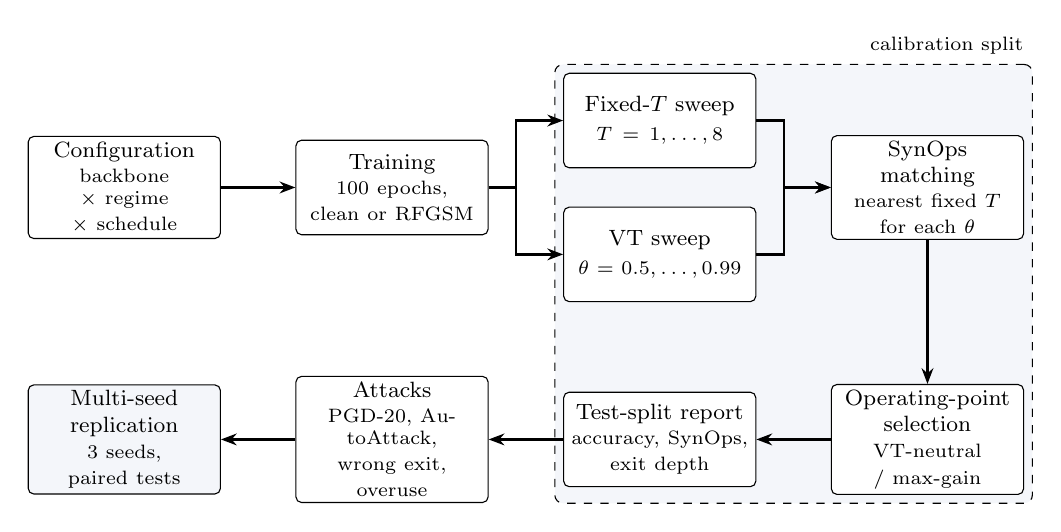
\begin{tikzpicture}[
        box/.style={draw, rounded corners=2pt, align=center, font=\footnotesize, minimum height=12mm, text width=23mm, inner sep=2pt, fill=white},
        grp/.style={draw, dashed, rounded corners=3pt, inner sep=3pt, fill=boxbg},
        arr/.style={-{Stealth[length=2mm]}, thick}
    ]
        \node[box] (cfg)   at (0, 0)       {Configuration\\[1pt]\scriptsize backbone $\times$ regime\\\scriptsize $\times$ schedule};
        \node[box] (train) at (3.4, 0)     {Training\\[1pt]\scriptsize 100 epochs,\\\scriptsize clean or RFGSM};
        \node[box] (fixed) at (6.8, 0.85)  {Fixed-$T$ sweep\\[1pt]\scriptsize $T = 1, \dots, 8$};
        \node[box] (vt)    at (6.8, -0.85) {VT sweep\\[1pt]\scriptsize $\theta = 0.5, \dots, 0.99$};
        \node[box] (match) at (10.2, 0)    {SynOps matching\\[1pt]\scriptsize nearest fixed $T$\\\scriptsize for each $\theta$};
        \node[box] (select) at (10.2, -3.2) {Operating-point\\selection\\\scriptsize VT-neutral / max-gain};
        \node[box] (test)   at (6.8, -3.2)  {Test-split report\\[1pt]\scriptsize accuracy, SynOps,\\\scriptsize exit depth};
        \node[box] (attack) at (3.4, -3.2)  {Attacks\\[1pt]\scriptsize PGD-20, AutoAttack,\\\scriptsize wrong exit, overuse};
        \node[box, fill=boxbg] (seeds) at (0, -3.2) {Multi-seed\\replication\\\scriptsize 3 seeds, paired tests};
        \begin{scope}[on background layer]
            \node[grp, fit=(fixed)(vt)(match)(select)] (cal) {};
        \end{scope}
        \node[font=\scriptsize, anchor=south east] at (cal.north east) {calibration split};
        \draw[arr] (cfg) -- (train);
        \draw[arr] (train.east) -- ++(0.35,0) |- (fixed.west);
        \draw[arr] (train.east) -- ++(0.35,0) |- (vt.west);
        \draw[arr] (fixed.east) -- ++(0.35,0) |- (match.west);
        \draw[arr] (vt.east) -- ++(0.35,0) |- (match.west);
        \draw[arr] (match) -- (select);
        \draw[arr] (select) -- (test);
        \draw[arr] (test) -- (attack);
        \draw[arr] (attack) -- (seeds);
    \end{tikzpicture}
    \caption[Overview of the experimental pipeline]{Overview of the experimental pipeline. Sweeps and operating-point selection use the calibration split, and all reported numbers use the test split.}
    \label{fig:pipeline}
\end{figure}

\section{Problem Formulation}
\label{sec:meth-formulation}

\subsection{Spiking neurons}

All networks in this thesis use deterministic leaky integrate-and-fire neurons. Let $I_t$ be the input current to a neuron at timestep $t$ (the output of the preceding convolution and batch normalisation), $V_t$ its membrane potential and $S_t \in \{0, 1\}$ its output spike. With time constant $\tau$ and firing threshold $V_\mathrm{th}$, the neuron is updated as
\begin{align}
    H_t &= V_{t-1} + \frac{1}{\tau}\left(I_t - V_{t-1}\right), \label{eq:lif-charge}\\
    S_t &= \Theta\left(H_t - V_\mathrm{th}\right), \label{eq:lif-fire}\\
    V_t &= H_t \left(1 - S_t\right), \label{eq:lif-reset}
\end{align}
where $\Theta$ is the Heaviside step function and $V_0 = 0$. \eqnref{eq:lif-charge} integrates the input with leak, \eqnref{eq:lif-fire} emits a spike when the charged potential reaches the threshold, and \eqnref{eq:lif-reset} resets the potential to zero after a spike (hard reset). We use $\tau = 2$ and $V_\mathrm{th} = 0.5$ throughout.

The derivative of $\Theta$ is replaced during backpropagation by the surrogate
\begin{equation}
    \frac{\partial S_t}{\partial H_t} \approx \frac{\alpha}{2\left(1 + \alpha \left|H_t - V_\mathrm{th}\right|\right)^2}, \qquad \alpha = 4,
    \label{eq:surrogate}
\end{equation}
and the reset term is detached from the computational graph, a common choice that improves training stability. Because the neurons are deterministic, the same input always produces the same spike train, so there is no stochastic component for an attacker to average over.

\subsection{Input encoding and readout}

We use direct encoding: the normalised image $x$ is fed to the first convolutional layer unchanged at every timestep, and the first layer of LIF neurons converts it into spikes. All subsequent layers communicate by spikes, except the final linear classifier, which produces real-valued logits $z_t \in \mathbb{R}^{K}$ at every timestep, with $K = 10$ classes.

The network's prediction after $t$ timesteps is based on the running mean of these logits,
\begin{equation}
    \bar{z}_t = \frac{1}{t} \sum_{s=1}^{t} z_s, \qquad \hat{y}_t = \arg\max_{k} \, \bar{z}_{t,k}.
    \label{eq:accum}
\end{equation}
Because the membrane potentials start at zero and need time to charge, the deep layers of the network emit few or no spikes at $t = 1$, and $\bar{z}_1$ is nearly independent of the input. As a result, fixed-horizon accuracy at $T = 1$ is at or near chance for most of our models (\tabref{tab:res-fixed}).

\subsection{Fixed-timestep inference}

Fixed-timestep inference with horizon $T$ runs every input for exactly $T$ timesteps and predicts $\hat{y}_T$. Its compute is the same for every input (up to differences in spike sparsity) and grows roughly linearly with $T$. Sweeping $T$ from 1 to 8 traces the fixed-timestep compute--accuracy curve, which serves as the baseline for VT.

\subsection{Variable timing}

Variable timing adds a stopping rule. Let $c(\cdot)$ map accumulated logits to a confidence score in $[0, 1]$, and let $\theta$ be a threshold. The exit time of input $x$ is
\begin{equation}
    \tau_\theta(x) = \min\left\{ t \in \{1, \dots, T_{\max}\} \;:\; c\left(\bar{z}_t(x)\right) \geq \theta \right\},
    \label{eq:exit}
\end{equation}
with $\tau_\theta(x) = T_{\max}$ if no such $t$ exists, and the VT prediction is $\hat{y}_{\tau_\theta(x)}$. We use $T_{\max} = 8$. The main stopping rule is the maximum softmax probability,
\begin{equation}
    c_{\mathrm{MSP}}(\bar{z}) = \max_{k} \operatorname{softmax}(\bar{z})_k,
    \label{eq:msp}
\end{equation}
which is the most common choice in the VT literature and a strong baseline in confidence estimation generally~\cite{hendrycks2017baseline}. Alternative rules are compared in \secref{sec:meth-stoprules}.

\figref{fig:vt-mechanism} illustrates the mechanism. After every timestep, the confidence of the accumulated prediction is compared with $\theta$. An easy input crosses the threshold early and exits, while a hard input continues until it crosses the threshold or reaches $T_{\max}$. The average exit depth $\mathbb{E}_x[\tau_\theta(x)]$ and the average compute fall as $\theta$ decreases.

\begin{figure}[htbp]
    \centering
    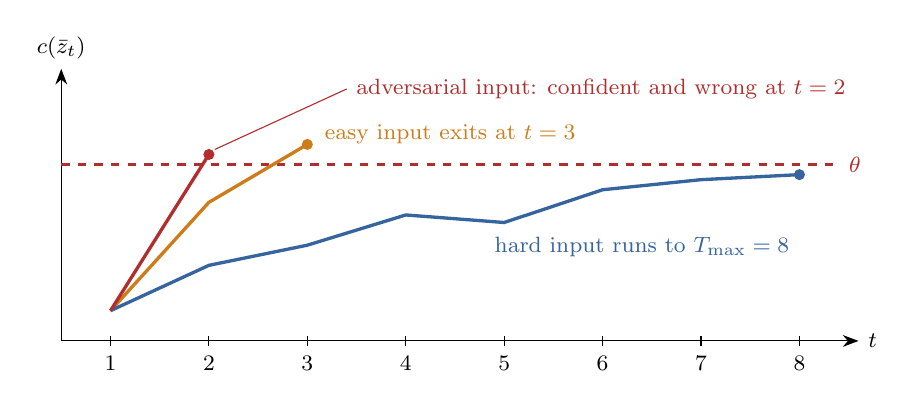
\begin{tikzpicture}[x=1.25cm, y=3.2cm, font=\footnotesize]
        \draw[-{Stealth[length=2mm]}] (0.5,0) -- (8.6,0) node[right] {$t$};
        \draw[-{Stealth[length=2mm]}] (0.5,0) -- (0.5,1.08) node[above] {$c(\bar{z}_t)$};
        \foreach \t in {1,...,8} \draw (\t,0.02) -- (\t,-0.02) node[below] {\t};
        \draw[dashed, catk, thick] (0.5,0.7) -- (8.4,0.7) node[right] {$\theta$};
        % easy input
        \draw[cvt, very thick] (1,0.12) -- (2,0.55) -- (3,0.78);
        \fill[cvt] (3,0.78) circle (2pt);
        \node[cvt, right] at (3.08,0.82) {easy input exits at $t=3$};
        % hard input
        \draw[cfix, very thick] (1,0.12) -- (2,0.3) -- (3,0.38) -- (4,0.5) -- (5,0.47) -- (6,0.6) -- (7,0.64) -- (8,0.66);
        \fill[cfix] (8,0.66) circle (2pt);
        \node[cfix, below] at (6.4,0.45) {hard input runs to $T_{\max}=8$};
        % attacked input
        \draw[catk, very thick] (1,0.12) -- (2,0.74);
        \fill[catk] (2,0.74) circle (2pt);
        \node[catk, right] (advlab) at (3.4,1.0) {adversarial input: confident and wrong at $t=2$};
        \draw[catk, thin] (2.06,0.76) -- (advlab.west);
    \end{tikzpicture}
    \caption[Variable-timing inference]{Variable-timing inference. The confidence of the accumulated prediction is checked after every timestep, and an input exits as soon as it reaches the threshold $\theta$. An adversary can try to make an input exit early with a wrong prediction (red), or to keep its confidence below $\theta$ so that it never exits early (\secref{sec:meth-attacks}).}
    \label{fig:vt-mechanism}
\end{figure}

\paragraph{Sample-exact execution.} In a batched implementation, a batch keeps running until all its inputs have exited, and exited inputs simply carry their frozen predictions. This does not change predictions, but it does change measured compute: a batch-level measurement charges every input for the slowest input's timesteps. We therefore measure compute with \emph{sample-exact} accounting, in which each input's synaptic operations are counted only up to its own exit time (\secref{sec:meth-synops}). The reported VT compute is exactly what a per-sample implementation on event-driven hardware would incur.

\section{Backbone Architectures}
\label{sec:meth-models}

We use spiking versions of three standard convolutional architectures, chosen to span a range of depth, width and parameter count. In every case, each ReLU of the original architecture is replaced by an LIF neuron (\eqnref{eq:lif-charge}--\eqref{eq:lif-reset}), and the final classifier is a real-valued linear layer. \tabref{tab:backbones} summarises them.

\begin{itemize}
    \item \textbf{ResNet-18}~\cite{he2016deep}, CIFAR variant: a $3\times3$ stem convolution with 64 channels followed by four stages of two basic residual blocks each with 64, 128, 256 and 512 channels, global average pooling and a linear classifier. LIF neurons follow every batch-normalised convolution, including on the shortcut path.
    \item \textbf{VGG16}~\cite{simonyan2015very}: thirteen $3\times3$ convolutions in five stages (2, 2, 3, 3 and 3 layers with 64, 128, 256, 512 and 512 channels), each followed by batch normalisation~\cite{ioffe2015batch} and an LIF neuron, with max pooling between stages and a classifier with two spiking hidden layers of 4096 units.
    \item \textbf{MobileNetV2}~\cite{sandler2018mobilenetv2}: inverted residual blocks with depthwise-separable convolutions in seven stages (16, 24, 32, 64, 96, 160 and 320 output channels with 1, 2, 3, 4, 3, 3 and 1 blocks), with LIF neurons replacing the ReLU6 activations.
\end{itemize}

\begin{table}[htbp]
    \centering
    \caption{Backbones used in this thesis. Dense operations are the multiply--accumulate operations a non-spiking network of the same shape would perform over eight timesteps, per image.}
    \label{tab:backbones}
    \small
    \begin{tabular}{@{}l r r r@{}}
        \toprule
        Backbone & Parameters & Dense ops at $T=8$ & Full-horizon SynOps (clean model) \\
        \midrule
        ResNet-18   & 11.2\,M & $4.44 \times 10^{9}$ & $4.14 \times 10^{8}$ \\
        VGG16       & 33.6\,M & $2.66 \times 10^{9}$ & $1.82 \times 10^{8}$ \\
        MobileNetV2 & 2.2\,M  & $0.70 \times 10^{9}$ & $3.77 \times 10^{8}$ \\
        \bottomrule
    \end{tabular}
\end{table}

The SynOps column of \tabref{tab:backbones} already shows the effect of spike sparsity: a spiking ResNet-18 at its full horizon performs fewer than a tenth of the operations of its dense counterpart, because most activations are zero at any given timestep. MobileNetV2, despite having the fewest dense operations, performs more synaptic operations than VGG16, because its depthwise and expansion layers are much less sparse.

\section{Training}
\label{sec:meth-training}

\subsection{Training regimes}

Every backbone is trained under two regimes.

\paragraph{Clean.} The model is trained on clean images with the cross-entropy loss $\mathcal{L}_{\mathrm{CE}}(f_T(x), y)$ of the accumulated logits after the training horizon $T$.

\paragraph{Adversarial.} The model is trained entirely on adversarial examples generated on the fly with FGSM from a random start (RFGSM)~\cite{tramer2018ensemble, wong2020fast}. For each training image, a random perturbation $\delta_0 \sim \mathcal{U}[-\gamma\epsilon, \gamma\epsilon]^d$ is drawn, a single signed gradient step is taken, and the result is projected onto the $\epsilon$-ball:
\begin{equation}
    x_{\mathrm{adv}} = \operatorname{clip}_{[0,1]}\!\left(x + \Pi_{\epsilon}\!\left[\delta_0 + \alpha \operatorname{sign}\!\left(\nabla_{\delta} \mathcal{L}_{\mathrm{CE}}\left(f_T(x + \delta_0), y\right)\right)\right]\right),
    \label{eq:rfgsm}
\end{equation}
with $\epsilon = \alpha = 8/255$ and $\gamma = 0.1$. The model is then updated on $\mathcal{L}_{\mathrm{CE}}(f_T(x_{\mathrm{adv}}), y)$ only, and no clean images are used.

The two regimes are deliberately pure: every checkpoint in this thesis was trained with a fixed clean fraction of exactly 0\% or 100\%, so that any difference between them can be attributed to the regime itself.

\subsection{Timestep schedules}

The training horizon is set by one of two schedules.

\paragraph{Fixed-T8.} Every training batch uses $T = 8$. This is the standard setting for directly trained SNNs and the schedule used for all three backbones.

\paragraph{Mixed-T.} For every training batch, $T$ is drawn uniformly from $\{1, \dots, 8\}$. Training at short horizons should make early predictions more useful, which matters for VT because VT relies on them. We train mixed-T models for ResNet-18 under both regimes to test this.

\subsection{Optimisation and hyperparameters}

All models are trained for 100 epochs with stochastic gradient descent (momentum 0.9, weight decay $10^{-4}$, base learning rate 0.1, batch size 256), with a linear warm-up over the first five epochs followed by cosine decay~\cite{loshchilov2017sgdr}. We use automatic mixed precision with float16~\cite{micikevicius2018mixed} and clip the gradient norm at 1.0. Training images are augmented with random cropping (4-pixel padding), horizontal flipping and Cutout~\cite{devries2017improved} with one $16\times16$ hole. Clean validation accuracy at the full horizon is evaluated every five epochs, and the checkpoint with the highest validation accuracy is kept. \tabref{tab:app-hparams} in Appendix~\ref{app:hparams} lists every hyperparameter.

\subsection{Model configurations}

\tabref{tab:configs} lists the nine trained configurations. ResNet-18 is the primary backbone: it is trained under both regimes and both schedules, and the adversarial fixed-T8 configuration was trained twice with identical settings. VGG16 and MobileNetV2 are trained with the fixed-T8 schedule under both regimes.

\begin{table}[htbp]
    \centering
    \caption{Model configurations. The short names are used in the results tables and figures.}
    \label{tab:configs}
    \small
    \begin{tabular}{@{}l l l l l@{}}
        \toprule
        Short name & Backbone & Regime & Schedule & Note \\
        \midrule
        R18 clean        & ResNet-18   & Clean       & Fixed-T8 & \\
        R18 adv (1)      & ResNet-18   & Adversarial & Fixed-T8 & first run \\
        R18 adv (2)      & ResNet-18   & Adversarial & Fixed-T8 & identical re-run \\
        R18 clean mixT   & ResNet-18   & Clean       & Mixed-T  & \\
        R18 adv mixT     & ResNet-18   & Adversarial & Mixed-T  & \\
        VGG clean        & VGG16       & Clean       & Fixed-T8 & \\
        VGG adv          & VGG16       & Adversarial & Fixed-T8 & \\
        MBv2 clean       & MobileNetV2 & Clean       & Fixed-T8 & \\
        MBv2 adv         & MobileNetV2 & Adversarial & Fixed-T8 & \\
        \bottomrule
    \end{tabular}
\end{table}

\section{Data and Splits}
\label{sec:meth-data}

All experiments use CIFAR-10~\cite{krizhevsky2009learning}: 50{,}000 training and 10{,}000 test images of size $32 \times 32$ in ten classes. We split the official training set with a fixed seed into three disjoint parts (\figref{fig:splits}): 40{,}000 images for training, 5{,}000 for validation (checkpoint selection) and 5{,}000 for calibration (threshold sweeps and operating-point selection). The 10{,}000 test images are used only for reporting. Separating calibration from test ensures that the operating point is chosen without looking at the data on which it is reported.

Adversarial evaluation is expensive, so attacks are run on a class-balanced subset of the test set: 2{,}000 images (200 per class) for the single-run experiments and 1{,}000 images (100 per class) for the multi-seed experiments, drawn with a fixed seed. The earliest ResNet-18 experiments were attacked on the full test set, which is noted where relevant.

\begin{figure}[htbp]
    \centering
    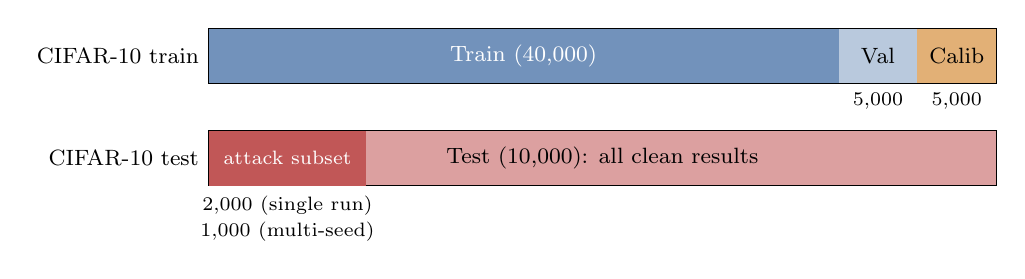
\begin{tikzpicture}[font=\footnotesize]
        \def\h{0.7}
        \fill[cfix!70] (0,0) rectangle (8,\h);
        \fill[cfix!35] (8,0) rectangle (9,\h);
        \fill[cvt!60] (9,0) rectangle (10,\h);
        \draw (0,0) rectangle (10,\h);
        \node[white] at (4,\h/2) {Train (40{,}000)};
        \node at (8.5,\h/2) {Val};
        \node at (9.5,\h/2) {Calib};
        \node[below] at (8.5,0) {\scriptsize 5{,}000};
        \node[below] at (9.5,0) {\scriptsize 5{,}000};
        \node[left] at (0,\h/2) {CIFAR-10 train};
        \fill[catk!45] (0,-1.3) rectangle (10,-1.3+\h);
        \draw (0,-1.3) rectangle (10,-1.3+\h);
        \node at (5,-1.3+\h/2) {Test (10{,}000): all clean results};
        \fill[catk!80] (0,-1.3) rectangle (2,-1.3+\h);
        \node[white] at (1,-1.3+\h/2) {\scriptsize attack subset};
        \node[left] at (0,-1.3+\h/2) {CIFAR-10 test};
        \node[below, align=center] at (1,-1.3) {\scriptsize 2{,}000 (single run)\\\scriptsize 1{,}000 (multi-seed)};
    \end{tikzpicture}
    \caption[Data splits]{Data splits. Training uses 40{,}000 images. Checkpoints are selected on validation, operating points on calibration, and all results are reported on test. Attacks use a class-balanced test subset.}
    \label{fig:splits}
\end{figure}

\section{Compute Accounting}
\label{sec:meth-synops}

We measure compute in synaptic operations. For a convolutional or linear layer $\ell$ executed at timestep $t$, let $D_\ell$ be the number of multiply--accumulate operations a dense execution would perform and $\rho_{\ell,t}(x)$ the fraction of the layer's input activations that are non-zero. The synaptic operations of the layer are $D_\ell \, \rho_{\ell,t}(x)$: only non-zero inputs trigger work. For an input that runs for $\tau(x)$ timesteps,
\begin{equation}
    \SynOps(x) = \sum_{t=1}^{\tau(x)} \sum_{\ell} D_\ell \, \rho_{\ell,t}(x),
    \label{eq:synops}
\end{equation}
and we report the mean over the evaluation set. For the first layer, whose input is the real-valued image, $\rho = 1$, so its dense cost is counted in full at every timestep. For fixed-timestep inference $\tau(x) = T$, and for VT $\tau(x) = \tau_\theta(x)$, measured per sample. SynOps is a hardware-independent proxy: it captures the effect of both sparsity and exit depth, but not memory access or membrane-update costs~\cite{dampfhoffer2023snns}. We use it to compare VT and fixed-timestep inference on the same network, where those omitted costs scale similarly with the number of timesteps run.

\section{Compute-Matched Evaluation Protocol}
\label{sec:meth-protocol}

For each trained model, we run two sweeps on the calibration split and repeat them on the test split:

\begin{itemize}
    \item a \emph{fixed sweep} at $T \in \{1, \dots, 8\}$, recording accuracy and mean SynOps, and
    \item a \emph{VT sweep} at $\theta \in \Theta = \{0.5, 0.6, 0.7, 0.8, 0.85, 0.9, 0.95, 0.99\}$, recording accuracy, mean exit depth, the histogram of exit times and mean SynOps.
\end{itemize}

Each VT point $\theta$ is then paired with its \emph{compute-matched control}: the fixed horizon whose mean SynOps is closest to that of VT at $\theta$,
\begin{equation}
    T^{*}(\theta) = \arg\min_{T \in \{1,\dots,8\}} \left| \SynOps_{\VT}(\theta) - \SynOps_{\mathrm{fix}}(T) \right|.
    \label{eq:match}
\end{equation}
The \emph{gain} of VT at $\theta$ is its accuracy minus that of the matched control,
\begin{equation}
    \Delta(\theta) = \mathrm{Acc}_{\VT}(\theta) - \mathrm{Acc}_{\mathrm{fix}}\left(T^{*}(\theta)\right).
    \label{eq:gain}
\end{equation}
A positive gain means that, for roughly the same compute, choosing when to stop per input is better than stopping every input at the same time. Because the fixed horizons are discrete, the match is approximate. We report both SynOps values so that the residual mismatch is visible, and we additionally report whether each VT point lies above the piecewise-linear fixed-timestep frontier.

We also report VT against the \emph{full-horizon} model ($T = 8$). This comparison answers a different question, namely what VT gives up relative to running the whole budget, and both are needed to interpret the robustness results.

\section{Operating-Point Selection}
\label{sec:meth-selection}

Every reported VT result is at some threshold, and the threshold must be selected without looking at test data. We consider two selection rules, both applied to the calibration sweeps.

\paragraph{Max-gain selection.} The rule used in our original experiments selects the threshold with the largest gain over its matched control on the calibration split, $\hat\theta_{\mathrm{gain}} = \arg\max_{\theta} \Delta_{\mathrm{cal}}(\theta)$. This rule is natural, since it picks the point where VT looks best, but it is \emph{biased} in favour of VT: it rewards VT on exactly the comparison it is being evaluated on, and it can prefer points where both VT and its control are poor, as long as the control is poorer. We show in \secref{sec:res-selection} that this happens in practice.

\paragraph{VT-neutral selection.} The alternative rule ignores the matched control entirely. Given a tolerance $\delta$, it selects the cheapest threshold whose calibration accuracy is within $\delta$ points of the full-horizon accuracy:
\begin{equation}
    \hat\theta_{\delta} = \arg\min_{\theta \in \Theta} \left\{ \SynOps_{\VT,\mathrm{cal}}(\theta) \;:\; \mathrm{Acc}_{\VT,\mathrm{cal}}(\theta) \geq \mathrm{Acc}_{\mathrm{fix},\mathrm{cal}}(8) - \delta \right\}.
    \label{eq:neutral}
\end{equation}
If no threshold meets the tolerance, the most accurate threshold is chosen. This is the rule a practitioner would actually use: decide how much accuracy one is willing to give up, then take the cheapest setting that meets it. Because it never looks at the fixed-timestep controls, it cannot favour VT in the comparison with them. \algref{alg:neutral} gives the full procedure. We use $\delta = 1$ point as the primary setting and report $\delta \in \{0.5, 2\}$ as a sensitivity analysis.

\begin{algorithm}[htbp]
    \caption{VT-neutral operating-point selection and compute-matched reporting}
    \label{alg:neutral}
    \begin{algorithmic}[1]
        \Require trained model $f$; threshold grid $\Theta$; tolerance $\delta$; calibration set $\mathcal{D}_{c}$; test set $\mathcal{D}_{t}$
        \For{$T = 1, \dots, 8$} \Comment{fixed sweep}
            \State $(a^{c}_T, s^{c}_T) \gets$ accuracy and mean SynOps of $f$ at horizon $T$ on $\mathcal{D}_c$
        \EndFor
        \For{$\theta \in \Theta$} \Comment{VT sweep, sample-exact}
            \State $(v^{c}_\theta, u^{c}_\theta) \gets$ accuracy and mean SynOps of VT$(f, \theta)$ on $\mathcal{D}_c$
        \EndFor
        \State $\mathcal{C} \gets \{\theta \in \Theta : v^{c}_\theta \geq a^{c}_8 - \delta\}$
        \If{$\mathcal{C} = \emptyset$}
            \State $\hat\theta \gets \arg\max_\theta v^{c}_\theta$ \Comment{fallback}
        \Else
            \State $\hat\theta \gets \arg\min_{\theta \in \mathcal{C}} u^{c}_\theta$
        \EndIf
        \State Evaluate VT$(f, \hat\theta)$ and fixed $T = 1..8$ on $\mathcal{D}_t$
        \State $T^{*} \gets \arg\min_T |u^{t}_{\hat\theta} - s^{t}_T|$ \Comment{compute-matched control}
        \State \Return $v^{t}_{\hat\theta} - a^{t}_{T^*}$, \; $v^{t}_{\hat\theta} - a^{t}_8$, \; $u^{t}_{\hat\theta} / s^{t}_8$
    \end{algorithmic}
\end{algorithm}

\paragraph{Which rule was used where.} The clean-data results in this thesis are recomputed from the saved calibration and test sweeps under both rules, which requires no new model evaluations. The attack experiments, however, were run at the thresholds chosen by the max-gain rule (with one manual override, noted in \secref{sec:res-selection}), together with their immediate neighbours in $\Theta$. Re-running them at the VT-neutral thresholds was not possible within our compute budget. For the adversarially trained models, the two rules select the same or adjacent thresholds (\tabref{tab:res-selection}), so this affects the clean-trained robustness results most, and those are near zero under every rule.

\section{Stopping Rules}
\label{sec:meth-stoprules}

To test whether the conclusions depend on the choice of confidence score, we compare five stopping rules, each computed on the accumulated logits $\bar{z}_t$ with $p = \operatorname{softmax}(\bar{z}_t)$:

\begin{itemize}
    \item \textbf{Max softmax}: $c = \max_k p_k$ (the primary rule, \eqnref{eq:msp}).
    \item \textbf{Margin}: $c = p_{(1)} - p_{(2)}$, the difference between the two largest probabilities.
    \item \textbf{Entropy}: $c = 1 - H(p) / \log K$, one minus the normalised predictive entropy.
    \item \textbf{Temperature softmax}: $c = \max_k \operatorname{softmax}(\bar{z}_t / 2)_k$, MSP with temperature 2.
    \item \textbf{Evidential surrogate}: with $\alpha_k = \operatorname{softplus}(\bar{z}_{t,k}) + 1$, $c = 1 - K / \sum_k \alpha_k$, one minus the Dirichlet uncertainty mass~\cite{sensoy2018evidential}.
\end{itemize}

Because the rules have different scales, comparing them at the same $\theta$ is meaningless. Instead, for each rule we choose the threshold whose mean exit depth on the calibration split is closest to that of the max-softmax operating point, and compare test accuracy at (approximately) equal depth. A rule that is better at identifying inputs that are already correctly classified will achieve higher accuracy at the same depth.

\section{Threat Model and Attacks}
\label{sec:meth-attacks}

\subsection{Threat model}

We consider a white-box adversary who knows the model weights, the stopping rule and the threshold, and who perturbs each test image within an $\ell_\infty$ ball of radius $\epsilon = 8/255$, keeping pixel values in $[0, 1]$. The adversary has one of three goals:

\begin{enumerate}
    \item \textbf{Misclassification}: make the final prediction wrong (untargeted attack).
    \item \textbf{Wrong early exit}: make the input exit early with a wrong prediction.
    \item \textbf{Compute overuse}: keep the prediction \emph{correct} but delay the exit, increasing the compute spent on the input.
\end{enumerate}

The first goal is the standard robustness setting. The second and third are specific to VT and target its exit gate.

\subsection{Attacking through the exit gate}

The exit decision in \eqnref{eq:exit} is a hard threshold, so it has no gradient. An attacker who differentiates only through the full-horizon output $\bar{z}_8$ is attacking a different function from the one being deployed. We therefore give the attacker the full trace: for each candidate perturbation, the network is run for all eight timesteps, the exit time $\tau_\theta(x)$ is determined from the per-timestep confidences, and the loss is computed on the accumulated logits $\bar{z}_{\tau_\theta(x)}$ at the actual exit step. Gradients flow through those logits and through all earlier timesteps' spiking dynamics, but not through the choice of exit step itself. This is an adaptive attack in the sense of Tram\`er et al.~\cite{tramer2020adaptive}: it attacks the deployed decision rule, not a proxy. Because our neurons are deterministic, no Expectation over Transformation is needed.

\subsection{Misclassification attacks}

\paragraph{PGD-20.} Projected gradient descent~\cite{madry2018towards} with 20 iterations, step size $2/255$, a uniform random start in the $\epsilon$-ball and the cross-entropy loss on the exit-step logits.

\paragraph{AutoAttack.} The standard version of AutoAttack~\cite{croce2020reliable}: APGD-CE, APGD-T, FAB-T~\cite{croce2020minimally} and Square~\cite{andriushchenko2020square}, applied in sequence, each to the images that the previous attacks failed to break. The model is wrapped so that AutoAttack sees the VT decision rule through the exit-step logits as above.

Each attack is applied to three inference modes on the same images: the full-horizon model ($T = 8$), the compute-matched fixed horizon $T^{*}$, and VT at the selected threshold. The fixed-mode models are attacked through their own $T$-step outputs.

\subsection{Gate-specific attacks}

Both gate-specific attacks use PGD with the same budget as PGD-20 but a different loss computed over the whole trace. Let $m_t(x) = \max_{k \neq y} \bar{z}_{t,k} - \bar{z}_{t,y}$ be the misclassification margin of the accumulated logits at step $t$ (positive when the prediction is wrong) and $c_t = c(\bar{z}_t)$ the confidence.

\paragraph{Wrong early exit.} The attacker maximises a weighted sum of margin and confidence that emphasises early timesteps,
\begin{equation}
    \mathcal{L}_{\mathrm{early}} = \frac{1}{T_{\max}} \sum_{t=1}^{T_{\max}} w_t \left( m_t + \lambda_{\mathrm{c}} \, c_t \right), \qquad w_t = \frac{T_{\max} - t + 1}{T_{\max}},
    \label{eq:wrong-exit}
\end{equation}
with $\lambda_{\mathrm{c}} = 0.25$, encouraging predictions that are wrong and confident as early as possible.

\paragraph{Compute overuse.} The attacker maximises the normalised entropy $\tilde{H}_t$ and minimises the confidence of the accumulated prediction at every timestep, while preserving the correct final label:
\begin{equation}
    \mathcal{L}_{\mathrm{overuse}} = \frac{1}{T_{\max}} \sum_{t=1}^{T_{\max}} \left(\tilde{H}_t - c_t\right) \; - \; \lambda_{\mathrm{p}} \, \mathcal{L}_{\mathrm{CE}}\left(\bar{z}_{\tau}, y\right),
    \label{eq:overuse}
\end{equation}
with $\lambda_{\mathrm{p}} = 1$. The first term pushes confidence below the threshold so that the input does not exit, and the second keeps the prediction correct, so that the attack is invisible to anyone monitoring accuracy. We report the increase in mean exit depth (depth inflation) and the fraction of attacked inputs that are still correctly classified. This attack is the SNN analogue of slowdown attacks on multi-exit networks~\cite{hong2021panda} and of sponge examples~\cite{shumailov2021sponge}.

\subsection{Attack variance}

For one checkpoint per adversarially trained backbone, PGD-20 and AutoAttack were repeated with three attack seeds (different random starts, and different random choices inside AutoAttack). The standard deviation across attack seeds was at most 1.74 points for every mode and backbone (\tabref{tab:app-attack-seed}), much smaller than the training-seed variance, so the remaining experiments use a single attack seed.

\section{Multi-Seed Replication and Statistical Analysis}
\label{sec:meth-stats}

\subsection{Multi-seed design}

Single-run results can be dominated by training variance. To test which conclusions replicate, the adversarially trained fixed-T8 configurations were re-trained from scratch with three seeds ($s \in \{0, 1, 2\}$) for ResNet-18 and VGG16, using the same pure-adversarial regime as the single-run models. For each seed, the operating point and its compute-matched control were selected on the calibration split, and clean accuracy, PGD-20 and AutoAttack were measured for the full-horizon, matched and VT modes on the same 1{,}000-image balanced test subset. A MobileNetV2 multi-seed run was also started but exceeded the 12-hour Kaggle session limit before its evaluations completed, so only its training histories and attack-seed variance are available.

The multi-seed notebooks select operating points with the max-gain rule and save only the selected point, not the full sweeps, so they cannot be re-selected with the VT-neutral rule. The selected points are nevertheless sensible: for every seed, the VT point is within about three points of the full-horizon accuracy on clean data, and the matched horizons ($T^* = 5$ for ResNet-18, $T^* = 6$ for VGG16) are the same as those of the single-run VT-neutral points.

\subsection{Paired differences}

All comparisons are \emph{paired}: VT, its matched control and the full-horizon model are evaluated on the same checkpoint and the same images, and we analyse the per-checkpoint difference $d_s = \mathrm{Acc}_{\VT,s} - \mathrm{Acc}_{\mathrm{ref},s}$. Pairing removes the variation between checkpoints, which is large (up to 7 points in full-horizon AutoAttack accuracy across our ResNet-18 seeds), and isolates the effect of the inference mode~\cite{bouthillier2021accounting}.

\subsection{Tests}

For each comparison and metric we report the mean and sample standard deviation of $d_s$ over checkpoints, the number of checkpoints with $d_s > 0$, and two tests of the null hypothesis that the mean difference is zero:

\begin{itemize}
    \item a one-sample $t$-test on $\{d_s\}$, with $t = \bar{d} / (s_d / \sqrt{n})$ and $n - 1$ degrees of freedom, and
    \item an exact two-sided sign test (binomial test on the number of positive differences), which makes no distributional assumption.
\end{itemize}

We pool the three ResNet-18 and three VGG16 seeds ($n = 6$) for the main tests and also report each backbone separately. With so few checkpoints these tests have limited power: a non-significant result means the data do not distinguish the difference from zero, not that the difference is zero. We therefore interpret them together with the sign of every individual seed.

For single-run accuracies on $n$ images, we report the binomial 95\% confidence half-width $1.96 \sqrt{p(1-p)/n}$ as a guide to evaluation noise: about $\pm 0.6$--$1.0$ points for clean accuracy on the 10{,}000-image test set and about $\pm 2$ points for attacked accuracy on a 2{,}000-image subset. This captures only test-sampling noise. Training-seed variance, which is larger, is addressed by the multi-seed experiments.

\section{Implementation and Reproducibility}
\label{sec:meth-impl}

\paragraph{Code base.} The experimental suite is written in PyTorch~\cite{paszke2019pytorch}. It descends from the BrainCog implementation of RandHet-SNN~\cite{wang2025random}, from which we retain the data pipeline and training scaffolding. We replaced the stochastic heterogeneous neurons with deterministic LIF neurons, removed the noise-scaling, Parseval and weight-perturbation components, and added the VT inference path with per-step traces, sample-exact compute accounting, the stopping rules, the compute-matched evaluation protocol, the gate-specific attacks and the multi-seed analysis. AutoAttack is run through the torchattacks library~\cite{kim2020torchattacks}, with the reference AutoAttack implementation as a fallback.

\paragraph{Execution environment.} All training and evaluation ran on Kaggle GPU sessions with internet access disabled. CIFAR-10 and the attack libraries were attached as offline datasets. Each experiment is a self-contained notebook generated by a builder script, so that the exact code that produced a result is preserved alongside it. Mixed precision, TF32 matrix multiplication and cuDNN autotuning were enabled for speed.

\paragraph{Analysis.} Every number in \chapref{ch:results} is computed by an analysis script from the raw CSV files written by the notebooks, and the script also writes a facts sheet that the text was checked against. Figures are generated from the same data. Appendix~\ref{app:repro} lists the files and the commands to regenerate them.

\section{Summary}

We study variable timing in deterministic LIF SNNs on CIFAR-10 across three backbones, two training regimes and two timestep schedules. Every VT operating point is compared with the fixed horizon of nearest measured compute, using sample-exact SynOps, and selected on a calibration split with a rule that does not favour VT. Robustness is measured with PGD-20 and AutoAttack by an attacker who differentiates through the exit-step logits, and two further attacks target the exit gate directly. Key comparisons are replicated across three training seeds and analysed with paired tests. The next chapter presents the results.

\chapter{Results and Discussion}
\label{ch:results}

This chapter presents the experimental results. \secref{sec:res-map} maps the experiments to the research questions and \secref{sec:res-setup} summarises the setup and metrics. \secref{sec:res-fixed} characterises fixed-timestep inference, the baseline against which everything else is measured. \secref{sec:res-efficiency} answers RQ1 on clean data, \secref{sec:res-stoprules} tests whether the answer depends on the stopping rule, and \secref{sec:res-selection} shows how it depends on the operating-point selection rule (RQ4). \secref{sec:res-robustness} turns to robustness (RQ2), \secref{sec:res-gate} to the gate-specific attacks (RQ3), and \secref{sec:res-multiseed} to the multi-seed replication that decides which of these findings hold. \secref{sec:res-discussion} discusses the results together, and \secref{sec:res-threats} examines threats to validity.

\section{Mapping Objectives to Experiments}
\label{sec:res-map}

\tabref{tab:res-map} lists the experiments, the research questions they address and where their results appear.

\begin{table}[htbp]
    \centering
    \caption{Experiments, the research questions they address, and where their results are reported.}
    \label{tab:res-map}
    \small
    \begin{tabularx}{\textwidth}{@{}>{\raggedright\arraybackslash}X l l l@{}}
        \toprule
        Experiment & RQ & Configurations & Section \\
        \midrule
        Fixed-timestep sweeps $T = 1..8$                       & ---      & all 9                 & \ref{sec:res-fixed} \\
        VT sweeps and compute-matched comparison               & RQ1      & all 9                 & \ref{sec:res-efficiency} \\
        Fixed-T8 vs mixed-T training schedule                  & RQ1      & ResNet-18 (4)         & \ref{sec:res-mixt} \\
        Stopping-rule comparison at matched depth              & RQ1, RQ4 & 7 of 9                & \ref{sec:res-stoprules} \\
        Max-gain vs VT-neutral selection; tolerance $\delta$   & RQ4      & all 9                 & \ref{sec:res-selection} \\
        PGD-20 and AutoAttack, single run                      & RQ2      & all 9                 & \ref{sec:res-robustness} \\
        Confidence trajectories under attack                   & RQ2, RQ3 & ResNet-18 adv         & \ref{sec:res-probe} \\
        Wrong-early-exit and compute-overuse attacks           & RQ3      & all 9                 & \ref{sec:res-gate} \\
        Three-seed replication with paired tests               & RQ1, RQ2, RQ4 & ResNet-18, VGG16 adv & \ref{sec:res-multiseed} \\
        Attack-seed variance                                   & RQ4      & 3 adv backbones       & \ref{sec:res-multiseed} \\
        \bottomrule
    \end{tabularx}
\end{table}

\section{Setup and Metrics}
\label{sec:res-setup}

The setup is described in full in \chapref{ch:method}, and here we summarise the points needed to read the results. All models are spiking LIF networks with $T_{\max} = 8$, trained for 100 epochs on 40{,}000 CIFAR-10 images. Operating points are selected on a 5{,}000-image calibration split and reported on the 10{,}000-image test set. Attacks are $\ell_\infty$ with $\epsilon = 8/255$, run on a 2{,}000-image class-balanced test subset (1{,}000 for the multi-seed study). We report:

\begin{itemize}
    \item \textbf{Accuracy} (\%) on clean or attacked inputs.
    \item \textbf{Mean SynOps} per image (\eqnref{eq:synops}), and the \textbf{SynOps saving} of VT relative to the full horizon, $1 - \SynOps_{\VT} / \SynOps_{\mathrm{fix}}(8)$.
    \item \textbf{Mean exit depth}: the average number of timesteps executed.
    \item \textbf{Gain}: VT accuracy minus the accuracy of the compute-matched fixed horizon $T^*$ (\eqnref{eq:gain}).
    \item \textbf{Below full}: full-horizon accuracy minus VT accuracy, i.e.\ what VT gives up relative to running all eight timesteps.
\end{itemize}

All differences are in percentage points (``points''). As a guide, the binomial 95\% half-width is $\pm 0.6$--$1.0$ points for clean accuracy on the full test set and about $\pm 2$ points for attacked accuracy on a 2{,}000-image subset.

\section{Fixed-Timestep Behaviour}
\label{sec:res-fixed}

\tabref{tab:res-fixed} and \figref{fig:fixed-sweeps} show test accuracy as a function of the fixed horizon $T$ for all nine configurations. Four observations shape the rest of the chapter.

\begin{table}[htbp]
    \centering
    \caption{Clean test accuracy (\%) of fixed-timestep inference at each horizon $T$ ($n = 10{,}000$).}
    \label{tab:res-fixed}
    \small
    \setlength{\tabcolsep}{5pt}
    \begin{tabular}{@{}l r r r r r r r r@{}}
        \toprule
        Configuration & $T=1$ & 2 & 3 & 4 & 5 & 6 & 7 & 8 \\
        \midrule
        R18 clean       & 10.00 & 84.72 & 87.89 & 90.11 & 90.48 & 90.97 & 91.09 & 91.26 \\
        R18 adv (1)     & 12.11 & 57.51 & 66.79 & 69.35 & 71.46 & 72.98 & 73.23 & 73.67 \\
        R18 adv (2)     & 10.00 & 58.74 & 65.93 & 72.30 & 73.53 & 76.01 & 76.32 & 77.18 \\
        R18 clean mixT  & 41.39 & 81.48 & 86.75 & 88.78 & 89.80 & 90.26 & 90.61 & 90.57 \\
        R18 adv mixT    & 46.28 & 70.04 & 74.31 & 76.26 & 76.82 & 77.14 & 77.58 & 77.79 \\
        VGG clean       & 10.00 & 70.94 & 80.50 & 84.63 & 86.16 & 87.50 & 87.82 & 88.20 \\
        VGG adv         & 10.00 & 23.81 & 51.41 & 57.62 & 61.23 & 63.75 & 64.62 & 65.52 \\
        MBv2 clean      & 10.00 & 17.60 & 37.72 & 61.06 & 64.91 & 73.92 & 74.71 & 77.66 \\
        MBv2 adv        & 10.00 & 23.47 & 36.55 & 45.54 & 47.63 & 50.09 & 50.64 & 51.44 \\
        \bottomrule
    \end{tabular}
\end{table}

\begin{figure}[htbp]
    \centering
    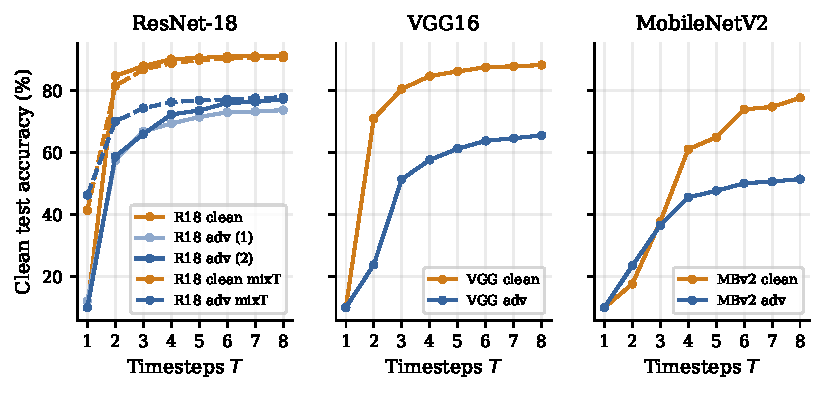
\includegraphics[width=\textwidth]{fixed_sweeps}
    \caption[Fixed-timestep accuracy as a function of the horizon]{Clean test accuracy of fixed-timestep inference as a function of the horizon $T$. Solid lines show the fixed-T8 training schedule and dashed lines the mixed-T schedule.}
    \label{fig:fixed-sweeps}
\end{figure}

\paragraph{The first timestep carries no information for fixed-T8 models.} Every model trained only at $T = 8$ is at chance (10\%) at $T = 1$. With $V_0 = 0$, a leak of $1/\tau = 1/2$ and a threshold of $0.5$, deep-layer neurons cannot reach threshold in a single step, so the output at $t = 1$ is essentially the classifier bias. Mixed-T models, which were trained to produce useful predictions at $T = 1$, reach 41--46\% there.

\paragraph{Accuracy saturates, but at different rates.} ResNet-18 clean reaches 87.89\% at $T = 3$, within 3.4 points of its $T = 8$ accuracy. VGG16 clean needs $T = 5$ to come within about two points, and MobileNetV2 needs $T = 6$--$8$. Adversarially trained models saturate more slowly than their clean counterparts on every backbone. How quickly a backbone saturates bounds how much any early-exit method can save: if the fixed-timestep curve is flat after $T = 3$, there is little to gain by stopping at $T = 3$ for some inputs and $T = 8$ for others.

\paragraph{Adversarial training costs 14--26 points of clean accuracy.} At $T = 8$, adversarial training reduces clean accuracy from 91.26\% to 73.67--77.18\% on ResNet-18, from 88.20\% to 65.52\% on VGG16 and from 77.66\% to 51.44\% on MobileNetV2, consistent with the robustness--accuracy trade-off reported for ANNs~\cite{tsipras2019robustness}. MobileNetV2 is the weakest backbone in both regimes, and its depthwise layers appear to suffer most from binarised activations.

\paragraph{Mixed-T training reshapes the curve.} The effect of the mixed-T schedule depends on the regime. Under adversarial training it improves accuracy at every horizon, by up to 11 points at $T = 2$. Under clean training it lifts only $T = 1$ (41.39\% vs 10.00\%) and is slightly \emph{worse} at every other horizon (for example 86.75\% vs 87.89\% at $T = 3$). Full-horizon accuracy is roughly unchanged in both regimes (90.57\% vs 91.26\% clean, 77.79\% vs 77.18\% adversarial). It also changes sparsity: the mixed-T clean ResNet-18 performs $5.65 \times 10^{8}$ SynOps at $T = 8$, 37\% more than its fixed-T8 counterpart ($4.14 \times 10^{8}$), because its neurons fire more. We return to the consequences for VT in \secref{sec:res-mixt}.

\section{RQ1: Efficiency at Equal Compute}
\label{sec:res-efficiency}

\subsection{The compute--accuracy frontier}

\figref{fig:frontier-main} shows the VT and fixed-timestep frontiers for the clean-trained ResNet-18, our primary configuration. Each orange point is one VT threshold and each blue point is one fixed horizon. At every compute level, the VT curve lies above the fixed-timestep curve. At the VT-neutral operating point ($\theta = 0.90$, $\delta = 1$), VT reaches 90.62\% with a mean exit depth of 3.01 timesteps and $1.33 \times 10^{8}$ SynOps per image. The compute-matched fixed horizon, $T^* = 3$, uses $1.27 \times 10^{8}$ SynOps and reaches 87.89\%. VT is therefore 2.73 points more accurate at slightly more than the same compute, and only 0.64 points below the full-horizon model while using 68\% fewer SynOps.

\begin{figure}[htbp]
    \centering
    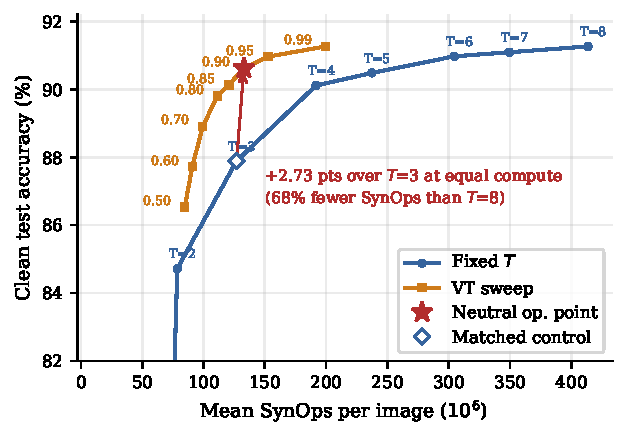
\includegraphics[width=0.8\textwidth]{frontier_r18_clean}
    \caption[Compute--accuracy frontier for the clean-trained ResNet-18]{Compute--accuracy frontier for the clean-trained ResNet-18 (test set). Orange: VT at each threshold $\theta$. Blue: fixed-timestep inference at each horizon. The star marks the VT-neutral operating point and the diamond its compute-matched fixed-timestep control.}
    \label{fig:frontier-main}
\end{figure}

\figref{fig:frontiers-all} repeats the comparison for all nine configurations, and \tabref{tab:res-neutral} lists the VT-neutral operating points. The pattern is consistent: \textbf{at the VT-neutral operating point, VT is more accurate than its compute-matched fixed horizon on all nine configurations}, with gains from $+0.14$ to $+3.37$ points.

\begin{figure}[htbp]
    \centering
    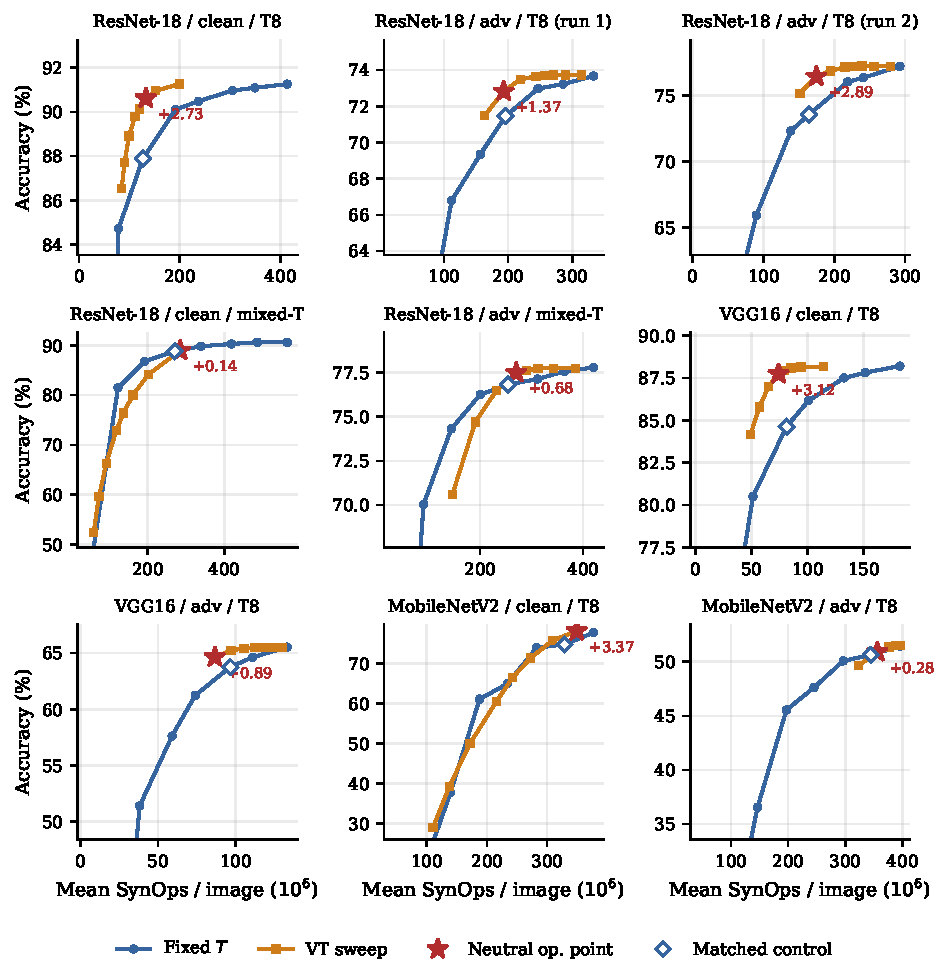
\includegraphics[width=\textwidth]{frontiers_all}
    \caption[Compute--accuracy frontiers for all configurations]{Compute--accuracy frontiers for all nine configurations (test set). Annotations give the gain of the VT-neutral operating point ($\delta = 1$) over its compute-matched control. The $y$-axes are cropped to the region of interest, so fixed-timestep points at $T = 1$ (and $T = 2$ where far below) lie off the bottom of several panels.}
    \label{fig:frontiers-all}
\end{figure}

\begin{table}[htbp]
    \centering
    \caption[VT-neutral operating points]{VT-neutral operating points ($\delta = 1$, selected on calibration, reported on test, $n = 10{,}000$). Depth: mean exit timestep. $T^*$: compute-matched fixed horizon. Gain: VT minus matched fixed accuracy. Below full: $T=8$ accuracy minus VT accuracy. Saving: SynOps saved relative to $T = 8$. Above: number of VT thresholds (of 8) that lie above the fixed-timestep frontier. $^\dagger$No threshold met the tolerance, so the most accurate was used.}
    \label{tab:res-neutral}
    \small
    \setlength{\tabcolsep}{4pt}
    \begin{tabular}{@{}l c c r c r r r r c@{}}
        \toprule
        Configuration & $\theta$ & Depth & VT acc & $T^*$ & Fixed acc & Gain & Below full & Saving & Above \\
        \midrule
        R18 clean                 & 0.90 & 3.01 & 90.62 & 3 & 87.89 & $+2.73$ & 0.64 & 67.9\% & 8/8 \\
        R18 adv (1)               & 0.60 & 5.01 & 72.83 & 5 & 71.46 & $+1.37$ & 0.84 & 42.0\% & 8/8 \\
        R18 adv (2)               & 0.60 & 5.13 & 76.42 & 5 & 73.53 & $+2.89$ & 0.76 & 40.3\% & 8/8 \\
        R18 clean mixT$^\dagger$  & 0.99 & 4.24 & 88.92 & 4 & 88.78 & $+0.14$ & 1.65 & 49.6\% & 3/8 \\
        R18 adv mixT              & 0.80 & 5.43 & 77.50 & 5 & 76.82 & $+0.68$ & 0.29 & 35.6\% & 5/8 \\
        VGG clean                 & 0.80 & 3.89 & 87.75 & 4 & 84.63 & $+3.12$ & 0.45 & 59.3\% & 8/8 \\
        VGG adv                   & 0.50 & 5.74 & 64.64 & 6 & 63.75 & $+0.89$ & 0.88 & 35.0\% & 8/8 \\
        MBv2 clean                & 0.99 & 7.41 & 78.08 & 7 & 74.71 & $+3.37$ & $-0.42$ & 7.4\% & 4/8 \\
        MBv2 adv                  & 0.60 & 7.21 & 50.92 & 7 & 50.64 & $+0.28$ & 0.52 & 10.0\% & 7/8 \\
        \bottomrule
    \end{tabular}
\end{table}

\subsection{How large is the gain, and is it real?}

The gains in \tabref{tab:res-neutral} fall into three groups.

\paragraph{Clear gains with large savings.} On the clean-trained fixed-T8 ResNet-18 and VGG16, VT gains $+2.73$ and $+3.12$ points over the matched control while saving 68\% and 59\% of SynOps relative to the full horizon, and every one of the eight thresholds lies above the fixed-timestep frontier. Both gains are three to five times the binomial half-width ($\pm 0.57$ and $\pm 0.64$). These are the configurations in which VT works as advertised.

\paragraph{Moderate gains on adversarially trained models.} On the adversarially trained fixed-T8 models, the gains are smaller: $+1.37$ and $+2.89$ on the two ResNet-18 runs, $+0.89$ on VGG16 and $+0.28$ on MobileNetV2. Savings are 35--42\% for ResNet-18 and VGG16. The two ResNet-18 runs, trained with identical settings, differ by a factor of two in gain, which is a direct warning that single-run gains of this size must be replicated before they are believed. \secref{sec:res-multiseed} does so and finds that the gain on adversarially trained models is real.

\paragraph{Small gains where there is little to save.} On MobileNetV2, VT exits late: the mean depth is 7.41 (clean) and 7.21 (adversarial), saving only 7--10\% of SynOps. The clean MobileNetV2 has a large gain ($+3.37$), but its VT point is \emph{above} the full-horizon accuracy ($-0.42$ below full), and it is matched against $T = 7$, where the fixed curve is flat (73.92\% at $T = 6$, 74.71\% at $T = 7$) before jumping to 77.66\% at $T = 8$ (\tabref{tab:res-fixed}). This gain therefore reflects the irregular shape of MobileNetV2's fixed-timestep curve near the full horizon rather than an efficiency win, and we do not count it as evidence for VT. Gains must always be read together with depth and saving.

\subsection{Where do inputs exit?}

\figref{fig:exit-hist} shows the distribution of exit timesteps at the VT-neutral operating points. The shape of these histograms explains the differences between configurations.

\begin{figure}[htbp]
    \centering
    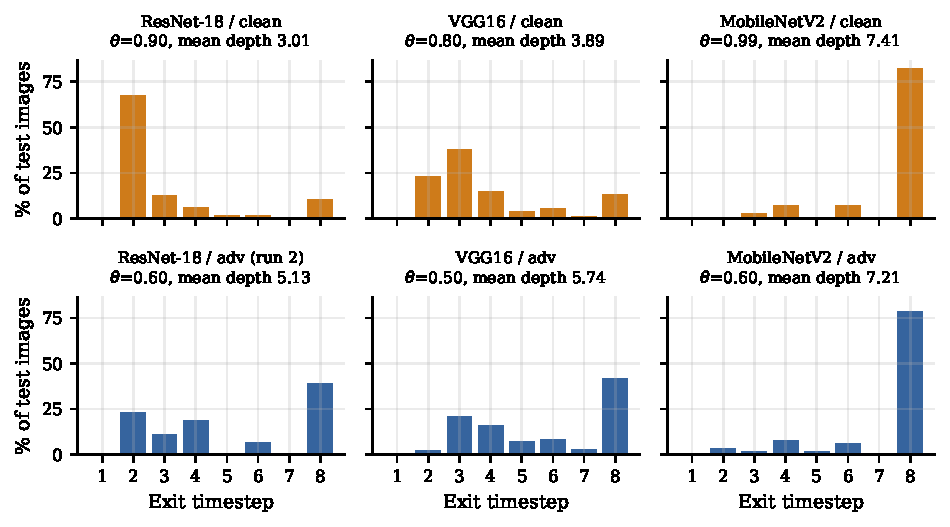
\includegraphics[width=\textwidth]{exit_histograms}
    \caption[Distribution of exit timesteps at the VT-neutral operating points]{Distribution of exit timesteps at the VT-neutral operating points (test set). Clean-trained models (top) concentrate exits early, while adversarially trained models (bottom) send a large fraction of inputs to the full horizon.}
    \label{fig:exit-hist}
\end{figure}

For the clean-trained ResNet-18, 67\% of test images exit at $t = 2$, the earliest step at which a fixed-T8 model has any information, and only 10\% run to $t = 8$. The VT gain comes from this bimodality: most images are already classified correctly and confidently at $t = 2$, and the compute saved on them is spent on the minority that need the full horizon. A fixed horizon of $T = 3$ spends the same total compute uniformly and so under-serves the hard images. VGG16 shows the same pattern with exits centred one step later, consistent with its slower fixed-timestep saturation.

Adversarially trained models are less confident: 39--42\% of test images run to $t = 8$ on ResNet-18 and VGG16, and their softmax confidence rarely exceeds high thresholds, which is why their VT-neutral thresholds are low (0.5--0.6). MobileNetV2 sends about 80\% of images to the full horizon in both regimes, leaving little room for savings. Exits at $t = 1$ never occur for fixed-T8 models (their $t = 1$ output is uninformative) but account for 7--8\% of exits for mixed-T models.

\subsection{Effect of the training schedule}
\label{sec:res-mixt}

\figref{fig:mixt} compares the fixed-T8 and mixed-T ResNet-18 frontiers. Under adversarial training, mixed-T training raises the fixed-timestep curve at every horizon, and most at short horizons, which is exactly where VT drew its advantage. Under clean training, the fixed-timestep curve barely moves in accuracy but shifts to the right in compute, because the mixed-T network is less sparse. The VT curve, however, moves down: at $\theta = 0.95$ the mixed-T VT model reaches 84.15\% at $2.02 \times 10^{8}$ SynOps, below the fixed horizon $T = 3$ (86.75\% at $1.91 \times 10^{8}$).

\begin{figure}[htbp]
    \centering
    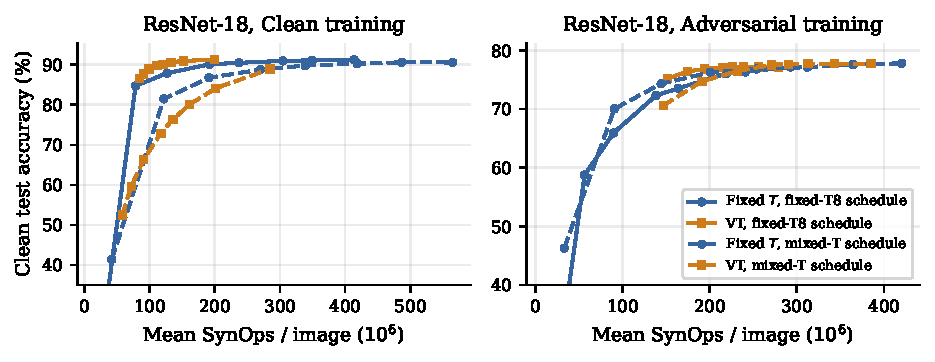
\includegraphics[width=\textwidth]{mixT_frontiers}
    \caption[Effect of the training schedule on the ResNet-18 frontiers]{Effect of the training schedule on the ResNet-18 frontiers (test set). Solid lines show the fixed-T8 schedule and dashed lines the mixed-T schedule.}
    \label{fig:mixt}
\end{figure}

The gain of VT shrinks under mixed-T training: from $+2.73$ to $+0.14$ for clean training and from $+2.89$ (run 2, or $+1.37$ for run 1) to $+0.68$ for adversarial training, and only 3 and 5 of the 8 thresholds lie above the frontier. For the clean mixed-T model, no threshold came within $\delta = 1$ point of the full horizon on the calibration split, so the most accurate threshold ($\theta = 0.99$) was used, 1.65 points below full.

The two regimes therefore lose the VT advantage for different reasons. Under adversarial training, the baseline gets stronger: a model trained across horizons is a much better short-horizon classifier, and per-input stopping adds little to it. Under clean training, the stopping signal gets worse: the mixed-T model is trained to commit to a prediction after one or two timesteps, and 43\% of test images exit at $t \le 2$ even at $\theta = 0.99$ (\figref{fig:exit-hist} shows the fixed-T8 models for contrast), but its early confidence is a poorer indicator of correctness than that of the fixed-T8 model. In both cases, VT's advantage is largest when the fixed-horizon model has not been trained for short horizons but still produces confident and correct early predictions on easy inputs. This also means that VT's efficiency gain should be compared not only with a compute-matched horizon but with a \emph{training-matched} one: a fair baseline for VT is a fixed-horizon model trained for the horizon at which it will be run. Mixed-T training is not free, however: on clean data it makes the network less sparse, and its VT points require more SynOps for the same accuracy than the fixed-T8 model's VT points do (\figref{fig:mixt}, left).

\section{Stopping Rules}
\label{sec:res-stoprules}

Does the conclusion depend on using the maximum softmax probability as the confidence score? \tabref{tab:res-stoprules} and \figref{fig:stoprules} compare the five stopping rules at approximately equal mean depth on the configurations where the reference depth is meaningful. (For the clean mixed-T ResNet-18 and the clean MobileNetV2, the stopping-rule comparison was calibrated to the depth of the degenerate max-gain operating point discussed in \secref{sec:res-selection}, so their rows are relegated to Appendix~\ref{app:tables}.)

\begin{table}[htbp]
    \centering
    \caption[Stopping-rule comparison]{Stopping-rule comparison (test accuracy \% at mean exit depth in parentheses). Each rule's threshold was calibrated to match the depth of the max-softmax operating point.}
    \label{tab:res-stoprules}
    \footnotesize
    \setlength{\tabcolsep}{3pt}
    \begin{tabular}{@{}l c c c c c c@{}}
        \toprule
        Configuration & Fixed $T{=}8$ & Max softmax & Margin & Entropy & Temp.\ softmax & Evidential \\
        \midrule
        R18 clean    & 91.26 & 88.91 (2.39) & 89.04 (2.38) & 88.14 (2.34) & 89.35 (2.59) & 86.38 (2.19) \\
        R18 adv (1)  & 73.67 & 71.48 (4.33) & 73.31 (5.42) & 72.24 (5.00) & 73.61 (6.16) & 67.99 (3.75) \\
        R18 adv (2)  & 77.18 & 76.42 (5.13) & 76.77 (5.46) & 76.04 (5.19) & 77.14 (6.25) & 73.16 (4.62) \\
        R18 adv mixT & 77.79 & 77.50 (5.43) & 77.47 (5.50) & 77.41 (5.42) & 77.37 (5.43) & 76.13 (6.04) \\
        VGG clean    & 88.20 & 86.99 (3.53) & 86.99 (3.50) & 86.11 (3.44) & 87.39 (3.82) & 82.54 (2.95) \\
        VGG adv      & 65.52 & 65.21 (6.27) & 65.40 (6.63) & 64.46 (6.17) & 65.45 (7.02) & 62.22 (5.22) \\
        MBv2 adv     & 51.44 & 50.92 (7.21) & 51.30 (7.49) & 50.91 (7.35) & 51.49 (7.89) & 49.48 (6.61) \\
        \bottomrule
    \end{tabular}
\end{table}

\begin{figure}[htbp]
    \centering
    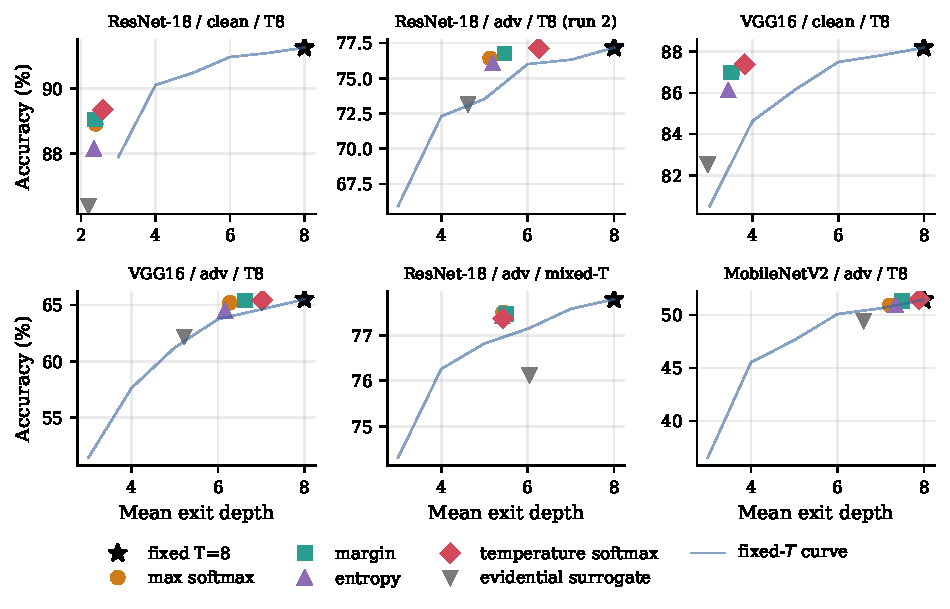
\includegraphics[width=\textwidth]{stopping_rules}
    \caption[Stopping rules compared at matched exit depth]{Stopping rules compared at matched exit depth. The thin line is the fixed-timestep curve, and points above it are better than a fixed horizon of the same depth.}
    \label{fig:stoprules}
\end{figure}

Three findings emerge. First, \textbf{all four softmax-based rules lie above the fixed-timestep curve} on every configuration in \figref{fig:stoprules}: the VT advantage is not specific to the max-softmax score. Second, max softmax, margin and entropy are within about one point of each other wherever they land at the same depth. Differences that look larger (for example 71.48\% vs 73.31\% on R18 adv (1)) come with a full timestep of extra depth, because the depth calibration on a discrete threshold grid is coarse. Temperature softmax tends to land deeper and correspondingly more accurately. Third, \textbf{the evidential surrogate is consistently the worst}: it is 1.4--4.5 points less accurate than max softmax, usually while exiting earlier, and lands on or only slightly above the fixed-timestep curve. On R18 adv mixT it lands deeper (6.04) yet less accurate, below the fixed curve. Its uncertainty mass saturates quickly for large logits, so it exits confidently on inputs that are not yet correctly classified. The choice among the softmax-based rules is therefore a second-order concern, and we use max softmax throughout.

\section{RQ4: Sensitivity to the Selection Rule}
\label{sec:res-selection}

\subsection{Max-gain selection is biased}

\tabref{tab:res-selection} compares the operating points chosen by the max-gain rule (used in our original experiments) with the VT-neutral points of \tabref{tab:res-neutral}, and \figref{fig:selection} visualises the difference.

\begin{table}[htbp]
    \centering
    \caption[Max-gain versus VT-neutral operating points]{Max-gain versus VT-neutral ($\delta = 1$) operating points (test set). Max-gain selection chooses the threshold with the largest calibration gain over its matched control.}
    \label{tab:res-selection}
    \small
    \setlength{\tabcolsep}{4pt}
    \begin{tabular}{@{}l c c r r r @{\hspace{12pt}} c c r r@{}}
        \toprule
        & \multicolumn{5}{c}{Max-gain selection} & \multicolumn{4}{c}{VT-neutral selection} \\
        \cmidrule(r{12pt}){2-6} \cmidrule(l){7-10}
        Configuration & $\theta$ & Depth & VT acc & Gain & Below full & $\theta$ & Depth & Gain & Below full \\
        \midrule
        R18 clean       & 0.70 & 2.39 & 88.91 & $+4.19$  & 2.35  & 0.90 & 3.01 & $+2.73$ & 0.64 \\
        R18 adv (1)     & 0.50 & 4.33 & 71.48 & $+2.13$  & 2.19  & 0.60 & 5.01 & $+1.37$ & 0.84 \\
        R18 adv (2)     & 0.60 & 5.13 & 76.42 & $+2.89$  & 0.76  & 0.60 & 5.13 & $+2.89$ & 0.76 \\
        R18 clean mixT  & 0.60 & 1.38 & 59.63 & $+18.24$ & 30.94 & 0.99 & 4.24 & $+0.14$ & 1.65 \\
        R18 adv mixT    & 0.80 & 5.43 & 77.50 & $+0.68$  & 0.29  & 0.80 & 5.43 & $+0.68$ & 0.29 \\
        VGG clean       & 0.70 & 3.53 & 86.99 & $+6.49$  & 1.21  & 0.80 & 3.89 & $+3.12$ & 0.45 \\
        VGG adv         & 0.60 & 6.27 & 65.21 & $+1.46$  & 0.31  & 0.50 & 5.74 & $+0.89$ & 0.88 \\
        MBv2 clean      & 0.50 & 2.38 & 28.96 & $+11.36$ & 48.70 & 0.99 & 7.41 & $+3.37$ & $-0.42$ \\
        MBv2 adv        & 0.60 & 7.21 & 50.92 & $+0.28$  & 0.52  & 0.60 & 7.21 & $+0.28$ & 0.52 \\
        \bottomrule
    \end{tabular}
\end{table}

\begin{figure}[htbp]
    \centering
    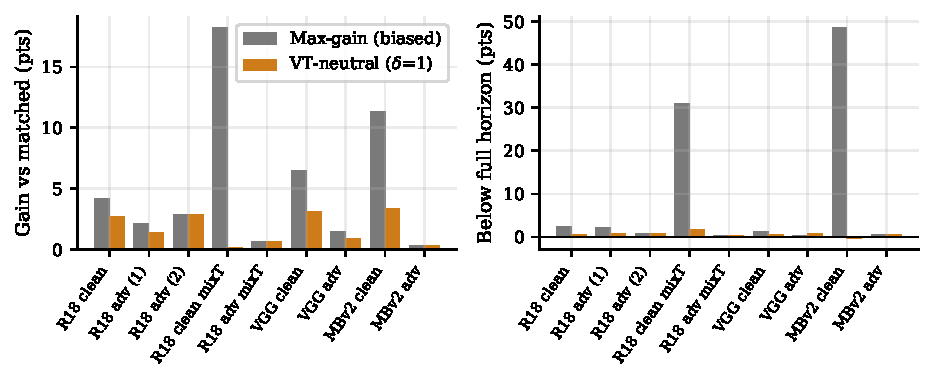
\includegraphics[width=\textwidth]{selection_bias}
    \caption[Effect of the selection rule on the reported gain]{Effect of the selection rule. Left: gain over the compute-matched control. Right: accuracy given up relative to the full horizon. Max-gain selection inflates the gain on six of nine configurations, and on two it selects operating points 31--49 points below the full horizon.}
    \label{fig:selection}
\end{figure}

On three configurations the two rules agree. On the other six, max-gain selection reports a larger gain, in five of them by choosing a lower threshold (earlier exits) than the VT-neutral rule. The inflation is moderate where both points are reasonable: $+4.19$ instead of $+2.73$ on R18 clean, $+6.49$ instead of $+3.12$ on VGG clean. On two configurations it is extreme. For the clean mixed-T ResNet-18, max-gain selection picks $\theta = 0.60$, where VT reaches only 59.63\% with a mean depth of 1.38, and reports an $+18.24$ point gain over $T = 1$ (41.39\%). For the clean MobileNetV2 it picks $\theta = 0.50$, where VT reaches 28.96\%, and reports an $+11.36$ point gain over $T = 2$ (17.60\%). Both operating points are useless in practice, at 31 and 49 points below the full-horizon accuracy, and the large gains are comparisons between two bad models, one slightly less bad than the other.

The mechanism is simple. Near the start of the fixed-timestep curve, accuracy rises steeply with compute, so VT's ability to spend slightly more compute on some inputs buys a large accuracy difference relative to the matched horizon. Maximising the gain therefore drives the selection towards the steepest part of the fixed curve, which is also where both models are least accurate. The rule rewards VT for the very comparison it is being evaluated on.

In our original experiments this failure was caught for MobileNetV2 by inspection and overridden by hand with $\theta = 0.95$, and the attack experiments for that configuration use this threshold. It was not caught for the mixed-T ResNet-18, whose attack experiments therefore use the degenerate $\theta = 0.60$. The VT-neutral rule removes the need for such judgement calls.

\subsection{Sensitivity to the tolerance}

The VT-neutral rule has one parameter, the tolerance $\delta$. \tabref{tab:res-delta} and \figref{fig:delta} report the gain at $\delta \in \{0.5, 1, 2\}$.

\begin{table}[htbp]
    \centering
    \caption{Gain over the compute-matched control (points) under VT-neutral selection with tolerance $\delta$.}
    \label{tab:res-delta}
    \small
    \begin{tabular}{@{}l r r r@{}}
        \toprule
        Configuration & $\delta = 0.5$ & $\delta = 1$ & $\delta = 2$ \\
        \midrule
        R18 clean       & $+1.15$ & $+2.73$ & $+2.24$ \\
        R18 adv (1)     & $+2.03$ & $+1.37$ & $+1.37$ \\
        R18 adv (2)     & $+2.89$ & $+2.89$ & $+1.62$ \\
        R18 clean mixT  & $+0.14$ & $+0.14$ & $+0.14$ \\
        R18 adv mixT    & $+0.68$ & $+0.68$ & $-0.35$ \\
        VGG clean       & $+3.31$ & $+3.12$ & $+6.49$ \\
        VGG adv         & $+1.46$ & $+0.89$ & $+0.89$ \\
        MBv2 clean      & $+3.37$ & $+3.37$ & $+3.37$ \\
        MBv2 adv        & $-0.06$ & $+0.28$ & $+0.28$ \\
        \bottomrule
    \end{tabular}
\end{table}

\begin{figure}[htbp]
    \centering
    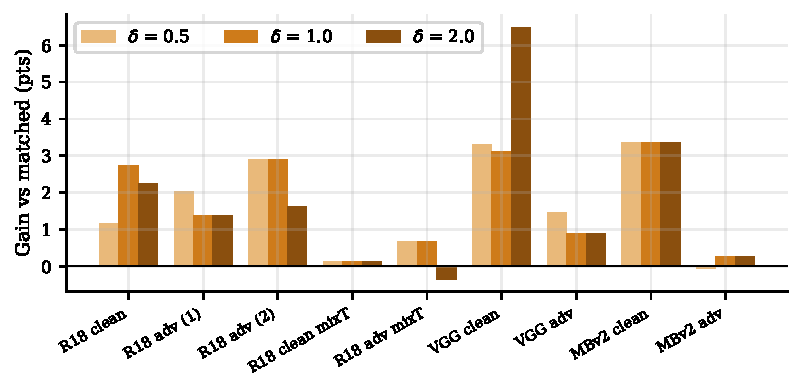
\includegraphics[width=\textwidth]{delta_sensitivity}
    \caption{Sensitivity of the VT-neutral gain to the tolerance $\delta$.}
    \label{fig:delta}
\end{figure}

The sign of the gain is stable: 25 of the 27 entries are positive, and the two negative entries ($-0.35$ and $-0.06$) are on the two configurations whose gains were already within noise. The magnitude is not stable: because the threshold grid is discrete and the fixed horizon is an integer, changing $\delta$ can move the selected threshold by one grid step and the matched horizon by one timestep, which can change the gain by one to three points (from $+1.15$ to $+2.73$ on R18 clean and from $+3.12$ to $+6.49$ on VGG clean). The qualitative conclusions of \secref{sec:res-efficiency} hold for every $\delta$: clear gains on clean fixed-T8 ResNet-18 and VGG16, smaller gains under adversarial training and negligible gains under mixed-T training. However, but single-point gain values should be read with roughly $\pm 1.5$ points of selection uncertainty in addition to evaluation noise.

\section{RQ2: Adversarial Robustness}
\label{sec:res-robustness}

We now ask how VT changes robustness. This section reports the single-run results for every configuration, and \secref{sec:res-multiseed} then tests which of them replicate. All attacks are white-box with $\epsilon = 8/255$, and the attacker differentiates through the exit-step logits of the VT model (\secref{sec:meth-attacks}). As explained in \secref{sec:meth-selection}, the attacked VT thresholds are those chosen by the original max-gain rule (with the MobileNetV2 override to $\theta = 0.95$). For the adversarially trained models these coincide with or neighbour the VT-neutral thresholds.

\subsection{Clean-trained models have no robustness to lose}

\tabref{tab:res-robust} shows that every clean-trained model collapses under attack, with or without VT. ResNet-18 and VGG16 are at or near 0\% under both PGD-20 and AutoAttack, and MobileNetV2 retains about 5\%. The differences between fixed and VT inference are a fraction of a point (the 2.25\% of the clean mixed-T ResNet-18 under AutoAttack is at its degenerate $\theta = 0.60$ point, where clean accuracy is only 59.63\%). Without adversarial training, VT neither helps nor hurts robustness, because there is no robustness to help or hurt. The rest of this section concerns adversarially trained models.

\begin{table}[htbp]
    \centering
    \caption[Single-run robustness of fixed and VT inference]{Single-run robust accuracy (\%) of full-horizon ($T=8$) and VT inference under PGD-20 and AutoAttack ($\epsilon = 8/255$). $\theta$: attacked threshold. $n$: number of attacked images. The run-1 adversarial ResNet-18 is omitted (see \secref{sec:res-threats}).}
    \label{tab:res-robust}
    \small
    \setlength{\tabcolsep}{4pt}
    \begin{tabular}{@{}l c r r r r r r r@{}}
        \toprule
        & & & \multicolumn{3}{c}{PGD-20} & \multicolumn{3}{c}{AutoAttack} \\
        \cmidrule(lr){4-6} \cmidrule(l){7-9}
        Configuration & $\theta$ & $n$ & $T{=}8$ & VT & $\Delta$ & $T{=}8$ & VT & $\Delta$ \\
        \midrule
        R18 clean       & 0.70 & 10{,}000 & 0.00 & 0.02 & $+0.02$ & 0.06 & 0.02 & $-0.04$ \\
        R18 clean mixT  & 0.60 & 2{,}000  & 0.00 & 0.15 & $+0.15$ & 0.10 & 2.25 & $+2.15$ \\
        VGG clean       & 0.70 & 2{,}000  & 0.05 & 0.10 & $+0.05$ & 0.00 & 0.00 & $+0.00$ \\
        MBv2 clean      & 0.95 & 2{,}000  & 5.10 & 4.95 & $-0.15$ & 5.25 & 5.40 & $+0.15$ \\
        \midrule
        R18 adv (2)     & 0.60 & 2{,}000  & 46.10 & 48.70 & $+2.60$ & 28.85 & 24.15 & $-4.70$ \\
        R18 adv mixT    & 0.80 & 2{,}000  & 40.85 & 41.50 & $+0.65$ & 29.45 & 25.55 & $-3.90$ \\
        VGG adv         & 0.60 & 2{,}000  & 45.90 & 44.45 & $-1.45$ & 10.75 & 8.55  & $-2.20$ \\
        MBv2 adv        & 0.60 & 2{,}000  & 35.60 & 34.75 & $-0.85$ & 27.60 & 27.55 & $-0.05$ \\
        \bottomrule
    \end{tabular}
\end{table}

\subsection{PGD and AutoAttack disagree}

For the adversarially trained models, the two attacks tell different stories (\figref{fig:pgd-aa}). Under PGD-20, VT is within $\pm 2.6$ points of the full-horizon model and is \emph{better} on two of four configurations. A reader who saw only PGD would conclude that VT costs nothing in robustness. Under AutoAttack, VT is worse than the full horizon on every adversarially trained configuration, by up to 4.7 points (and tied, at $-0.05$, on MobileNetV2, whose VT point runs 7.2 of 8 timesteps).

\begin{figure}[htbp]
    \centering
    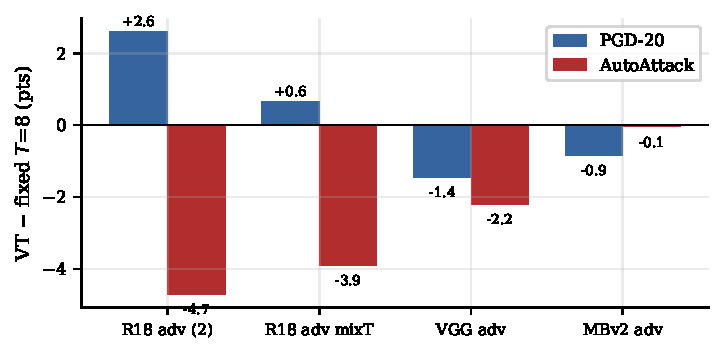
\includegraphics[width=0.85\textwidth]{pgd_aa_gap}
    \caption[VT versus the full horizon under PGD-20 and AutoAttack]{Robust accuracy of VT minus that of the full-horizon model ($T = 8$), single run, adversarially trained models. PGD-20 suggests that VT is as robust as the full horizon, but AutoAttack shows that it is less robust.}
    \label{fig:pgd-aa}
\end{figure}

The gap between PGD and AutoAttack is itself large: 11--17 points for ResNet-18, 8 points for MobileNetV2 and 35 points for VGG16 at the full horizon. Gaps of this size indicate that PGD-20 is far from the worst case for these models. For VGG16 in particular, its PGD robustness is largely illusory. This matches the conclusion of Wang et al.~\cite{wang2026towards} that SNN robustness is often over-estimated by standard gradient attacks, and it means that \emph{any} statement about VT and robustness made on the basis of PGD alone should be treated with suspicion. The direction of VT's effect also differs between the attacks: the gradient-free Square attack and the adaptive-step APGD in AutoAttack are evidently able to exploit something that PGD misses, and the multi-seed experiments below locate what it is.

\subsection{What attacks do to exit depth}
\label{sec:res-probe}

Attacks change not only VT's predictions but also when it stops. On adversarially trained models, untargeted PGD \emph{increases} the mean exit depth: from 5.13 to 5.86 timesteps on R18 adv (2), from 6.27 to 6.69 on VGG adv, from 7.21 to 7.45 on MBv2 adv and from 5.43 to 6.35 on R18 adv mixT. On clean-trained models it does the opposite: the attacked inputs of R18 clean exit at a mean depth of 2.00 (from 2.39 on clean inputs) and those of VGG clean at 2.40 (from 3.53). The adversary makes clean-trained models confidently wrong at the first informative timestep, while adversarially trained models become less confident and keep integrating.

\figref{fig:probe} shows why for an adversarially trained ResNet-18 (1{,}000 test images). Under PGD-20 the running prediction is less accurate at every timestep, and its mean confidence is lower: at $t = 8$ the mean max-softmax confidence is 0.61 on attacked inputs against 0.68 on clean ones, so attacked inputs cross a threshold of 0.60 later. Robust accuracy rises from 36\% at $t = 2$ to 49\% at $t = 8$, a 12.5-point gain from integrating six more timesteps, proportionally as large as the corresponding clean gain (from 57\% to 78\%). This is the central mechanism behind the robustness results: \textbf{for an adversarially trained SNN, robustness accumulates over timesteps}. An inference mode that runs fewer timesteps has, on average, less of it.

\begin{figure}[htbp]
    \centering
    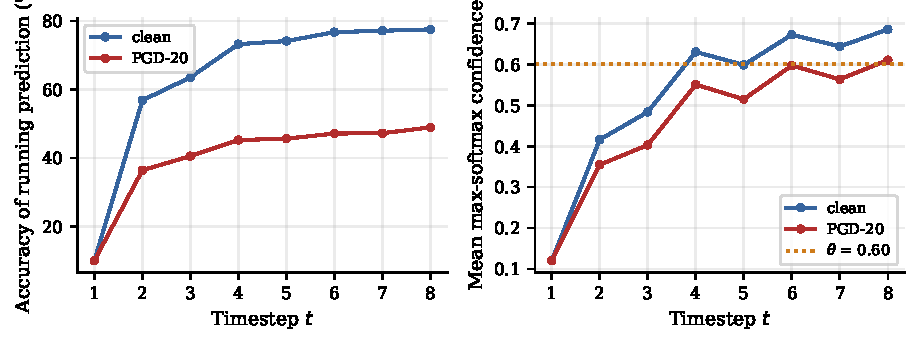
\includegraphics[width=\textwidth]{probe_trajectory}
    \caption[Accuracy and confidence of the running prediction over timesteps]{Accuracy (left) and mean max-softmax confidence (right) of the running prediction at each timestep for an adversarially trained fixed-T8 ResNet-18, on clean and PGD-20 inputs (1{,}000 test images). Robust accuracy keeps rising with the number of timesteps, and attacked inputs are less confident and cross the threshold later.}
    \label{fig:probe}
\end{figure}

\section{RQ3: The Exit Gate as an Attack Surface}
\label{sec:res-gate}

\subsection{Wrong early exit}

The wrong-early-exit attack (\eqnref{eq:wrong-exit}) explicitly tries to make inputs exit early with a wrong label. \tabref{tab:res-wrong-exit} compares it with untargeted PGD on the same VT operating points.

\begin{table}[htbp]
    \centering
    \caption[Wrong-early-exit attack versus untargeted PGD]{Wrong-early-exit attack versus untargeted PGD-20 at the attacked VT threshold (robust accuracy \%, with mean exit depth in parentheses). $n = 2{,}000$ except for R18 clean ($n = 10{,}000$).}
    \label{tab:res-wrong-exit}
    \small
    \begin{tabular}{@{}l c c c r@{}}
        \toprule
        Configuration & $\theta$ & Untargeted PGD-20 & Wrong early exit & $\Delta$ acc \\
        \midrule
        R18 clean      & 0.70 & 0.02 (2.00) & 0.00 (2.00) & $-0.02$ \\
        R18 clean mixT & 0.60 & 0.15 (1.02) & 2.60 (1.18) & $+2.45$ \\
        VGG clean      & 0.70 & 0.10 (2.40) & 0.00 (2.45) & $-0.10$ \\
        MBv2 clean     & 0.95 & 4.95 (7.17) & 4.05 (6.95) & $-0.90$ \\
        \midrule
        R18 adv (2)    & 0.60 & 48.70 (5.86) & 45.95 (5.62) & $-2.75$ \\
        R18 adv mixT   & 0.80 & 41.50 (6.35) & 42.55 (6.27) & $+1.05$ \\
        VGG adv        & 0.60 & 44.45 (6.69) & 46.35 (6.62) & $+1.90$ \\
        MBv2 adv       & 0.60 & 34.75 (7.45) & 33.35 (7.42) & $-1.40$ \\
        \bottomrule
    \end{tabular}
\end{table}

The gate-aware objective is not a stronger misclassification attack than ordinary PGD. On clean-trained models both attacks reach about 0\%, and untargeted PGD \emph{already} produces wrong early exits: attacked inputs leave at the earliest informative timestep. On adversarially trained models the two attacks are within $\pm 3$ points of each other (comparable to the $\pm 2$ point evaluation noise) and neither consistently wins. The wrong-early-exit attack shortens the mean depth by at most a quarter of a timestep. The adversarially trained models' low confidence under attack (\figref{fig:probe}) makes it hard for any attack to force a confident early exit within the $\epsilon$ budget. We conclude that, within our threat model, the exit gate does not open a new route to misclassification beyond what standard attacks already find.

\subsection{Compute overuse}

The compute-overuse attack (\eqnref{eq:overuse}) has the opposite goal: keep the prediction correct but delay the exit. \tabref{tab:res-overuse} and \figref{fig:overuse} report the inflation of mean exit depth it achieves.

\begin{table}[htbp]
    \centering
    \caption[Compute-overuse attack]{Compute-overuse attack at the attacked VT threshold. Clean depth: mean exit depth on clean test inputs. Inflation: increase in mean exit depth under attack. Headroom: inflation as a fraction of the timesteps available, $8 - \text{clean depth}$. Kept: accuracy on attacked inputs (the attack aims to preserve the label).}
    \label{tab:res-overuse}
    \small
    \begin{tabular}{@{}l c c c r r r@{}}
        \toprule
        Configuration & $\theta$ & Clean depth & Attacked depth & Inflation & Headroom & Kept (\%) \\
        \midrule
        R18 clean       & 0.70 & 2.39 & 3.58 & $+1.19$ & 21\% & 60.6 \\
        R18 clean mixT  & 0.60 & 1.38 & 1.55 & $+0.17$ & 3\%  & 81.6 \\
        VGG clean       & 0.70 & 3.53 & 4.70 & $+1.17$ & 26\% & 72.1 \\
        MBv2 clean      & 0.95 & 6.56 & 7.71 & $+1.15$ & 80\% & 97.2 \\
        \midrule
        R18 adv (1)     & 0.50 & 4.33 & 4.70 & $+0.37$ & 10\% & 86.5 \\
        R18 adv (2)     & 0.60 & 5.13 & 5.40 & $+0.27$ & 10\% & 92.0 \\
        R18 adv mixT    & 0.80 & 5.43 & 6.08 & $+0.65$ & 25\% & 95.0 \\
        VGG adv         & 0.60 & 6.27 & 6.31 & $+0.04$ & 2\%  & 81.0 \\
        MBv2 adv        & 0.60 & 7.21 & 7.26 & $+0.05$ & 7\%  & 67.1 \\
        \bottomrule
    \end{tabular}
\end{table}

\begin{figure}[htbp]
    \centering
    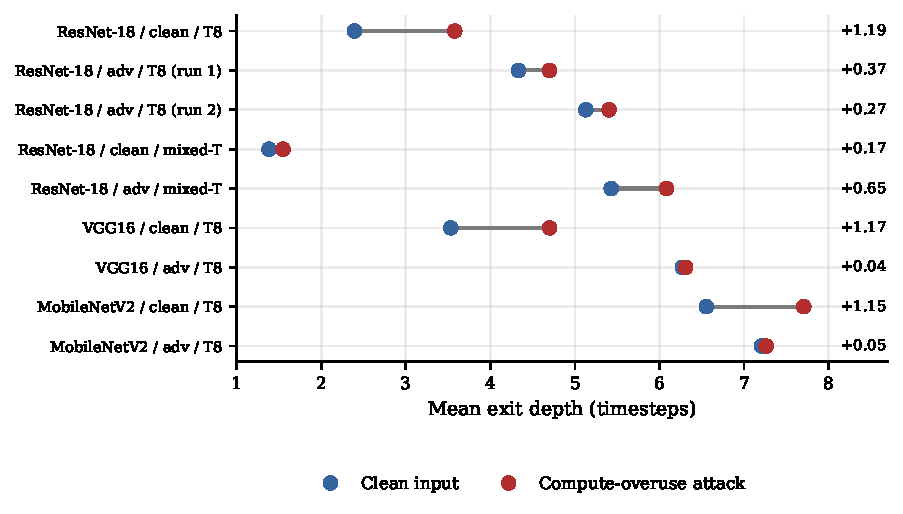
\includegraphics[width=0.85\textwidth]{compute_overuse}
    \caption[Exit-depth inflation under the compute-overuse attack]{Mean exit depth on clean inputs (blue) and under the label-preserving compute-overuse attack (red) at the attacked VT threshold. Numbers on the right give the inflation in timesteps.}
    \label{fig:overuse}
\end{figure}

\paragraph{Clean-trained fixed-T8 models are highly vulnerable.} On all three backbones, the attack raises the mean exit depth of the clean-trained fixed-T8 model by more than one full timestep (1.15--1.19), using 21--80\% of the available headroom. For the clean ResNet-18 this means a 50\% increase in exit depth (2.39 to 3.58 timesteps), eroding a substantial part of the compute saving that motivated VT. The attack preserves the label on 61--97\% of inputs. A perturbation that is invisible to accuracy monitoring yet substantially increases energy consumption is precisely the threat that motivates sponge and slowdown attacks~\cite{shumailov2021sponge, hong2021panda}, and VT SNNs are susceptible to it.

\paragraph{Adversarial training largely removes the vulnerability.} On adversarially trained fixed-T8 models, inflation falls to 0.04--0.37 timesteps (2--10\% of headroom). This is not only a ceiling effect from their higher clean depth: as a fraction of available headroom the inflation is two (ResNet-18) to more than ten (VGG16, MobileNetV2) times smaller than for clean-trained models. Adversarial training flattens the network's confidence response to small input perturbations in general, and that protects the exit gate as a side effect. The exception is the adversarially trained mixed-T ResNet-18, whose inflation (0.65 timesteps, 25\% of headroom) is comparable to that of clean-trained models. The mixed-T schedule, which trains the network to commit at short horizons, seems to make its early confidence more malleable.

\paragraph{Clean mixed-T.} The low inflation of the clean mixed-T ResNet-18 (0.17) is an artefact of its degenerate attacked threshold ($\theta = 0.60$, depth 1.38), at which most inputs exit at $t \le 2$ regardless, so it should not be read as robustness.

\subsection{Summary of the attack surface}

The exit gate creates one new practical vulnerability and not the one usually feared. It does not make misclassification easier, but it makes \emph{compute} attackable: a VT model's energy cost becomes a function of the input that an adversary can raise while leaving accuracy intact. The vulnerability is severe for clean-trained models and largely mitigated by adversarial training. A deployment that relies on VT for an energy or latency budget should therefore either use adversarially trained models or enforce a hard compute cap.

\section{Multi-Seed Replication}
\label{sec:res-multiseed}

The single-run results contain both effects that may be real and effects that may be noise. The two identical ResNet-18 adversarial runs differ by 3.5 points of full-horizon accuracy and by a factor of two in VT gain (\tabref{tab:res-neutral}), so single runs cannot settle which is which. This section reports the three-seed replication for adversarially trained ResNet-18 and VGG16.

\subsection{Per-seed results}

\tabref{tab:res-multiseed} lists the results for each of the six checkpoints. All three inference modes are evaluated on the same 1{,}000 class-balanced test images.

\begin{table}[htbp]
    \centering
    \caption[Multi-seed results per checkpoint]{Multi-seed results per checkpoint (accuracy \%, $n = 1{,}000$). Full: $T = 8$. Matched: compute-matched fixed horizon ($T^* = 5$ for ResNet-18, $T^* = 6$ for VGG16). VT: selected threshold.}
    \label{tab:res-multiseed}
    \small
    \setlength{\tabcolsep}{4pt}
    \begin{tabular}{@{}l c c r r r r r r r r r@{}}
        \toprule
        & & & \multicolumn{3}{c}{Clean} & \multicolumn{3}{c}{PGD-20} & \multicolumn{3}{c}{AutoAttack} \\
        \cmidrule(lr){4-6} \cmidrule(lr){7-9} \cmidrule(l){10-12}
        Backbone & Seed & $\theta$ & Full & Match & VT & Full & Match & VT & Full & Match & VT \\
        \midrule
        \multirow{3}{*}{ResNet-18} & 0 & 0.5 & 78.6 & 74.7 & 76.0 & 56.3 & 56.4 & 57.0 & 32.0 & 23.4 & 24.3 \\
                                   & 1 & 0.5 & 77.8 & 72.8 & 74.9 & 50.7 & 49.2 & 51.0 & 31.7 & 24.6 & 29.9 \\
                                   & 2 & 0.6 & 74.7 & 72.3 & 75.3 & 47.3 & 48.9 & 48.3 & 24.8 & 20.2 & 22.2 \\
        \midrule
        \multirow{3}{*}{VGG16}     & 0 & 0.7 & 66.9 & 64.4 & 68.5 & 43.9 & 43.6 & 44.6 & 18.3 & 19.9 & 16.4 \\
                                   & 1 & 0.5 & 66.9 & 64.3 & 66.1 & 46.0 & 47.2 & 45.6 & 23.1 & 21.4 & 15.3 \\
                                   & 2 & 0.6 & 67.2 & 64.3 & 66.8 & 47.5 & 46.0 & 46.2 & 20.5 & 14.5 & 18.0 \\
        \bottomrule
    \end{tabular}
\end{table}

The checkpoints vary widely. Full-horizon AutoAttack accuracy ranges from 24.8\% to 32.0\% across ResNet-18 seeds and from 18.3\% to 23.1\% across VGG16 seeds, and seed 2 of ResNet-18 is about 3 points less accurate on clean data than seeds 0 and 1. Differences of this size between checkpoints are larger than most of the single-run effects in \secref{sec:res-robustness}, which is why the analysis below is based on paired, within-checkpoint differences.

\subsection{Paired tests}

\tabref{tab:res-pooled} reports the paired differences pooled over the six checkpoints, and \figref{fig:multiseed} shows every checkpoint's difference.

\begin{table}[htbp]
    \centering
    \caption[Pooled paired differences across six adversarially trained checkpoints]{Paired differences (VT minus reference, points) pooled over six adversarially trained checkpoints (three ResNet-18, three VGG16). $+$/$n$: checkpoints with a positive difference. $p_t$: one-sample $t$-test, 5 degrees of freedom. $p_{\mathrm{sign}}$: exact two-sided sign test.}
    \label{tab:res-pooled}
    \small
    \begin{tabular}{@{}l l r c r r r@{}}
        \toprule
        Reference & Metric & Mean $\pm$ SD & $+$/$n$ & $t$ & $p_t$ & $p_{\mathrm{sign}}$ \\
        \midrule
        \multirow{3}{*}{Matched fixed $T^*$} & Clean      & $+2.47 \pm 0.99$ & 6/6 & 6.11  & \textbf{0.002} & \textbf{0.031} \\
                                             & PGD-20     & $+0.23 \pm 1.20$ & 4/6 & 0.48  & 0.655 & 0.688 \\
                                             & AutoAttack & $+0.35 \pm 4.33$ & 4/6 & 0.20  & 0.851 & 0.688 \\
        \midrule
        \multirow{3}{*}{Full horizon $T=8$}  & Clean      & $-0.75 \pm 1.76$ & 2/6 & $-1.04$ & 0.345 & 0.688 \\
                                             & PGD-20     & $+0.17 \pm 0.87$ & 4/6 & 0.47  & 0.657 & 0.688 \\
                                             & AutoAttack & $-4.05 \pm 2.88$ & 0/6 & $-3.44$ & \textbf{0.018} & \textbf{0.031} \\
        \bottomrule
    \end{tabular}
\end{table}

\begin{figure}[htbp]
    \centering
    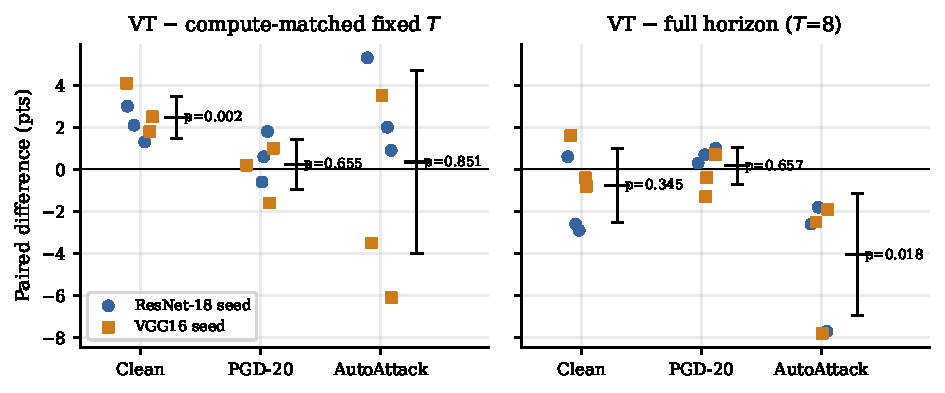
\includegraphics[width=\textwidth]{multiseed_paired}
    \caption[Paired multi-seed differences]{Paired differences for each adversarially trained checkpoint. Left: VT minus the compute-matched fixed horizon. Right: VT minus the full horizon. Black bars: mean $\pm$ one standard deviation, with the $t$-test $p$-value.}
    \label{fig:multiseed}
\end{figure}

Two results replicate on every checkpoint.

\paragraph{VT's clean efficiency gain replicates.} VT is more accurate than its compute-matched control on clean data on all six checkpoints, by $+2.47 \pm 0.99$ points ($t(5) = 6.11$, $p = 0.002$). The effect holds on each backbone separately ($+2.13 \pm 0.85$ for ResNet-18, $+2.80 \pm 1.18$ for VGG16). On clean data, VT is statistically indistinguishable from the full horizon ($-0.75$, $p = 0.35$) while running 18--39\% fewer timesteps on average. This answers RQ1 for adversarially trained models: the single-run gains of \tabref{tab:res-neutral} were not noise.

\paragraph{VT's AutoAttack cost relative to the full horizon replicates.} Under AutoAttack, VT is less robust than the full-horizon model on all six checkpoints, by $-4.05 \pm 2.88$ points ($t(5) = -3.44$, $p = 0.018$, sign test $p = 0.031$). The cost is the same on both backbones ($-4.03$ for ResNet-18, $-4.07$ for VGG16).

The comparisons that do not replicate are equally informative.

\paragraph{At equal compute, VT is as robust as a fixed horizon.} Against its matched control, VT's robustness difference is $+0.23 \pm 1.20$ under PGD-20 and $+0.35 \pm 4.33$ under AutoAttack, with four of six checkpoints positive in each case. There is no evidence that VT is more \emph{or} less robust than a fixed-horizon SNN that uses the same compute. The large AutoAttack variance is driven by VGG16, whose matched-control robustness varies between 14.5\% and 21.4\% across seeds.

\paragraph{PGD hides the cost.} Under PGD-20, VT is indistinguishable from the full horizon ($+0.17 \pm 0.87$), and on ResNet-18 it is even slightly better on all three seeds. The AutoAttack deficit of 4 points is invisible to PGD.

\subsection{Interpretation: robustness follows compute}

Taken together, the multi-seed results say that \emph{VT's robustness cost is a compute cost}. VT runs adversarially trained models for about five (ResNet-18) to six and a half (VGG16) timesteps on average instead of eight, and under AutoAttack it loses about four points relative to the full horizon. The compute-matched fixed horizon, which runs the same number of timesteps for every input, loses a similar amount: its AutoAttack accuracy is on average 4.4 points below the full horizon on the same checkpoints (\tabref{tab:res-multiseed}). VT and the matched horizon are, within the precision of our experiment, equally robust. What VT gives up is the robustness that the skipped timesteps would have provided, which is exactly what the confidence trajectories of \figref{fig:probe} predict: for adversarially trained SNNs, robust accuracy keeps rising with the number of timesteps integrated.

This interpretation reconciles the efficiency and robustness results. VT is a better way to spend a given compute budget on clean data, because it allocates timesteps to the inputs that need them. Under a strong attack, every input is hard, the confidence of attacked inputs is low, and the advantage of adaptive allocation disappears. What remains is the total compute spent, and VT spends less of it than the full horizon.

\subsection{Attack-seed variance}

To verify that the attack itself is not a significant source of variance, PGD-20 and AutoAttack were repeated with three attack seeds on one checkpoint per backbone. \tabref{tab:app-attack-seed} in Appendix~\ref{app:tables} lists the results. The standard deviation across attack seeds is at most 1.74 points and usually below one point, much smaller than the variance across training seeds. The conclusions above are therefore limited by training variance, not by attack randomness.

\section{Discussion}
\label{sec:res-discussion}

\subsection{What VT is, and what it is not}

The results support a precise statement of what variable timing does. On clean data, VT is a genuinely better allocation of compute than truncating every input at the same horizon: at equal measured SynOps it is 1--3 points more accurate on the configurations where there is something to save, it can reach within a point of the full horizon at 35--68\% lower compute, and the advantage replicates across seeds. Its benefit is largest for networks trained at the full horizon only and shrinks for networks trained across horizons, so part of what VT exploits is the poor short-horizon performance of fixed-T8-trained networks.

VT is \emph{not} a robustness mechanism, positively or negatively, at equal compute. Our data do not support the hypothesis that adaptive exit makes SNNs more fragile, nor the hypothesis that it makes them more robust. They support a simpler one: robustness of adversarially trained SNNs grows with the number of timesteps integrated, and VT integrates fewer.

\subsection{Why PGD-only evaluation would have misled us}

Had we evaluated only with PGD-20, we would have concluded that VT saves 40\% of compute at no cost in robustness, which is a strong and false claim. Two properties of the setting conspire to produce this. First, the PGD--AutoAttack gap is large for SNNs (8--35 points at the full horizon in our models), so PGD robustness numbers are far from the worst case. Second, VT's robustness cost is smaller than that gap, so it is hidden inside it. Any evaluation of an efficiency method for SNNs that reports robustness should use AutoAttack or an equally strong adaptive attack, compare with a compute-matched baseline, and replicate across seeds.

\subsection{Compute as an attack surface}

The compute-overuse results suggest that energy should be treated as a security property of VT SNNs. A clean-trained VT model that is deployed because it saves 60--70\% of compute can be made to run roughly 50\% more timesteps by an imperceptible perturbation, without any change in its accuracy. Adversarial training reduces this to a few percent of the headroom, but at a 14--26 point cost in clean accuracy. A practical middle ground would be to cap the compute any single input may use, or to monitor the distribution of exit depths at run time for signs of manipulation.

\subsection{Recommendations for evaluating VT}

From these results we draw five recommendations for future evaluations of variable timing and similar early-exit methods in SNNs:

\begin{enumerate}
    \item Compare every VT operating point with the fixed horizon of \emph{equal measured compute}, using sample-exact accounting, not only with the full horizon.
    \item Select operating points with a rule that does not reward the comparison being made (for example, the VT-neutral rule), on a split separate from the test set, and report depth and saving alongside every gain.
    \item Compare against a fixed-horizon model that was trained for short horizons (for example with a mixed-T schedule), not only one trained at the full horizon.
    \item Evaluate robustness with AutoAttack or an equally strong adaptive attack, with gradients taken through the deployed exit rule, and report the compute-matched and full-horizon comparisons separately.
    \item Report compute under attack, including a dedicated compute-overuse attack, and replicate key comparisons across training seeds with paired tests.
\end{enumerate}

\section{Threats to Validity}
\label{sec:res-threats}

\subsection{Internal validity}

\paragraph{Operating points for attacks.} The attack experiments were run at the thresholds chosen by the max-gain rule (\secref{sec:meth-selection}). For adversarially trained models these are the VT-neutral thresholds or their neighbours, and the attack files include the neighbouring thresholds, whose results are consistent with the selected ones (Appendix~\ref{app:tables}). For clean-trained models the thresholds differ, but all clean-trained robust accuracies are near zero. The clean mixed-T ResNet-18 attack results are at a degenerate operating point and are interpreted only as such.

\paragraph{Discrete matching.} Fixed horizons are integers and the threshold grid has eight values, so the matched control never uses exactly the same SynOps as the VT point. At the VT-neutral points the residual mismatch is within $\pm 11\%$ of the matched SynOps. VT uses slightly more compute than its control on most configurations and 9--10\% less on VGG16 (Appendix~\ref{app:tables}). The gain on VGG16 is therefore, if anything, understated. The tolerance analysis (\secref{sec:res-selection}) shows that this discreteness contributes roughly $\pm 1.5$ points of uncertainty to individual gains, but does not change their sign on configurations with clear gains.

\paragraph{Withheld measurements.} The full-test attack evaluation of the first adversarially trained ResNet-18 (run 1) gave 20.96\% (fixed $T = 8$) and 23.12\% (VT) under PGD-20, and 7.57\% and 4.14\% under AutoAttack, on all 10{,}000 test images. These numbers cannot be reconciled with the same checkpoint's evaluation on a 1{,}000-image subset (44.1\% and 22.2\% for the full horizon), nor with the independently trained run 2 (46.10\% and 28.85\%), under identical recorded attack parameters. A discrepancy of this size cannot come from subsampling, so we treat the full-test numbers as a measurement error and exclude them. This checkpoint's clean-data and compute-overuse results are unaffected and are reported.

\subsection{External validity}

\paragraph{One dataset, one horizon.} All results are on CIFAR-10 with $T_{\max} = 8$ and direct encoding. Datasets on which accuracy saturates more slowly, longer horizons, or event-based inputs with genuine temporal structure could change the size of both the efficiency gain and the robustness cost.

\paragraph{Limited multi-seed coverage.} The multi-seed replication covers adversarially trained fixed-T8 ResNet-18 and VGG16 with three seeds each. Clean-trained models, mixed-T models and MobileNetV2 (whose multi-seed run timed out) were not replicated. With six checkpoints, the paired tests can detect consistent effects of a few points but not small ones, so the non-significant comparisons should be read as ``no detectable difference'', not as ``no difference''.

\paragraph{The multi-seed selection rule.} The multi-seed experiments selected operating points with the max-gain rule and saved only those points, so they could not be re-selected with the VT-neutral rule. The selected points are within about three points of the full horizon and use the same matched horizons as the single-run VT-neutral points, so we do not expect this to change the conclusions, but the clean-data gain could be slightly inflated.

\paragraph{Compute metric.} SynOps is a proxy. It does not capture memory traffic, membrane-state updates or the control overhead of per-sample early exit, and real neuromorphic hardware may batch inputs in ways that reduce the benefit of per-sample stopping~\cite{dampfhoffer2023snns}. Our comparisons are relative (VT versus fixed horizons on the same network), which reduces but does not remove this concern.

\subsection{Construct validity}

\paragraph{Attack strength.} AutoAttack is the strongest standard attack we used, but it was designed for ANNs. SNN-specific adaptive attacks~\cite{wang2026towards} might lower robust accuracy further. Since our main robustness conclusion is relative (VT versus fixed horizons under the same attack), a stronger attack would most likely enlarge rather than remove the PGD--AutoAttack discrepancy we report. The gate-specific attacks were designed by us and may not be optimal. In particular, the wrong-early-exit result in particular shows only that \emph{our} attack did not outperform PGD.

\section{Summary}

On clean data, variable timing is more accurate than fixed-timestep inference at equal compute on every configuration we trained, and the gain replicates across seeds ($+2.47$ points, $p = 0.002$). It is largest for networks trained only at the full horizon. Under attack, VT is as robust as a fixed horizon of equal compute, but under AutoAttack it is consistently less robust than the full horizon ($-4.05$ points, 0 of 6 seeds positive), because robustness accumulates with the timesteps it skips. PGD-20 hides this cost. The exit gate does not make misclassification easier, but it makes compute attackable: a label-preserving attack inflates the exit depth of clean-trained models by more than a timestep, a vulnerability that adversarial training largely removes. The way operating points are selected can inflate reported gains dramatically. The next chapter draws these findings together.


\chapter{Conclusion}
\label{ch:conclusion}

This chapter closes the thesis. \secref{sec:con-restate} restates the problem, \secref{sec:con-rqs} answers the research questions, and \secref{sec:con-objectives} revisits the objectives. \secref{sec:con-contrib} summarises the contributions and \secref{sec:con-implications} their implications. \secref{sec:con-limitations} states the limitations, \secref{sec:con-future} outlines future work, and \secref{sec:con-remarks} offers concluding remarks.

\section{Restatement of the Problem}
\label{sec:con-restate}

Spiking neural networks process each input over several timesteps, and their cost grows with every timestep they run. Variable timing lets each input stop as soon as the network's accumulated prediction is confident, promising lower average cost at little loss in accuracy. Before this thesis, it was not known whether that promise survives a comparison against a fixed-horizon SNN of equal compute, how a confidence-gated exit changes adversarial robustness and whether it can itself be attacked, or whether such conclusions survive changes in operating-point selection, attack strength and training seed. We studied these questions with deterministic LIF SNNs on CIFAR-10, across three backbones, two training regimes and two timestep schedules, under a compute-matched protocol with a VT-neutral selection rule, strong and gate-specific attacks, and a multi-seed replication.

\section{Answers to the Research Questions}
\label{sec:con-rqs}

\tabref{tab:con-answers} summarises the answers, and the paragraphs below expand on them.

\begin{table}[htbp]
    \centering
    \caption{Summary of the answers to the research questions.}
    \label{tab:con-answers}
    \small
    \begin{tabularx}{\textwidth}{@{}l >{\raggedright\arraybackslash}X >{\raggedright\arraybackslash}p{3.6cm}@{}}
        \toprule
        RQ & Answer & Key evidence \\
        \midrule
        RQ1 Efficiency & Yes. At equal compute, VT is more accurate than fixed-timestep inference on all nine configurations; the gain replicates across seeds. It is large for fixed-T8-trained models and small for mixed-T-trained ones. & \tabref{tab:res-neutral}; \tabref{tab:res-pooled}: $+2.47 \pm 0.99$, $p = 0.002$ \\
        \addlinespace
        RQ2 Robustness & At equal compute, VT is as robust as a fixed horizon. Relative to the full horizon, it loses AutoAttack robustness in proportion to the timesteps it skips. PGD-20 hides this cost. & \tabref{tab:res-pooled}: $+0.35$ ($p = 0.85$) vs matched; $-4.05$ ($p = 0.018$, 0/6) vs full \\
        \addlinespace
        RQ3 Attack surface & The gate does not ease misclassification but makes compute attackable: a label-preserving attack inflates exit depth by over one timestep on clean-trained models; adversarial training largely removes this. & \tabref{tab:res-wrong-exit}; \tabref{tab:res-overuse} \\
        \addlinespace
        RQ4 Reliability & Efficiency conclusions are robust in sign but not in magnitude; max-gain selection can inflate gains up to $+18$ points at useless operating points; single-run robustness comparisons did not replicate. & \tabref{tab:res-selection}; \tabref{tab:res-delta}; \secref{sec:res-threats} \\
        \bottomrule
    \end{tabularx}
\end{table}

\paragraph{RQ1: Is VT more accurate than a fixed horizon at equal compute?} Yes. At the VT-neutral operating points, VT beats its compute-matched fixed horizon on all nine configurations, by $+0.14$ to $+3.37$ points. On clean-trained fixed-T8 ResNet-18 and VGG16 the gains are clear ($+2.73$ and $+3.12$) and come with 68\% and 59\% SynOps savings relative to the full horizon at less than one point of accuracy loss. On adversarially trained models the single-run gains are smaller and variable, but the three-seed replication on ResNet-18 and VGG16 confirms them: $+2.47 \pm 0.99$ points pooled, positive on all six checkpoints. The gain shrinks to $+0.14$ (clean) and $+0.68$ (adversarial) when the network is trained with a mixed-T schedule, because the mixed-T fixed-horizon baseline is stronger at short horizons or the mixed-T confidence signal is less informative. VT's advantage is therefore real, but it is largest against fixed-horizon models that were never trained for short horizons.

\paragraph{RQ2: How does VT change robustness?} Clean-trained models collapse under attack regardless of inference mode. For adversarially trained models, the answer depends on the reference and the attack. Against the compute-matched fixed horizon, VT shows no detectable robustness difference under either PGD-20 ($+0.23$) or AutoAttack ($+0.35$). Against the full horizon, VT is indistinguishable under PGD-20 ($+0.17$) but consistently less robust under AutoAttack ($-4.05$, 0 of 6 checkpoints positive, $p = 0.018$). The matched horizon loses a similar 4.4 points relative to the full horizon. VT's robustness cost is therefore a compute cost: robustness of adversarially trained SNNs accumulates over timesteps, and VT runs fewer of them. Because the PGD--AutoAttack gap of these models (8--35 points) is larger than the cost, a PGD-only evaluation would wrongly conclude that VT is free.

\paragraph{RQ3: Does the exit gate create new attacks?} Partially. A wrong-early-exit attack designed to force confident wrong exits was not stronger than standard PGD on any adversarially trained model. On clean-trained models, ordinary PGD already causes wrong exits at the earliest informative timestep. A label-preserving compute-overuse attack, however, raised the mean exit depth of clean-trained fixed-T8 models by 1.15--1.19 timesteps while keeping 61--97\% of predictions correct, an energy-latency attack that fixed-horizon inference does not admit. Adversarial training reduced the inflation to 0.04--0.37 timesteps (2--10\% of the available headroom), except for the mixed-T model (0.65 timesteps).

\paragraph{RQ4: How reliable are these conclusions?} The sign of the clean efficiency gain is robust to the tolerance of the VT-neutral rule (25 of 27 settings positive) and to the stopping rule (all softmax-based rules beat the fixed horizon), but its magnitude moves by one to three points with the discrete choice of threshold and matched horizon. The max-gain selection rule used in our original experiments, and natural in the literature, inflated the gain on six of nine configurations and on two selected operating points 31 and 49 points below the full horizon. Robustness comparisons were the least reliable: two identical training runs differed by a factor of two in VT gain, and an early single-run result showing a 23-point AutoAttack deficit of VT relative to its matched control did not replicate. Only the comparisons tested across seeds should be regarded as established.

\section{Objectives Revisited}
\label{sec:con-objectives}

\begin{itemize}
    \item \textbf{O1 (compute-matched suite)} was achieved: every VT point is paired with the fixed horizon of nearest sample-exact SynOps, on separate calibration and test splits (\secref{sec:meth-protocol}).
    \item \textbf{O2 (models and frontiers)} was achieved for nine configurations: three backbones in both regimes with the fixed-T8 schedule, plus both regimes with the mixed-T schedule on ResNet-18 (\secref{sec:res-efficiency}). The mixed-T schedule was not extended to VGG16 and MobileNetV2.
    \item \textbf{O3 (robustness)} was achieved with PGD-20 and AutoAttack through the exit-step logits, for all configurations except the withheld run-1 ResNet-18 measurement (\secref{sec:res-robustness}).
    \item \textbf{O4 (gate attacks)} was achieved: wrong-early-exit and compute-overuse attacks were run on every configuration (\secref{sec:res-gate}).
    \item \textbf{O5 (reliability)} was achieved through the VT-neutral rule, the tolerance and stopping-rule analyses, and the three-seed replication on two backbones (\secref{sec:res-selection}, \secref{sec:res-multiseed}). The MobileNetV2 replication did not complete.
\end{itemize}

\section{Summary of Contributions}
\label{sec:con-contrib}

\begin{enumerate}[label=\textbf{C\arabic*.}, leftmargin=1.2cm]
    \item A compute-matched evaluation protocol for variable timing with sample-exact SynOps accounting and VT-neutral, calibration-split operating-point selection.
    \item A label-preserving compute-overuse attack that turns the exit gate of VT SNNs into an energy-latency attack surface, and evidence that adversarial training largely mitigates it.
    \item Replicated evidence that VT's clean efficiency gain over a compute-matched fixed horizon is real, and evidence that it depends on the training schedule.
    \item A decomposition of VT's robustness cost: equal robustness at equal compute, a consistent AutoAttack deficit relative to the full horizon, and a demonstration that PGD-20 hides it.
    \item A reproducible suite of notebooks, raw results and analysis scripts.
\end{enumerate}

\section{Implications}
\label{sec:con-implications}

\paragraph{For practitioners.} VT is worth using when compute matters and inputs vary in difficulty: it gives a better accuracy for a given average budget than a fixed horizon. But a VT deployment should be treated as having an \emph{input-dependent} cost. If the cost budget is a hard constraint, it needs a cap, because an adversary can raise it. If robustness matters, the relevant comparison is with the full horizon, and VT gives up a few points of worst-case robustness in exchange for its savings. A deployment that cannot afford that should run the full horizon on suspicious inputs or use VT only on clean, trusted data.

\paragraph{For researchers evaluating efficiency methods.} The protocol matters as much as the method. Comparing with the full horizon conflates choosing when to stop with simply stopping earlier. Selecting the operating point by the gain one is trying to measure inflates it, and comparing with a fixed-horizon model trained only at the full horizon flatters any early-exit method. The recommendations in \secref{sec:res-discussion} apply beyond VT to any adaptive-compute method for SNNs.

\paragraph{For researchers evaluating SNN robustness.} The large PGD--AutoAttack gaps we observed add to the evidence that SNN robustness is easily over-estimated~\cite{wang2026towards}. They also show that the over-estimate can hide relative effects, not just absolute levels: a comparison between two inference modes can come out tied under PGD and clearly different under AutoAttack.

\section{Limitations}
\label{sec:con-limitations}

\begin{itemize}
    \item \textbf{Single dataset and horizon.} All results are on CIFAR-10 with $T_{\max} = 8$ and direct encoding.
    \item \textbf{Limited replication.} The multi-seed study covers adversarially trained fixed-T8 ResNet-18 and VGG16 with three seeds each. Clean-trained, mixed-T and MobileNetV2 results rest on single runs, and six checkpoints give limited power to detect small effects.
    \item \textbf{Selection rule for attacks and multi-seed runs.} Attacks and the multi-seed study used max-gain operating points, and the VT-neutral re-selection could be applied only to the clean-data sweeps.
    \item \textbf{Withheld measurement.} The full-test attack results of the first adversarially trained ResNet-18 were inconsistent and are excluded.
    \item \textbf{Compute proxy.} SynOps does not include memory or control costs, and no measurement on neuromorphic hardware was made.
    \item \textbf{Attack coverage.} SNN-specific adaptive attacks and EoT-based attacks on stochastic models were outside scope, and the gate-specific attacks are our own designs and may not be optimal.
    \item \textbf{One VT design.} We studied threshold-based exit with a maximum-softmax score (and four alternatives at matched depth). Learned halting policies, conformal stopping~\cite{chen2025knowing} and training objectives designed for early exit were not studied.
\end{itemize}

\section{Future Work}
\label{sec:con-future}

\paragraph{Complete the replication.} The most direct extension is to replicate the clean-trained and mixed-T configurations across seeds, complete the MobileNetV2 multi-seed run, and re-run the attacks at VT-neutral operating points.

\paragraph{Robust stopping rules.} The compute-overuse vulnerability arises because the exit decision depends only on an output-derived confidence that an adversary can lower. Stopping rules whose decisions are robust to small input perturbations, for example certified-confidence or conformal stopping rules~\cite{chen2025knowing} or confidence scores computed on adversarially smoothed inputs, could make the gate harder to manipulate. A simple alternative is a learned or calibrated cap on per-input compute.

\paragraph{Training for robust early exit.} Our results suggest that robustness accumulates over timesteps. A training objective that rewards robustness at every timestep, in the spirit of temporal efficient training~\cite{deng2022temporal} but with adversarial inputs, might let VT exit early without paying the robustness cost. The mixed-T schedule is a first step in this direction, and its interaction with compute-overuse vulnerability deserves further study.

\paragraph{Hardware and event data.} Measuring actual energy on neuromorphic hardware, where per-sample early exit may interact with batching and pipelining, would test whether SynOps savings and compute-overuse inflation translate into joules. Event-based datasets with genuine temporal structure, where later timesteps carry new information rather than repeated input, may change both the efficiency gain and the robustness cost.

\paragraph{Stronger attacks.} SNN-specific adaptive attacks~\cite{wang2026towards} should be applied to VT models, both to tighten the robustness estimates and to design stronger wrong-early-exit and compute-overuse attacks.

\section{Concluding Remarks}
\label{sec:con-remarks}

When we started this work, we expected either to show that variable timing makes spiking networks cheaper at no cost, or to show that it makes them dangerously fragile. The truth is less dramatic and more useful. VT is a genuinely better way to spend a fixed compute budget on clean data. Under attack it is exactly as good as the compute it spends, no better and no worse. Because it spends less, it is less robust than running the full horizon. Its exit gate does not make networks easier to fool, but it does make their energy consumption something an adversary can raise. None of these conclusions would have been visible without compute-matched controls, a selection rule that does not favour the method under test, a strong attack, and more than one training seed. If this thesis has a single lesson beyond its specific findings, it is that the evaluation protocol is part of the result.


\printbib

\begin{appendices}
\chapter{Hyperparameters}
\label{app:hparams}

\tabref{tab:app-hparams} lists every setting used to train and evaluate the models in this thesis. Settings not listed are the defaults of the code base and are recorded in the notebooks.

\begin{table}[htbp]
    \centering
    \caption{Training, model and evaluation hyperparameters.}
    \label{tab:app-hparams}
    \footnotesize\renewcommand{\arraystretch}{0.95}
    \begin{tabularx}{\textwidth}{@{}l >{\raggedright\arraybackslash}X@{}}
        \toprule
        Setting & Value \\
        \midrule
        \multicolumn{2}{@{}l}{\textit{Model}} \\
        Neuron & Deterministic LIF, $\tau = 2$, $V_\mathrm{th} = 0.5$, hard reset, detached reset \\
        Surrogate gradient & $\alpha / (2(1 + \alpha|x|)^2)$, $\alpha = 4$ \\
        Encoding & Direct (image repeated at every timestep), per-channel normalisation \\
        Maximum horizon & $T_{\max} = 8$ \\
        Stochastic / Parseval / weight perturbation & Disabled \\
        \addlinespace
        \multicolumn{2}{@{}l}{\textit{Training}} \\
        Epochs & 100 \\
        Optimiser & SGD, momentum 0.9, weight decay $10^{-4}$ \\
        Learning rate & 0.1, 5-epoch linear warm-up, cosine decay \\
        Batch size & 256 \\
        Precision & Automatic mixed precision (float16), gradient clipping at norm 1.0 \\
        Augmentation & Random crop (padding 4), horizontal flip, Cutout ($1 \times 16$ px) \\
        Clean regime & 100\% clean images \\
        Adversarial regime & 100\% RFGSM images, $\epsilon = \alpha = 8/255$, random start $\pm 0.1\epsilon$ \\
        Timestep schedule & Fixed-T8: $T = 8$; mixed-T: $T \sim \mathcal{U}\{1, \dots, 8\}$ per batch \\
        Checkpoint selection & Best clean validation accuracy at $T = 8$, evaluated every 5 epochs \\
        Seeds & 0 (single-run models); 0, 1, 2 (multi-seed) \\
        \addlinespace
        \multicolumn{2}{@{}l}{\textit{Evaluation}} \\
        Splits & 40{,}000 train / 5{,}000 validation / 5{,}000 calibration / 10{,}000 test \\
        Fixed horizons & $T \in \{1, \dots, 8\}$ \\
        VT thresholds & $\theta \in \{0.5, 0.6, 0.7, 0.8, 0.85, 0.9, 0.95, 0.99\}$ \\
        Compute matching & Nearest mean SynOps, sample-exact VT accounting \\
        VT-neutral tolerance & $\delta = 1$ (primary); 0.5 and 2 (sensitivity) \\
        Temperature (temperature softmax) & 2 \\
        \addlinespace
        \multicolumn{2}{@{}l}{\textit{Attacks}} \\
        Budget & $\ell_\infty$, $\epsilon = 8/255$ \\
        PGD-20 & 20 steps, step size $2/255$, uniform random start, CE loss on exit-step logits \\
        AutoAttack & Standard version (APGD-CE, APGD-T, FAB-T, Square), attack seed 0 \\
        Exit handling & Full 8-step trace; loss on accumulated logits at the deployed exit step \\
        Wrong early exit & Eq.~\eqref{eq:wrong-exit}, confidence weight $\lambda_c = 0.25$ \\
        Compute overuse & Eq.~\eqref{eq:overuse}, label-preservation weight $\lambda_p = 1$ \\
        Attack subset & Class-balanced; 2{,}000 (single run), 1{,}000 (multi-seed), seed 0 \\
        \bottomrule
    \end{tabularx}
\end{table}

\chapter{Additional Results}
\label{app:tables}

This appendix collects the full result tables from which the figures and summary tables of \chapref{ch:results} are drawn. All tables are generated from the raw result files by \texttt{analysis/make\_tables.py}.

\begin{figure}[htbp]
    \centering
    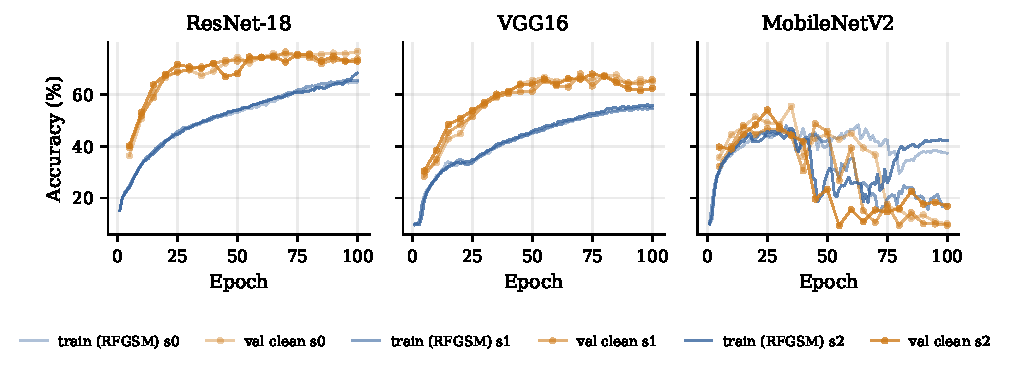
\includegraphics[width=\textwidth]{train_curves}
    \caption[Training curves of the multi-seed adversarially trained models]{Training curves of the multi-seed adversarially trained models: RFGSM training accuracy (blue, every epoch) and clean validation accuracy at $T = 8$ (orange, every five epochs) for seeds 0--2. MobileNetV2 training is unstable, and one seed's training accuracy collapses after about epoch 40.}
    \label{fig:train-curves}
\end{figure}

\begin{table}[htbp]
\centering
\caption[SynOps of fixed-timestep inference]{Mean SynOps per image ($10^6$) of fixed-timestep inference at each horizon (test set).}
\label{tab:app-fixed-synops}
\footnotesize
\begin{tabular}{@{}l rrrrrrrr@{}}
\toprule
Configuration & $T{=}1$ & 2 & 3 & 4 & 5 & 6 & 7 & 8 \\
\midrule
R18 clean & 17.1 & 78.7 & 127.0 & 191.8 & 237.3 & 304.7 & 349.5 & 413.7 \\
R18 adv (1) & 22.1 & 65.2 & 112.0 & 156.9 & 196.1 & 246.9 & 285.7 & 333.3 \\
R18 adv (2) & 10.6 & 56.5 & 89.9 & 138.6 & 164.1 & 218.9 & 240.9 & 292.6 \\
R18 clean mixT & 42.2 & 122.0 & 191.3 & 270.0 & 338.9 & 418.9 & 487.0 & 565.0 \\
R18 adv mixT & 33.2 & 90.9 & 144.4 & 200.7 & 254.2 & 312.2 & 364.4 & 420.4 \\
VGG clean & 4.3 & 28.5 & 51.3 & 81.4 & 100.9 & 132.5 & 151.4 & 182.3 \\
VGG adv & 4.5 & 20.4 & 38.1 & 59.0 & 73.9 & 96.5 & 110.9 & 133.3 \\
MBv2 clean & 45.3 & 92.3 & 139.4 & 187.7 & 234.0 & 282.6 & 328.7 & 377.0 \\
MBv2 adv & 45.9 & 96.2 & 146.4 & 196.9 & 245.4 & 296.7 & 345.0 & 395.8 \\
\bottomrule
\end{tabular}
\end{table}

\begin{table}[htbp]
\centering
\caption{VT sweep for R18 clean (test set, max-softmax rule).}
\label{tab:app-vt-r18_clean_T8}
\footnotesize
\begin{tabular}{@{}c r r r@{}}
\toprule
$\theta$ & Accuracy (\%) & Mean depth & SynOps ($10^6$) \\
\midrule
0.50 & 86.53 & 2.12 & 84.7 \\
0.60 & 87.72 & 2.24 & 90.9 \\
0.70 & 88.91 & 2.39 & 99.4 \\
0.80 & 89.80 & 2.62 & 111.4 \\
0.85 & 90.13 & 2.79 & 120.7 \\
0.90 & 90.62 & 3.01 & 133.0 \\
0.95 & 90.96 & 3.37 & 152.6 \\
0.99 & 91.26 & 4.22 & 199.4 \\
\bottomrule
\end{tabular}
\end{table}

\begin{table}[htbp]
\centering
\caption{VT sweep for R18 adv (1) (test set, max-softmax rule).}
\label{tab:app-vt-r18_adv_T8}
\footnotesize
\begin{tabular}{@{}c r r r@{}}
\toprule
$\theta$ & Accuracy (\%) & Mean depth & SynOps ($10^6$) \\
\midrule
0.50 & 71.48 & 4.33 & 163.3 \\
0.60 & 72.83 & 5.01 & 193.3 \\
0.70 & 73.49 & 5.58 & 219.2 \\
0.80 & 73.66 & 6.11 & 243.4 \\
0.85 & 73.69 & 6.40 & 256.4 \\
0.90 & 73.73 & 6.71 & 271.2 \\
0.95 & 73.73 & 7.10 & 289.2 \\
0.99 & 73.73 & 7.61 & 314.0 \\
\bottomrule
\end{tabular}
\end{table}

\begin{table}[htbp]
\centering
\caption{VT sweep for R18 adv (2) (test set, max-softmax rule).}
\label{tab:app-vt-r18_adv_T8_rep}
\footnotesize
\begin{tabular}{@{}c r r r@{}}
\toprule
$\theta$ & Accuracy (\%) & Mean depth & SynOps ($10^6$) \\
\midrule
0.50 & 75.15 & 4.54 & 151.6 \\
0.60 & 76.42 & 5.13 & 174.7 \\
0.70 & 76.83 & 5.62 & 194.2 \\
0.80 & 77.13 & 6.14 & 215.2 \\
0.85 & 77.16 & 6.41 & 226.0 \\
0.90 & 77.20 & 6.73 & 239.0 \\
0.95 & 77.19 & 7.14 & 255.9 \\
0.99 & 77.19 & 7.69 & 279.0 \\
\bottomrule
\end{tabular}
\end{table}

\begin{table}[htbp]
\centering
\caption{VT sweep for R18 clean mixT (test set, max-softmax rule).}
\label{tab:app-vt-r18_clean_mixT}
\footnotesize
\begin{tabular}{@{}c r r r@{}}
\toprule
$\theta$ & Accuracy (\%) & Mean depth & SynOps ($10^6$) \\
\midrule
0.50 & 52.47 & 1.20 & 58.1 \\
0.60 & 59.63 & 1.38 & 72.0 \\
0.70 & 66.26 & 1.63 & 91.0 \\
0.80 & 72.90 & 1.98 & 117.4 \\
0.85 & 76.39 & 2.23 & 136.1 \\
0.90 & 80.03 & 2.57 & 161.1 \\
0.95 & 84.15 & 3.12 & 201.7 \\
0.99 & 88.92 & 4.24 & 284.8 \\
\bottomrule
\end{tabular}
\end{table}

\begin{table}[htbp]
\centering
\caption{VT sweep for R18 adv mixT (test set, max-softmax rule).}
\label{tab:app-vt-r18_adv_mixT}
\footnotesize
\begin{tabular}{@{}c r r r@{}}
\toprule
$\theta$ & Accuracy (\%) & Mean depth & SynOps ($10^6$) \\
\midrule
0.50 & 70.60 & 3.16 & 146.8 \\
0.60 & 74.70 & 3.98 & 191.1 \\
0.70 & 76.47 & 4.73 & 231.8 \\
0.80 & 77.50 & 5.43 & 270.7 \\
0.85 & 77.63 & 5.78 & 290.3 \\
0.90 & 77.74 & 6.18 & 313.0 \\
0.95 & 77.75 & 6.70 & 342.9 \\
0.99 & 77.75 & 7.42 & 385.1 \\
\bottomrule
\end{tabular}
\end{table}

\begin{table}[htbp]
\centering
\caption{VT sweep for VGG clean (test set, max-softmax rule).}
\label{tab:app-vt-vgg_clean_T8}
\footnotesize
\begin{tabular}{@{}c r r r@{}}
\toprule
$\theta$ & Accuracy (\%) & Mean depth & SynOps ($10^6$) \\
\midrule
0.50 & 84.16 & 2.89 & 49.2 \\
0.60 & 85.78 & 3.20 & 57.1 \\
0.70 & 86.99 & 3.53 & 65.2 \\
0.80 & 87.75 & 3.89 & 74.1 \\
0.85 & 87.94 & 4.08 & 78.9 \\
0.90 & 88.08 & 4.33 & 85.2 \\
0.95 & 88.14 & 4.68 & 94.2 \\
0.99 & 88.18 & 5.46 & 114.3 \\
\bottomrule
\end{tabular}
\end{table}

\begin{table}[htbp]
\centering
\caption{VT sweep for VGG adv (test set, max-softmax rule).}
\label{tab:app-vt-vgg_adv_T8}
\footnotesize
\begin{tabular}{@{}c r r r@{}}
\toprule
$\theta$ & Accuracy (\%) & Mean depth & SynOps ($10^6$) \\
\midrule
0.50 & 64.64 & 5.74 & 86.6 \\
0.60 & 65.21 & 6.27 & 97.0 \\
0.70 & 65.41 & 6.69 & 105.3 \\
0.80 & 65.49 & 7.05 & 112.6 \\
0.85 & 65.48 & 7.21 & 115.9 \\
0.90 & 65.49 & 7.39 & 119.6 \\
0.95 & 65.49 & 7.60 & 124.2 \\
0.99 & 65.49 & 7.87 & 130.2 \\
\bottomrule
\end{tabular}
\end{table}

\begin{table}[htbp]
\centering
\caption{VT sweep for MBv2 clean (test set, max-softmax rule).}
\label{tab:app-vt-mbv2_clean_T8}
\footnotesize
\begin{tabular}{@{}c r r r@{}}
\toprule
$\theta$ & Accuracy (\%) & Mean depth & SynOps ($10^6$) \\
\midrule
0.50 & 28.96 & 2.38 & 110.4 \\
0.60 & 39.32 & 2.95 & 137.6 \\
0.70 & 49.96 & 3.67 & 171.7 \\
0.80 & 60.53 & 4.61 & 216.0 \\
0.85 & 66.50 & 5.17 & 242.9 \\
0.90 & 71.33 & 5.80 & 272.7 \\
0.95 & 75.68 & 6.56 & 308.6 \\
0.99 & 78.08 & 7.41 & 349.2 \\
\bottomrule
\end{tabular}
\end{table}

\begin{table}[htbp]
\centering
\caption{VT sweep for MBv2 adv (test set, max-softmax rule).}
\label{tab:app-vt-mbv2_adv_T8}
\footnotesize
\begin{tabular}{@{}c r r r@{}}
\toprule
$\theta$ & Accuracy (\%) & Mean depth & SynOps ($10^6$) \\
\midrule
0.50 & 49.65 & 6.55 & 323.2 \\
0.60 & 50.92 & 7.21 & 356.2 \\
0.70 & 51.38 & 7.62 & 377.0 \\
0.80 & 51.48 & 7.86 & 388.9 \\
0.85 & 51.49 & 7.93 & 392.3 \\
0.90 & 51.49 & 7.97 & 394.5 \\
0.95 & 51.49 & 8.00 & 395.6 \\
0.99 & 51.49 & 8.00 & 395.8 \\
\bottomrule
\end{tabular}
\end{table}

\begin{table}[htbp]
\centering
\caption[Compute at the VT-neutral operating points]{Compute at the VT-neutral operating points ($\delta = 1$, test set). Mismatch: VT SynOps relative to the matched control. CI: binomial 95\% half-width of the VT accuracy.}
\label{tab:app-neutral-synops}
\footnotesize
\begin{tabular}{@{}l c r c r r r r@{}}
\toprule
Configuration & $\theta$ & VT SynOps & $T^*$ & Matched SynOps & Mismatch & $T{=}8$ SynOps & CI \\
\midrule
R18 clean & 0.90 & 133.0 & 3 & 127.0 & +4.7\% & 413.7 & $\pm$0.57 \\
R18 adv (1) & 0.60 & 193.3 & 5 & 196.1 & -1.5\% & 333.3 & $\pm$0.87 \\
R18 adv (2) & 0.60 & 174.7 & 5 & 164.1 & +6.5\% & 292.6 & $\pm$0.83 \\
R18 clean mixT & 0.99 & 284.8 & 4 & 270.0 & +5.5\% & 565.0 & $\pm$0.62 \\
R18 adv mixT & 0.80 & 270.7 & 5 & 254.2 & +6.5\% & 420.4 & $\pm$0.82 \\
VGG clean & 0.80 & 74.1 & 4 & 81.4 & -8.9\% & 182.3 & $\pm$0.64 \\
VGG adv & 0.50 & 86.6 & 6 & 96.5 & -10.2\% & 133.3 & $\pm$0.94 \\
MBv2 clean & 0.99 & 349.2 & 7 & 328.7 & +6.2\% & 377.0 & $\pm$0.81 \\
MBv2 adv & 0.60 & 356.2 & 7 & 345.0 & +3.2\% & 395.8 & $\pm$0.98 \\
\bottomrule
\end{tabular}
\end{table}

\begin{table}[htbp]
\centering
\caption[Stopping rules at degenerate reference depths]{Stopping-rule results for the two configurations whose reference depth came from a degenerate max-gain operating point (test set).}
\label{tab:app-stoprules-degenerate}
\footnotesize
\begin{tabular}{@{}l l r r@{}}
\toprule
Configuration & Rule & Accuracy (\%) & Mean depth \\
\midrule
R18 clean mixT & fixed T8 baseline & 90.57 & 8.00 \\
R18 clean mixT & max softmax & 59.63 & 1.38 \\
R18 clean mixT & margin & 65.36 & 1.62 \\
R18 clean mixT & entropy & 55.87 & 1.26 \\
R18 clean mixT & temperature softmax & 72.24 & 1.84 \\
R18 clean mixT & evidential surrogate & 45.15 & 1.05 \\
\addlinespace
MBv2 clean & fixed T8 baseline & 77.66 & 8.00 \\
MBv2 clean & max softmax & 28.96 & 2.38 \\
MBv2 clean & margin & 48.82 & 3.58 \\
MBv2 clean & entropy & 29.92 & 2.45 \\
MBv2 clean & temperature softmax & 57.05 & 4.29 \\
MBv2 clean & evidential surrogate & 18.10 & 2.00 \\
\bottomrule
\end{tabular}
\end{table}

{\footnotesize\setlength{\tabcolsep}{3pt}
\begin{longtable}{@{}l l c l l l r r r@{}}
\caption[All single-run attack results]{All single-run attack results, including the neighbouring thresholds of each attacked VT operating point. The run-1 adversarial ResNet-18 is omitted (see \secref{sec:res-threats}).}\label{tab:app-attacks}\\
\toprule
Configuration & Mode & $\theta$ & Role & Attack & Objective & Acc. & Depth & $n$ \\
\midrule
\endfirsthead
\toprule
Configuration & Mode & $\theta$ & Role & Attack & Objective & Acc. & Depth & $n$ \\
\midrule
\endhead
R18 clean & fixed & --- & fixed T8 baseline & pgd & untargeted & 0.00 & 8.00 & 10000 \\
R18 clean & vt & 0.60 & lower neighbor & pgd & untargeted & 0.00 & 2.00 & 10000 \\
R18 clean & vt & 0.70 & selected & pgd & untargeted & 0.02 & 2.00 & 10000 \\
R18 clean & vt & 0.80 & upper neighbor & pgd & untargeted & 0.00 & 2.01 & 10000 \\
R18 clean & vt & 0.60 & lower neighbor & pgd & wrong early exit & 0.00 & 2.00 & 10000 \\
R18 clean & vt & 0.70 & selected & pgd & wrong early exit & 0.00 & 2.00 & 10000 \\
R18 clean & vt & 0.80 & upper neighbor & pgd & wrong early exit & 0.00 & 2.00 & 10000 \\
R18 clean & vt & 0.60 & lower neighbor & pgd & compute overuse & 59.74 & 3.09 & 10000 \\
R18 clean & vt & 0.70 & selected & pgd & compute overuse & 60.58 & 3.58 & 10000 \\
R18 clean & vt & 0.80 & upper neighbor & pgd & compute overuse & 63.10 & 4.23 & 10000 \\
R18 clean & fixed & --- & fixed T8 baseline & autoattack & untargeted & 0.06 & 8.00 & 10000 \\
R18 clean & vt & 0.70 & selected & autoattack & untargeted & 0.02 & 2.14 & 10000 \\
\addlinespace
R18 adv (2) & fixed & --- & fixed T8 baseline & pgd & untargeted & 46.10 & 8.00 & 2000 \\
R18 adv (2) & vt & 0.50 & lower neighbor & pgd & untargeted & 47.75 & 5.13 & 2000 \\
R18 adv (2) & vt & 0.60 & selected & pgd & untargeted & 48.70 & 5.86 & 2000 \\
R18 adv (2) & vt & 0.70 & upper neighbor & pgd & untargeted & 46.35 & 6.43 & 2000 \\
R18 adv (2) & vt & 0.50 & lower neighbor & pgd & wrong early exit & 45.80 & 4.75 & 2000 \\
R18 adv (2) & vt & 0.60 & selected & pgd & wrong early exit & 45.95 & 5.62 & 2000 \\
R18 adv (2) & vt & 0.70 & upper neighbor & pgd & wrong early exit & 47.75 & 6.31 & 2000 \\
R18 adv (2) & vt & 0.50 & lower neighbor & pgd & compute overuse & 88.90 & 4.84 & 2000 \\
R18 adv (2) & vt & 0.60 & selected & pgd & compute overuse & 92.00 & 5.40 & 2000 \\
R18 adv (2) & vt & 0.70 & upper neighbor & pgd & compute overuse & 93.25 & 6.04 & 2000 \\
R18 adv (2) & fixed & --- & fixed T8 baseline & autoattack & untargeted & 28.85 & 8.00 & 2000 \\
R18 adv (2) & vt & 0.60 & selected & autoattack & untargeted & 24.15 & 5.55 & 2000 \\
\addlinespace
R18 clean mixT & fixed & --- & fixed T8 baseline & pgd & untargeted & 0.00 & 8.00 & 2000 \\
R18 clean mixT & vt & 0.50 & lower neighbor & pgd & untargeted & 0.15 & 1.01 & 2000 \\
R18 clean mixT & vt & 0.60 & selected & pgd & untargeted & 0.15 & 1.02 & 2000 \\
R18 clean mixT & vt & 0.70 & upper neighbor & pgd & untargeted & 0.10 & 1.05 & 2000 \\
R18 clean mixT & vt & 0.50 & lower neighbor & pgd & wrong early exit & 3.35 & 1.10 & 2000 \\
R18 clean mixT & vt & 0.60 & selected & pgd & wrong early exit & 2.60 & 1.18 & 2000 \\
R18 clean mixT & vt & 0.70 & upper neighbor & pgd & wrong early exit & 2.10 & 1.25 & 2000 \\
R18 clean mixT & vt & 0.50 & lower neighbor & pgd & compute overuse & 85.40 & 1.21 & 2000 \\
R18 clean mixT & vt & 0.60 & selected & pgd & compute overuse & 81.60 & 1.55 & 2000 \\
R18 clean mixT & vt & 0.70 & upper neighbor & pgd & compute overuse & 75.30 & 2.08 & 2000 \\
R18 clean mixT & fixed & --- & fixed T8 baseline & autoattack & untargeted & 0.10 & 8.00 & 2000 \\
R18 clean mixT & vt & 0.60 & selected & autoattack & untargeted & 2.25 & 1.13 & 2000 \\
\addlinespace
R18 adv mixT & fixed & --- & fixed T8 baseline & pgd & untargeted & 40.85 & 8.00 & 2000 \\
R18 adv mixT & vt & 0.70 & lower neighbor & pgd & untargeted & 40.90 & 5.59 & 2000 \\
R18 adv mixT & vt & 0.80 & selected & pgd & untargeted & 41.50 & 6.35 & 2000 \\
R18 adv mixT & vt & 0.85 & upper neighbor & pgd & untargeted & 40.80 & 6.77 & 2000 \\
R18 adv mixT & vt & 0.70 & lower neighbor & pgd & wrong early exit & 42.00 & 5.35 & 2000 \\
R18 adv mixT & vt & 0.80 & selected & pgd & wrong early exit & 42.55 & 6.27 & 2000 \\
R18 adv mixT & vt & 0.85 & upper neighbor & pgd & wrong early exit & 41.80 & 6.66 & 2000 \\
R18 adv mixT & vt & 0.70 & lower neighbor & pgd & compute overuse & 93.80 & 5.30 & 2000 \\
R18 adv mixT & vt & 0.80 & selected & pgd & compute overuse & 94.95 & 6.08 & 2000 \\
R18 adv mixT & vt & 0.85 & upper neighbor & pgd & compute overuse & 95.70 & 6.54 & 2000 \\
R18 adv mixT & fixed & --- & fixed T8 baseline & autoattack & untargeted & 29.45 & 8.00 & 2000 \\
R18 adv mixT & vt & 0.80 & selected & autoattack & untargeted & 25.55 & 5.98 & 2000 \\
\addlinespace
VGG clean & fixed & --- & fixed T8 baseline & pgd & untargeted & 0.05 & 8.00 & 2000 \\
VGG clean & vt & 0.60 & lower neighbor & pgd & untargeted & 0.10 & 2.32 & 2000 \\
VGG clean & vt & 0.70 & selected & pgd & untargeted & 0.10 & 2.40 & 2000 \\
VGG clean & vt & 0.80 & upper neighbor & pgd & untargeted & 0.05 & 2.52 & 2000 \\
VGG clean & vt & 0.60 & lower neighbor & pgd & wrong early exit & 0.10 & 2.32 & 2000 \\
VGG clean & vt & 0.70 & selected & pgd & wrong early exit & 0.00 & 2.45 & 2000 \\
VGG clean & vt & 0.80 & upper neighbor & pgd & wrong early exit & 0.10 & 2.62 & 2000 \\
VGG clean & vt & 0.60 & lower neighbor & pgd & compute overuse & 69.80 & 3.99 & 2000 \\
VGG clean & vt & 0.70 & selected & pgd & compute overuse & 72.10 & 4.70 & 2000 \\
VGG clean & vt & 0.80 & upper neighbor & pgd & compute overuse & 75.40 & 5.41 & 2000 \\
VGG clean & fixed & --- & fixed T8 baseline & autoattack & untargeted & 0.00 & 8.00 & 2000 \\
VGG clean & vt & 0.70 & selected & autoattack & untargeted & 0.00 & 2.82 & 2000 \\
\addlinespace
VGG adv & fixed & --- & fixed T8 baseline & pgd & untargeted & 45.90 & 8.00 & 2000 \\
VGG adv & vt & 0.50 & lower neighbor & pgd & untargeted & 44.95 & 6.17 & 2000 \\
VGG adv & vt & 0.60 & selected & pgd & untargeted & 44.45 & 6.69 & 2000 \\
VGG adv & vt & 0.70 & upper neighbor & pgd & untargeted & 44.75 & 7.13 & 2000 \\
VGG adv & vt & 0.50 & lower neighbor & pgd & wrong early exit & 45.40 & 5.98 & 2000 \\
VGG adv & vt & 0.60 & selected & pgd & wrong early exit & 46.35 & 6.62 & 2000 \\
VGG adv & vt & 0.70 & upper neighbor & pgd & wrong early exit & 46.70 & 7.05 & 2000 \\
VGG adv & vt & 0.50 & lower neighbor & pgd & compute overuse & 79.25 & 5.83 & 2000 \\
VGG adv & vt & 0.60 & selected & pgd & compute overuse & 80.95 & 6.31 & 2000 \\
VGG adv & vt & 0.70 & upper neighbor & pgd & compute overuse & 81.45 & 6.80 & 2000 \\
VGG adv & fixed & --- & fixed T8 baseline & autoattack & untargeted & 10.75 & 8.00 & 2000 \\
VGG adv & vt & 0.60 & selected & autoattack & untargeted & 8.55 & 6.60 & 2000 \\
\addlinespace
MBv2 clean & fixed & --- & fixed T8 baseline & pgd & untargeted & 5.10 & 8.00 & 2000 \\
MBv2 clean & vt & 0.90 & lower neighbor & pgd & untargeted & 4.30 & 6.55 & 2000 \\
MBv2 clean & vt & 0.95 & selected & pgd & untargeted & 4.95 & 7.17 & 2000 \\
MBv2 clean & vt & 0.99 & upper neighbor & pgd & untargeted & 4.85 & 7.86 & 2000 \\
MBv2 clean & vt & 0.90 & lower neighbor & pgd & wrong early exit & 4.20 & 6.22 & 2000 \\
MBv2 clean & vt & 0.95 & selected & pgd & wrong early exit & 4.05 & 6.95 & 2000 \\
MBv2 clean & vt & 0.99 & upper neighbor & pgd & wrong early exit & 3.80 & 7.82 & 2000 \\
MBv2 clean & vt & 0.90 & lower neighbor & pgd & compute overuse & 97.05 & 7.38 & 2000 \\
MBv2 clean & vt & 0.95 & selected & pgd & compute overuse & 97.20 & 7.71 & 2000 \\
MBv2 clean & vt & 0.99 & upper neighbor & pgd & compute overuse & 97.10 & 7.99 & 2000 \\
MBv2 clean & fixed & --- & fixed T8 baseline & autoattack & untargeted & 5.25 & 8.00 & 2000 \\
MBv2 clean & vt & 0.95 & selected & autoattack & untargeted & 5.40 & 7.23 & 2000 \\
\addlinespace
MBv2 adv & fixed & --- & fixed T8 baseline & pgd & untargeted & 35.60 & 8.00 & 2000 \\
MBv2 adv & vt & 0.50 & lower neighbor & pgd & untargeted & 34.55 & 6.85 & 2000 \\
MBv2 adv & vt & 0.60 & selected & pgd & untargeted & 34.75 & 7.45 & 2000 \\
MBv2 adv & vt & 0.70 & upper neighbor & pgd & untargeted & 35.80 & 7.79 & 2000 \\
MBv2 adv & vt & 0.50 & lower neighbor & pgd & wrong early exit & 34.50 & 6.69 & 2000 \\
MBv2 adv & vt & 0.60 & selected & pgd & wrong early exit & 33.35 & 7.42 & 2000 \\
MBv2 adv & vt & 0.70 & upper neighbor & pgd & wrong early exit & 32.90 & 7.78 & 2000 \\
MBv2 adv & vt & 0.50 & lower neighbor & pgd & compute overuse & 64.40 & 6.59 & 2000 \\
MBv2 adv & vt & 0.60 & selected & pgd & compute overuse & 67.10 & 7.26 & 2000 \\
MBv2 adv & vt & 0.70 & upper neighbor & pgd & compute overuse & 66.70 & 7.68 & 2000 \\
MBv2 adv & fixed & --- & fixed T8 baseline & autoattack & untargeted & 27.60 & 8.00 & 2000 \\
MBv2 adv & vt & 0.60 & selected & autoattack & untargeted & 27.55 & 7.39 & 2000 \\
\bottomrule
\end{longtable}}

\begin{table}[htbp]
\centering
\caption[Attack-seed variance]{Attack-seed variance: robust accuracy (\%, mean $\pm$ SD over three attack seeds) on one adversarially trained checkpoint per backbone ($n = 1{,}000$).}
\label{tab:app-attack-seed}
\footnotesize
\begin{tabular}{@{}l rr rr rr@{}}
\toprule
& \multicolumn{2}{c}{Full $T{=}8$} & \multicolumn{2}{c}{Matched} & \multicolumn{2}{c}{VT} \\
\cmidrule(lr){2-3} \cmidrule(lr){4-5} \cmidrule(l){6-7}
Backbone & PGD & AA & PGD & AA & PGD & AA \\
\midrule
ResNet-18 & 56.8 $\pm$ 0.70 & 32.0 $\pm$ 0.31 & 55.1 $\pm$ 1.14 & 23.9 $\pm$ 0.44 & 56.3 $\pm$ 1.33 & 23.2 $\pm$ 1.74 \\
VGG16 & 45.0 $\pm$ 1.00 & 18.4 $\pm$ 0.12 & 43.8 $\pm$ 0.26 & 20.4 $\pm$ 0.45 & 45.2 $\pm$ 0.55 & 16.0 $\pm$ 0.81 \\
MobileNetV2 & 45.5 $\pm$ 0.78 & 20.6 $\pm$ 0.46 & 41.2 $\pm$ 1.04 & 13.4 $\pm$ 0.66 & 44.4 $\pm$ 0.85 & 10.8 $\pm$ 0.40 \\
\bottomrule
\end{tabular}
\end{table}

\begin{table}[htbp]
\centering
\caption[Multi-seed training summaries]{Multi-seed training summaries (adversarial fixed-T8 regime). Train adv.: RFGSM training accuracy in the final epoch. Best val.: best clean validation accuracy at $T = 8$ (evaluated every five epochs).}
\label{tab:app-train}
\footnotesize
\begin{tabular}{@{}l c c r r@{}}
\toprule
Backbone & Seed & Epochs & Train adv.\ (\%) & Best val.\ (\%) \\
\midrule
ResNet-18 & 0 & 100 & 64.81 & 76.56 \\
ResNet-18 & 1 & 100 & 65.47 & 76.38 \\
ResNet-18 & 2 & 100 & 68.25 & 75.48 \\
VGG16 & 0 & 100 & 55.00 & 67.52 \\
VGG16 & 1 & 100 & 54.42 & 67.90 \\
VGG16 & 2 & 100 & 55.72 & 67.86 \\
MobileNetV2 & 0 & 100 & 37.26 & 55.46 \\
MobileNetV2 & 1 & 100 & 17.49 & 48.66 \\
MobileNetV2 & 2 & 100 & 42.11 & 54.02 \\
\bottomrule
\end{tabular}
\end{table}


\chapter{Reproducibility}
\label{app:repro}

\section{Repository Layout}

The experimental code and all raw results are kept in a single repository.

\begin{itemize}
    \item \texttt{model.py}, \texttt{stopping.py}, \texttt{metrics.py}, \texttt{attacks.py}, \texttt{training.py}, \texttt{experiments.py}, \texttt{data.py}, \texttt{configs.py}: the experimental suite (models and LIF neurons, stopping rules, SynOps monitor, attacks, training loop, evaluation protocol, data splits, configuration dataclasses).
    \item \texttt{build\_vanilla\_\{resnet18,vgg16,mobilenetv2\}\_kaggle\_notebook.py}: builders for the self-contained single-run notebooks. The ResNet-18 builder emits four notebooks, one for each regime--schedule combination.
    \item \texttt{build\_multiseed\_kaggle\_notebook.py}: builder for the multi-seed notebooks (one per backbone), including training of every seed.
    \item \texttt{Findings/}: one folder of raw CSV results per configuration (calibration and test sweeps, matched controls, selected thresholds, stopping rules, attack results) and per multi-seed run (per-checkpoint results, attack-seed results, training histories).
    \item \texttt{thesis report/vt\_thesis/analysis/}: \texttt{build\_facts.py} (computes every number in the thesis and writes \texttt{facts.json} and \texttt{facts.md}), \texttt{make\_figures.py} (all data figures and the pooled statistics) and \texttt{make\_tables.py} (appendix tables).
\end{itemize}

\section{Regenerating the Results}

\paragraph{Training and evaluation.} Each notebook is generated by running its builder script locally and uploaded to Kaggle with a GPU accelerator. With internet disabled, CIFAR-10 and the AutoAttack and torchattacks packages must be attached as Kaggle datasets, and the notebooks locate them automatically. Training regime and schedule are selected by the \texttt{TRAIN\_REGIME} and \texttt{TRAIN\_SCHEDULE} variables at the top of the configuration cell. Each notebook writes its CSV results and checkpoint to the Kaggle working directory.

\paragraph{Analysis.} With the results unpacked into \texttt{Findings/}, the analysis is regenerated from the thesis directory with
\begin{lstlisting}[basicstyle=\ttfamily\small, columns=fullflexible]
python analysis/build_facts.py
python analysis/make_figures.py
python analysis/make_tables.py
\end{lstlisting}
No GPU is needed for the analysis: operating-point re-selection, compute matching and all statistics are computed from the saved sweeps.

\paragraph{Document.} The thesis is compiled with Tectonic (XeTeX engine) and Biber:
\begin{lstlisting}[basicstyle=\ttfamily\small, columns=fullflexible]
tectonic -X compile main.tex
\end{lstlisting}
The Biber version must match the biblatex version bundled with Tectonic (Biber 2.17 for Tectonic 0.17).

\section{Determinism}

All models use deterministic neurons, and data splits, attack subsets and training seeds are fixed. Results may still differ in the last digit between runs because of non-deterministic cuDNN kernels, TF32 arithmetic and mixed precision. The multi-seed experiments quantify run-to-run variance at the level that matters for our conclusions.

\end{appendices}

\end{document}
